% SPDX-License-Identifier: CC-BY-4.0
% =====================================================================
% D. Joyner and Claude, "On the transfer of Shalika germs for G_2"
% Draft 1. Corrected and expanded version, November 2026.
%
% Built from ../transcription/g2_shalika_germs_transcription.tex (the literal
% transcription of the 1994 manuscript in ../original-1994/) and the referee
% report ../referee/g2_referee_report.tex. Every change from the 1994 text is
% either clear-cut (recorded in CHANGES.md) or flagged in the text by a
% "Remark 2026.n". Comments beginning "% [Claude]" are editorial notes.
% Numbering of sections, equations and results follows the 1994 manuscript;
% items added in 2026 carry letters (Proposition 3.4A, Table 4.3A).
% History of the drafts: ../revision_log.md.
% =====================================================================
\documentclass[12pt,letterpaper]{amsart}
\usepackage[T1]{fontenc}
% Times for text and math. The style guide prefers newtx; it was not
% installed where this draft was built, so the fallback mathptmx is used.
% To switch, replace the next line by \usepackage{newtxtext,newtxmath}.
\usepackage{mathptmx}
\usepackage{courier}
\usepackage[letterpaper,margin=1in]{geometry}
\usepackage{amsmath,amssymb,amsthm,amscd}
\usepackage{enumitem,booktabs,longtable,xparse}
\usepackage{tikz}
\usepackage{microtype}
\usepackage[hidelinks]{hyperref}
\setlist{itemsep=2pt,topsep=4pt}
\setlength{\emergencystretch}{3em}
\allowdisplaybreaks

% ---------- numbering ----------
% Results and equations keep the numbers of the 1994 manuscript. A result is
% written \begin{res}{Lemma}{3.5}[optional title] ... \end{res}; it prints
% "Lemma 3.5" and makes "3.5" available to \label and \ref. Equations use
% \tag{n}\label{eq:n}. Remarks 2026.n are numbered automatically.
\makeatletter
\newcommand{\res@name}{}
\theoremstyle{plain}
\newtheorem*{resplain@}{\res@name}
\NewDocumentEnvironment{res}{m m o}
  {\def\res@name{#1 #2}\phantomsection\def\@currentlabel{#2}%
   \IfNoValueTF{#3}{\begin{resplain@}}{\begin{resplain@}[{#3}]}}{\end{resplain@}}
\theoremstyle{definition}
\newtheorem*{resdef@}{\res@name}
\NewDocumentEnvironment{resdef}{m m o}
  {\def\res@name{#1 #2}\phantomsection\def\@currentlabel{#2}%
   \IfNoValueTF{#3}{\begin{resdef@}}{\begin{resdef@}[{#3}]}}{\end{resdef@}}
% \fixedlabel{3.2a}: give the next \label a fixed number.
\newcommand{\fixedlabel}[1]{\phantomsection\def\@currentlabel{#1}}
% \numsection{1}{Title}: a section heading carrying the 1994 number.
\newcommand{\numsection}[2]{\section*{\S\,#1\quad #2}\phantomsection
  \def\@currentlabel{#1}}
\makeatother
% Remarks 2026.n: caveats, gaps, and statements not fully verified.
\newcounter{rtw}
\renewcommand{\thertw}{2026.\arabic{rtw}}
\newcommand{\jremname}{}
\theoremstyle{remark}
\newtheorem*{genrem}{\jremname}
\NewDocumentEnvironment{rem26}{o}
  {\refstepcounter{rtw}\renewcommand\jremname{Remark \thertw}%
   \IfNoValueTF{#1}{\begin{genrem}}{\begin{genrem}[{#1}]}}{\end{genrem}}
\theoremstyle{definition}
\newtheorem*{example}{Example}

% ---------- notation ----------
\newcommand{\ovF}{\overline{F}}
\newcommand{\OF}{\mathcal{O}_F}
\newcommand{\ooo}{\mathcal{O}}
\newcommand{\ovo}{\overline{\mathcal{O}}}
\newcommand{\aaa}{\mathbb{A}}
\newcommand{\zzz}{\mathbb{Z}}
\newcommand{\rrr}{\mathbb{R}}
\newcommand{\qqq}{\mathbb{Q}}
\newcommand{\gga}{\mathbb{G}}
\newcommand{\eps}{\epsilon}
\newcommand{\unx}{\underline{x}}
\newcommand{\iddots}{\mathinner{\mkern1mu\raise1pt\hbox{.}\mkern2mu%
  \raise4pt\hbox{.}\mkern2mu\raise7pt\vbox{\kern7pt\hbox{.}}\mkern1mu}}
\DeclareMathOperator{\Ind}{Ind}
\DeclareMathOperator{\Cent}{Cent}
\DeclareMathOperator{\Gal}{Gal}
\DeclareMathOperator{\inv}{inv}
\DeclareMathOperator{\supp}{supp}
\DeclareMathOperator{\Lie}{Lie}
\DeclareMathOperator{\Ad}{Ad}
\DeclareMathOperator{\diag}{diag}

\title[Transfer of Shalika germs for $G_2$]{On the transfer of Shalika germs for $G_2$\\[4pt]
\normalsize Draft 1. Corrected and expanded version}
\author{David Joyner}
\thanks{This is a revision of the unpublished manuscript of the same title by
D.~Joyner, dated summer 1994. The 1994 AMS-TeX source, a literal transcription
and a referee report are in the directory \texttt{g2stuff} of the repository
\texttt{github.com/wdjoyner/trace-formulas}. The revision was made in November
2026. Gaps, caveats and statements not fully verified are collected in the
numbered ``Remarks 2026.$n$''.}
\email{wdjoyner@gmail.com}
\author{Claude}
\thanks{Claude is an AI model made by Anthropic. See the Acknowledgments for
the division of work.}
\date{Original draft: 1994. Corrected and expanded draft: 2026}

\begin{document}

\begin{abstract}
This revision was prepared with the help of an AI system: Claude (Anthropic)
refereed the 1994 manuscript and drafted this revision as a co-author. See the
Acknowledgments for details. Let $G_2$ be the split exceptional group over a
$p$-adic field $F$. Using Langlands' method, based on Igusa's asymptotic
expansions, we study the $\kappa$-Shalika germs of $G_2$ attached to the
$1$-, $2$- and $3$-regular unipotent classes. We construct the variety $Z$
underlying Langlands' partial resolution, prove that $Z$ is normal and
Cohen--Macaulay, cover it up to codimension two by explicit regular patches,
and compute the Igusa constants of every branch of the special fiber. The
$2$- and $3$-regular classes are carried by unique base divisors, with Igusa
constants $3$ and $4$, matching the trivial classes of the cuspidal
endoscopic groups $(SL(2)\times SL(2))/\{\pm1\}$ and $PGL(3)$. We list all
elliptic endoscopic data of $G_2$. The 1994 manuscript claimed to deduce the
matching of these germs, and hence local transfer for $G_2$, from a reduction
lemma of Hales. That lemma does not apply to $G_2$, so the matching theorems
are stated here as conditional on an explicit computation that remains to be
done (Remark~\ref{rem:main-gap}). The matching itself is now known by other
means, from Waldspurger's transfer theorem and the fundamental lemma.
\end{abstract}

\maketitle
\setcounter{tocdepth}{1}
\tableofcontents
% =====================================================================
% Section 0. Source: g2new0.tex. [Claude] Corrections are listed in CHANGES.md.
% =====================================================================
\numsection{0}{Introduction}\label{sec:0}

This section explains the problem, sketches Langlands' method, states what
the 1994 manuscript set out to prove, and records what this revision proves,
what it proves only conditionally, and what is now known by other means.
The notation is collected in the section ``Notation'' after the literature
review.

\subsection*{Motivation and rough outline}

To apply the trace formula to the transfer of automorphic representations
of two reductive groups $G$, $H$ over a number field $K$, one must,
among other things, have a comparison of local orbital integrals, for each
local completion $F$ of $K$. The comparison in the real and complex case
was solved by Shelstad \cite{She82}.
In the $p$-adic case, such a local comparison (the smooth matching conjecture
stated below) reduces, thanks to the work of R. Langlands and D. Shelstad
(\cite{LS87}, \cite{LS90}), to a certain matching of Shalika germs,
also stated below.
Shalika germs are functions
associated to a semisimple element $s\in G(F)$ and a unipotent
conjugacy class ${\mathcal O}$ of $M=\Cent_{G(F)}(s)$, defined in a punctured
compact-open neighborhood of $s$ in the regular set \cite{Sh72}. They play a
role in the analysis of $p$-adic orbital integrals on reductive groups
roughly analogous to the role that the power functions play in the Taylor
series of a function on the real line. By a well-known reduction known
as Harish-Chandra descent, it usually suffices to assume that $s$ is central
and $M=G$.

Langlands \cite{La83} introduced a geometric approach to the computation,
or at least comparison, of Shalika germs.
The comparison of Shalika germs associated to the
$0$-regular (regular) unipotent classes was solved by Shelstad \cite{She89},
using results from \cite{LS87}, \cite{LS90}.
Langlands's technique was further developed by
T. Hales in his thesis \cite{Ha92a}. Hales concentrated on the comparison of
$1$-regular germs, matching the stable subregular germs in general and
matching the $\kappa$-stable subregular germs for even rank unitary
groups. This technique of Langlands goes by
the name Igusa theory, since it was Igusa \cite{Ig78} who developed a crucial
asymptotic formula for an integral over fibers of a morphism
$Y_C\rightarrow C$, where $C$ is a curve and $Y_C$ is a non-singular
variety. The technique also relies on a formula for the coefficients
of this expansion, involving principal value integrals over $p$-adic
analytic manifolds, worked out in \cite{Ig78}, \cite{La83} (see also
\cite{LS83}). In \cite{La83}, \cite{LS89}, Langlands and Shelstad
matched all the germs for groups of absolute type $A_2$
(see also \cite{Ha92b}, where a descent argument is used instead of
the direct comparison in \cite{LS89}).
In \cite{Ha89}, Hales worked out the comparison of germs for the forms of
$B_2=C_2$ using Igusa theory, a reduction argument, and an explicit
computation of the dependence of the germs on the tangent direction.

The 1994 manuscript set out to verify the matching of Shalika germs
for the $1$-, $2$- and $3$-regular germs of the
exceptional group $G_2$ and to deduce, together with \cite{She89}, the
smooth matching theorem for $G_2$ in the following form.

\begin{res}{Conjecture}{0.0}[Smooth matching for $G_2$]\label{res:smooth}
Let $T_G$ denote an elliptic Cartan subgroup of $G=G_2$ and let $\kappa$
denote a character of $H^1(\Gal(\ovF/F),T_G)$ whose endoscopic group
$H=H(T_G,\kappa)$ is cuspidal (so $H$ is $PGL(3)$ or
$(SL(2)\times SL(2))/\{\pm 1\}$, by Appendix~\ref{sec:A}).
Let $T_H$ denote the image of an admissible embedding of $T_G$ into $H$.
For each $f\in C_c^\infty(G(F))$ there is an $f^H\in C_c^\infty(H(F))$,
depending only on $f$ and $H$, for which
\[
\Delta_{G/H}^{T_G,\kappa}(\gamma_H,\gamma_G)
\Phi^{T_G,\kappa}(\gamma_G,f)
=\Phi^{T_H,st}(\gamma_H,f^H),
\]
whenever $\gamma_G$ is the image of a regular $\gamma_H\in T_H(F)$.
\end{res}

\begin{rem26}[status of Conjecture~\ref{res:smooth}]\label{rem:transfer-known}
The 1994 manuscript called this the smooth matching conjecture and claimed to
prove it. That proof is incomplete (Remark~\ref{rem:main-gap}). The statement
is nevertheless now a theorem: Waldspurger proved that the fundamental lemma
implies transfer \cite{Wa97}, and Ng\^o proved the fundamental lemma
\cite{Ng10}. Gordon and Hales \cite{GH16} derive from Waldspurger's transfer
the matching of all $\kappa$-Shalika germs. (Level 3 for \cite{Wa97},
\cite{Ng10}; level 2 for \cite{GH16}, checked against its abstract and
introduction.) The interest of the Igusa-theoretic approach is therefore not
the existence of transfer, but the explicit geometric description of the
germs and of the matching constants.
\end{rem26}

\medskip
In \S\ref{sec:1} we recall
in detail the construction of the Igusa variety and the
determination of local coordinates \cite{La83}, \cite{Ha92a}, \cite{Ha89}.
Section~\ref{sec:2} gives the calculations for determining the action of the
Galois group on the local coordinates on the
Igusa variety for $G_2$, as in \cite{Ha89}.

Section~\ref{sec:3} introduces, for any reductive group $G$,
specific patches generalizing those used in \cite{Ha89}.
For $G_2$ we show that they are regular and cover the monomial variety $Z$
underlying the base Igusa variety $Y''$ up to codimension two
(Proposition~\ref{res:3.4A}). We also show that, for $G_2$, $Z$ is normal and
Cohen--Macaulay (Proposition~\ref{res:3.7}). This proves Hales'
conjecture \cite{Ha92a} that $Y''$ is regular in codimension one, for $G_2$.

In Section~\ref{sec:4} we compute the Igusa constants of all
the branches of the special fiber of $Z$ (Table~\ref{tab:4.3A})
and give an ``endoscopic interpretation'' of some of them.

In Section~\ref{sec:5} we first record some basic facts about
the Igusa expansion over $Y_C$. We then discuss the
``no spurious divisors lemma'' for $G_2$, which is basically an inequality
$e(\theta,\beta)\leq 1$, where $e(\theta,\beta)$ is as in \cite{La83}.
Its proof is incomplete (Remark~\ref{rem:5.14}). Finally, we recall the
statement of Hales' reduction lemma and explain why it does not apply to the
cuspidal endoscopic groups of $G_2$ (Remark~\ref{rem:main-gap}).

In Sections~\ref{sec:6}, \ref{sec:7} and~\ref{sec:8}
we (a) compute coordinates
on the $1$-, $2$- and $3$-regular unipotent orbits (the latter two
are not Richardson; they are what we call
``endoscopically Richardson''), (b) compute
coordinates on the fiber $\phi^{-1}(\gamma_\lambda)^\Gamma$
(explained below), and (c) express the contribution of each orbit to the
Igusa expansion as a principal value integral over a single base divisor.
One new idea is that, roughly speaking, the subgroup generated by the
one-parameter root-groups associated to roots outside a pseudo-Levi
subgroup $M$ of $G_2$ may be used to determine local coordinates for the
``endoscopically Richardson'' orbit $\ooo=\Ind_M^G(1)$.
The matching theorems of these sections are stated conditionally on an
explicit computation of the dependence of these integrals on the tangent
direction $X$ (Hypotheses $(\mathrm X_r)$ of Remark~\ref{rem:main-gap}).

Section~\ref{sec:9} presents a conjecture which the method seems to support.
The appendix collects explicit group-theoretic computations: a Chevalley basis
of ${\mathfrak g}_2$ via triality, the cuspidal endoscopic groups of $G_2$,
all elliptic endoscopic data (Table~\ref{tab:A.6}), and the stability of
the $2$- and $3$-regular classes.

\subsection*{Langlands' idea}

Here is a rough sketch of Langlands' idea in its simplest form.
Let $\gamma\in G(F)$ be an elliptic regular element and let
$T_G=\Cent_G(\gamma)^o$. The goal is to compute,
or at least find some manageable expression for, the stable orbital
integral $\int_{(T_G\setminus G)(F)}f(g\gamma g^{-1})dg$.
(More generally, one can and does consider $\kappa$-orbital
integrals.) The variety $T_G\setminus G$
may be identified, over the algebraic closure
$\overline{F}$, with the variety of regular stars. Let
$\Omega$ denote the absolute Weyl group of $T_G$,
$B_G$ a Borel subgroup of $G$
containing $T_G$, and $S_0$ the $G(\ovF)$-orbit of the
$|\Omega|$-tuple $(B_G^\omega)_{\omega\in \Omega}$, where
$G$ acts by conjugation on each coordinate. This orbit is called the
variety of regular stars, and since
$\cap_{\omega\in \Omega}N_G(B_G^\omega)=T_G$,
we have $S_0\cong T_G\setminus G$ over $\ovF$. Let
${\mathcal B}\cong B_G\setminus G$
denote the Borel variety. Although ${\mathcal B}$ is complete,
$S_0$ is not. Conjugation induces a principal $N_G$-bundle structure on
$S_0\rightarrow {\mathcal B}$, where $N_G$ denotes
the unipotent radical of $B_G$.
The Zariski closure of
$S_0$ in ${\mathcal B}^{|\Omega|}$ is denoted $S$ and is called the variety of
stars. It is projective but singular, and $S_0$ is Zariski open in $S$.
Roughly speaking, the idea is to regard the above stable orbital integral
as an integral over $S_0(F)\subset S(\ovF)$. Let $T_G'$
denote the subvariety of regular elements of $T_G$. We
restrict $\gamma$ to a curve $C$ in $T'_G\cup \{1\}$
through the identity, and construct a smooth variety $Y_C$
with a fibering $\phi:Y_C\rightarrow C$, ``the''
smooth Igusa variety, whose fibers
$\phi^{-1}(\gamma)$, $\gamma\in C,\ \gamma\not= 1$,
are isomorphic to $T_G\setminus G$. The stable orbital integral
may then be regarded as a fiber integral parameterized by a
local coordinate $\lambda$ in a neighborhood of $1\in C$.
Taking the limit as $\lambda$ tends to $0$,
one may use techniques of Igusa \cite{Ig78}, as developed
by Langlands \cite{La83}, to express the stable orbital integral
as a sum involving principal value integrals over certain divisors
contained in $\phi^{-1}(1) \subset Y_C$. By the homogeneity
of the Shalika germs and of the coefficients in the Igusa expansion, only
certain divisors can contribute to a given Shalika germ.

Here is a rough sketch of Igusa theory \cite{La83}, \cite{Ha92a}.
Assume $G$ is $F$-quasisplit. Let $C$ denote a $1$-parameter subgroup of $G$
in $T_G$, defined over $F$, containing the identity
and no other singular point, and whose tangent over $\ovF$ is not
contained in any root hyperplane. Let $C'=C-\{1\}$. We sketch the
construction of a non-singular algebraic variety $Y_C$, defined over $F$,
for which
\[
\begin{CD}
C'\times T_G\setminus G @> i >> Y_C @> \pi >> G\\
@. @VV \phi V @. \\
@. C, @.
\end{CD}
\]
with the following properties.
\begin{enumerate}[label=(\alph*)]
\item If $T_G$ and $C$ are defined over $F$ then so are
$Y_C$, $\phi$, $\pi$, and $i$.
\item $\pi : Y_C\rightarrow G$ is proper and $G$-equivariant.
\item $\phi : Y_C\rightarrow C$ is proper.
\item $\pi(\phi^{-1}(1))=V$, the unipotent variety of $G$.
\item If ${\mathcal O}\subset G$ is a unipotent orbit and $E\subset
\phi^{-1}(1)$ is a divisor with $\pi(E)=\ovo$, then
$\pi|_{E}:E\cap \pi^{-1}({\mathcal O})\rightarrow {\mathcal O}$
is faithfully flat
\cite[Ch.~II, Proposition~3.1]{DG80} and, in particular, surjective.
\item $i(C'\times T_G\setminus G)\subset Y_C$ is open.
\item $\pi\circ i(\gamma,g)=\gamma^g$ and $\phi\circ i(\gamma,g)=\gamma$.
\item $Y_C$ has dimension $2p+1$, where $p=|\Sigma^+|$
is the number of positive roots.
\end{enumerate}
A divisor $E\subset Y_C$ for which $\pi(E)=\ovo$ is called an
\textbf{$\ooo$-divisor}. In general, although $E$ is smooth,
$\ovo$ need not be normal \cite[\S 0]{KP79}.

\emph{Step 1.} Let $X$ denote the Zariski closure of $T'\times T_G\setminus G$
in $G\times S$ and let $Y$ denote the Zariski closure of
$C'\times T_G\setminus G$
in $X$. Let $\chi :G\rightarrow T_G/\Omega$ denote the adjoint
quotient \cite{Sl80}, where $\Omega$ denotes the Weyl group of $T_G$.
We will see below that $X$ is covered by patches
$X(B_+ ,B_{-})\subset B_{-}\times S\times N_+$, and $Y$ by patches
$Y(B_+ ,B_-)\times N_+$,
where $N_-,N_+$ denote the unipotent radicals of $B_-,B_+$, respectively.
Here $B_+,B_-$ are opposite Borel subgroups for which
$T_+=B_+\cap B_-$ is defined over $F$. The completeness
of $S$ implies that the projections $Y\rightarrow G$
and $X\rightarrow G$ are proper.

\emph{Step 2.} We recall below a partial resolution $S_1$ of $S$, with a
proper morphism $S_1\rightarrow S$ and an injective morphism
$S_0\rightarrow S_1$. Let $S''\subset S_1$ be the open subvariety defined in
Definition~\ref{res:1.16}; it contains the image of $S_0$.
Both $S$ and $S_1$ are complete but $S''$ is not.
Let $X''$, $X_1$ denote the Zariski closures of $T'\times T_G\setminus G$
in $G\times S''$, $G\times S_1$, respectively, and
$Y''$, $Y_1$ the Zariski closures of $C'\times T_G\setminus G$
in $X''$, $X_1$. Again, we have proper maps
$Y_1\rightarrow G$ and $X_1\rightarrow G$. Though $Y''\rightarrow G$
may not be proper, it is especially useful because
of its simple local coordinate relations: locally, $Y''$ is the product of an
affine space and the monomial variety $Z$ of \S\ref{sec:3}.
For $G=G_2$ the variety $Z$ is a normal affine toric variety
(Proposition~\ref{res:3.7}), so it has an explicit toric resolution of
singularities. Blow-down morphisms are proper and defined over $F$; they are
$G$-equivariant by the universal property of blowing up \cite{Har77}.

\emph{Step 3.} Resolve the singularities of $Y_1$ contained in
$Y_1-Y''$ (for instance by Hironaka's theorem).
This yields a variety $\tilde{Y_1}$ and a blow down
$\xi:\tilde{Y_1}\rightarrow Y_1$ such that all the singularities
of $\tilde{Y_1}$ map into $Y''$ under $\xi$. Then
perform an embedded resolution of singularities on
$Y''\hookrightarrow \tilde{Y_1}$ as in Step 2. The resulting
resolution is denoted $Y_C$. The blow down map $Y_C\rightarrow Y_1$
is proper, so $\pi$ and $\phi$ are proper.

\begin{rem26}[on Steps 2 and 3]\label{rem:steps}
The 1994 manuscript stated that $Y''$ for $G=G_2$ can be desingularized by
four successive blow-ups, and omitted the derivation. That claim could not be
checked and is not used. The resolution of $Z$ is discussed in
Remark~\ref{rem:exceptional}: it is explicit in principle, but its
exceptional divisors have not been analyzed. The 1994 text also invoked
Mumford's semi-stable reduction theorem in Step 3; semi-stable reduction
requires a base change $\lambda=\mu^e$, which would change the Igusa data, so
only an ordinary resolution is used here.
\end{rem26}

The properness of $\pi$ and
$\phi$ is needed to guarantee that the appropriate
principal value integrals make sense. Properness implies that
the principal value integral of the
pull-back of the function $f_\kappa$ is well-defined
and that some of the hypotheses of Lemma~\ref{res:5.7} hold.

\subsection*{Notation and detailed outline}

Let $\gamma_\lambda=\exp(\lambda X)\in C'(F)\subset T_G(F)$ be the image of
$\gamma_{\lambda,H}\in T_H(F)\subset H(F)$ in the sense of \cite{LS90}.
Write $D_G(\gamma)=\prod_{\sigma>0}(1-\sigma(\gamma)^{-1})$, a square root of
the Weyl discriminant up to a unit for elliptic $\gamma$, and similarly
$D_H$. We examine the $1$-, $2$-,
and $3$-regular germs for $G_2$ using the formula (\cite{Sh72}, \cite{LS90})
\begin{equation}\tag{0.1}\label{eq:0.1}
\begin{split}
\Delta_{G/H}^{T_G,\kappa}(\gamma_{\lambda,H},\gamma_{\lambda})
\Phi^{T_G,\kappa}(\gamma_{\lambda},f)
&=\kappa(\inv(\gamma^0_{G},\gamma_{\lambda}))
|D_H(\gamma_{\lambda,H})|^{-1}
\int_{\phi^{-1}(\gamma_{\lambda})^\Gamma}\pi^*(f)
\kappa(t_*)\frac{|\omega|}{|\phi^*(d\lambda)|}\\
&=\sum_{{\mathcal O}}\mu_{\mathcal O}(f)
\Gamma_{{\mathcal O}}^{T_G,\kappa}(\gamma_{\lambda}),
\qquad f\in C_c^\infty(G(F)),
\end{split}
\end{equation}
where $\Delta_{G/H}^{T_G,\kappa}$ is the local transfer factor, given in a
neighborhood of the identity by
\[
\Delta_{G/H}^{T_G,\kappa}(\gamma_{H},\gamma_G)
=\kappa(\inv(\gamma^0_G,\gamma_G))|D_G(\gamma_G)|/|D_H(\gamma_H)|
\]
as in \cite{LS90}, $\gamma_G^0$ being a fixed regular element of $T_G(F)$.
This is only the part $\Delta_{III_1}\Delta_{IV}$ of the transfer factor
of \cite{LS87}; the remaining factors form the term $\Delta_0(X)$ below,
which is computed for the biquadratic tori in Proposition~\ref{res:7.6}.
The sum over ${\mathcal O}$ in \eqref{eq:0.1} runs over all stable unipotent
classes ${\mathcal O}^{st}$ in $G(F)$, ${\mathcal O}\subset {\mathcal O}^{st}$
denoting an arbitrarily chosen $G(F)$-orbit within ${\mathcal O}^{st}$.
Also, in \eqref{eq:0.1},
$\gamma_\lambda=\gamma_{\lambda,G}\in C\cap V_f\subset T_G$
has parameter $\lambda$,
so that $\gamma_0=1$, where $V_f\subset G_{reg}$
is a punctured neighborhood of $1$,
$t_*$ is a cocycle-valued function defined after
Formula~\ref{res:0.6} below, and
$\phi^{-1}(\gamma_\lambda)^\Gamma$ denotes the fixed points of the fiber
under the action of $\Gamma:=\Gal(\overline{F}/F)$ on $Y_C$ determined
by $T_G$, as described in \S\ref{sec:2}.
The measure
${|\omega|/ |\phi^*(d\lambda)|}$ incorporates the factor
$|D_G(\gamma_{\lambda,G})|$.
If $\gamma_G'\in G(F)$ is stably conjugate to $\gamma_G$ then
$\Delta_{G/H}^{T_G,\kappa}(\gamma_H,\gamma'_G)
=\kappa(\inv(\gamma_G,\gamma'_G))
\Delta_{G/H}^{T_G,\kappa}(\gamma_H,\gamma_G)$.
We normalize
the measures and use the same notation as in \cite{LS89}. In particular,
\[
\Gamma_{{\mathcal O}}^{T,\kappa}(\gamma)=
\Delta_{G/H}^{T,\kappa}(\gamma_H,\gamma)\sum_\delta \kappa(\delta)
\Gamma_{\mathcal O}(\gamma^\delta),
\]
if $\gamma$ is an image of some $\gamma_H$. Here $\delta$ runs over
classes in $H^1(\Gamma,T_G)$ associated to the distinct
conjugacy classes $\{\gamma^\delta\}$ in the stable class of $\gamma$.
These germs
$\Gamma_{\mathcal O}(\gamma)$ differ from those in \cite{Sh72}
in that they do not include the discriminant factor.
By a result of Harish-Chandra, if
${\mathcal O}$ is $r$-regular then
\[
\Gamma_{\mathcal O}(\exp(\lambda^2 X))=|\lambda|^{-\dim {\mathcal O}}
\Gamma_{\mathcal O}(\exp( X)),
\]
where for any $u\in {\mathcal O}$,
$\dim{\mathcal O}=\dim G_u\setminus G=\dim G -\mathrm{rk}(G)-2r=2|\Sigma^+_G|-2r$,
$G_u$ denoting the centralizer of $u$ in $G$,
$r=\dim {\mathcal B}_u$, ${\mathcal B}$ the Borel variety,
${\mathcal B}_u$ its subvariety fixed by $u$,
and $\Sigma^+_G$ the positive roots with respect to some Borel subgroup.
Since
\[
D_G(\exp(\lambda X))=\prod_{\sigma >0}(1-\sigma(\exp(\lambda X))^{-1})
=\lambda^{|\Sigma^+_G|}\prod_{\sigma >0}\sigma(X)+\text{ higher order terms},
\]
the normalized germ $\Gamma^*_{\mathcal O}(\gamma)
:=|D_G(\gamma)|\Gamma_{\mathcal O}(\gamma)$ satisfies
$\Gamma^*_{\mathcal O}(\exp(\lambda^2 X))
=|\lambda|^{2r}\Gamma^*_{\mathcal O}(\exp( X))$.
Consequently the $\kappa$-germ satisfies
\begin{equation}\tag{0.1A}\label{eq:0.1A}
\Gamma_{{\mathcal O}}^{T,\kappa}(\exp(\lambda^2 X))
=|\lambda|^{2(r-|\Sigma_H^+|)}\,\Gamma_{{\mathcal O}}^{T,\kappa}(\exp(X)).
\end{equation}

\begin{example}
For $G=G_2$ the unipotent classes are the regular class ($r=0$, dimension
$12$), the subregular class $G_2(a_1)$ ($r=1$, dimension $10$), the class
$\tilde A_1$ of short root elements ($r=2$, dimension $8$), the class $A_1$ of
long root elements ($r=3$, dimension $6$), and the identity ($r=6$). For
$H=(SL(2)\times SL(2))/\{\pm1\}$ we have $|\Sigma_H^+|=2$, so by
\eqref{eq:0.1A} the $2$-regular $\kappa$-germ is homogeneous of degree $0$,
like the trivial germ of $H$, which is constant. For $H=PGL(3)$,
$|\Sigma_H^+|=3$ and the same holds for the $3$-regular $\kappa$-germ.
\end{example}

The ultimate object of our desires is the following.

\begin{res}{Conjecture}{0.0A}[Matching of germs \cite{LS89}]\label{res:matching}
Let $H$ be an endoscopic group
associated to $T,\kappa$. Given an $r$-regular
unipotent orbit ${\mathcal O}$ in $G(F)$ there is a finite collection
of $r$-regular unipotent classes ${\mathcal O}_i$ in $H(F)$ and complex
numbers $a_i$ such that, for every Cartan subgroup $T_H$ of $H$ over $F$
coming from $G$ and every
regular ray $\{\lambda X\mid\lambda\not=0\}$ in the Lie algebra ${\mathfrak t}_H$,
we have
\[
\Gamma_{{\mathcal O}}^{T,\kappa}(\gamma_\lambda)=
\sum_i a_i\Gamma_{{\mathcal O}_i}^{T_H,st}(\gamma_{\lambda,H} ),
\]
for $\lambda$ sufficiently small.
\end{res}

The requirement that the ${\mathcal O}_i$ be $r$-regular is forced by
homogeneity: by \eqref{eq:0.1A} the left side scales as
$|\lambda|^{2(r-|\Sigma_H^+|)}$, and the stable germ of an $r_i$-regular class
of $H$ as $|\lambda|^{-\dim{\mathcal O}_i}=|\lambda|^{2(r_i-|\Sigma_H^+|)}$.
The trivial classes of $(SL(2)\times SL(2))/\{\pm1\}$ and $PGL(3)$ are
$2$- and $3$-regular, respectively. As
Remark~\ref{rem:transfer-known} explains, Conjecture~\ref{res:matching} is
now known for all $(G,H)$ \cite{GH16}. Our goal is to understand it for $G=G_2$
and $r=1,2,3$ through Igusa theory.

The expression in \eqref{eq:0.1} may also be written in
the form $|D_H(\gamma_{\lambda,H})|^{-1}$ times
\begin{equation}\tag{0.2}\label{eq:0.2}
F(\lambda)=\int_{\phi^{-1}(\lambda)(F)}f_\kappa(y)|\omega_\lambda|,
\end{equation}
where $f_\kappa$, as defined by \eqref{eq:0.1} and \eqref{eq:0.2},
satisfies the conditions of being an Igusa integrand
in the sense of \cite{La83}. Igusa's expansion
\cite{La83} is an asymptotic expression of the form
\begin{equation}\tag{0.3}\label{eq:0.3}
F(\lambda) =\sum_{\theta,\beta}\theta(\lambda)|\lambda|^{\beta -1}
\sum_{r=1}^{e(\theta,\beta)}(-\log_q|\lambda|)^{r-1}F_r(\theta,\beta,f_\kappa),
\end{equation}
where $\theta$ is a unitary character of $F^{\times}$ and $\beta >0$
is a rational number for which ${\mathcal E}(\theta,\beta)\not= \emptyset$.
Here ${\mathcal E}(\theta,\beta)$ denotes the set of irreducible components
(called \textbf{branches}) of $\phi^{-1}(1)\subset Y_C$ such that
$\theta^{a(E)}=\kappa_E$ and $\beta=b(E)/a(E)$, where $a(E)$, $b(E)$,
$\kappa_E$, and $e(\theta,\beta)$ are as in \cite{La83}. As T. Hales
observed, since there are no logarithmic terms in the
Shalika germ expansion, we have the following.

\begin{res}{Lemma}{0.4}\label{res:0.4}
If $f_\kappa$ is as in \eqref{eq:0.2} then
$F_r(\theta,\beta,f_\kappa)=0$
for all $r>1$.
\end{res}

By Howe, Harish-Chandra, and
Rogawski \cite{Ro80}, the germ of the trivial class is a non-zero constant.
For a nontrivial $\kappa$ the trivial $\kappa$-germ of $G$ vanishes, and the
trivial germ of $H$ matches with $\kappa$-germs of larger classes of $G$.
These will be the $2$- and $3$-regular classes, through the germ expansion on
$H$,
\begin{equation}\tag{0.5}\label{eq:0.5}
\Phi^{T_H,st}(\gamma_{\lambda,H},f^H)
=\int_{\phi_H^{-1}(\gamma_{\lambda,H})^\Gamma}\pi^*(f^H)
\frac{|\omega|}{|\phi^*(d\lambda)|}
=\sum_{{\mathcal O}}\mu_{\mathcal O}(f^H)
\Gamma_{{\mathcal O}}^{T_H,st}(\gamma_{\lambda,H}),
\end{equation}
where $H=(SL(2)\times SL(2))/\{\pm 1\}$ or $H=PGL(3)$, and where
$f^H\in C_c^\infty(H(F))$ is a function whose stable orbital integrals
match the $\kappa$-orbital integrals of $f$.
The terms in question are the $\beta =2,3,4$ terms in the Igusa expansions
for $G_2$; on $H_2=(SL(2)\times SL(2))/\{\pm 1\}$ and $H_1=PGL(3)$ the
corresponding terms are the trivial-class terms.

Putting together results of \cite{La83} and \cite[\S 2]{Ha89},
and using the Shalika germ expansion, we
have the following formula.

\begin{res}{Formula}{0.6}\label{res:0.6}
\textup{(a)} Assume that we have a Cartan subgroup $T_G$, a character
$\kappa$ of $H^1(\Gamma,T_G)$, and
a $(\beta-1)$-regular
stable unipotent class ${\mathcal O}^{st}$ for which there is only
one $F$-rational irreducible branch $E_\beta$ of $\{\lambda =0\}$ in
$Y_C$ with $\pi(E_\beta)=\overline{{\mathcal O}}^{st}$ and
$\beta(E_\beta)=\beta$, and that $e(\theta,\beta)\le1$. Then
\[
|D_H(\gamma_{H,\lambda})|
\sum_{{\mathcal O}\subset {\mathcal O}^{st}}
\mu_{{\mathcal O}}(f)\Gamma_{{\mathcal O}}^{T_G,\kappa}(\gamma_\lambda)
=\kappa(\inv(\gamma_G^0,\gamma_\lambda))
|\lambda|^{\beta -1}\sum_{\theta}\theta(\lambda)
\int_{E_\beta(F)} \pi^*(f)\kappa_\theta(t_*)|\omega_{E_\beta}|,
\]
for $\gamma_\lambda\in C\cap V_f$. Here $\kappa_\theta(t_*)$
is an extension of $\kappa(t_*)/\theta(\lambda)$ to
$E_\beta$, $\overline{{\mathcal O}}^{st}$ denotes the $F$-Zariski closure
of the stable class, and the sum on the left runs over all
unipotent $G(F)$-orbits ${\mathcal O}$ contained in
${\mathcal O}^{st}$.

\textup{(b)} Under the same assumptions, for each $\overline{\mathcal O}^{st}$
there is a measure $\omega_{\overline{\mathcal O}^{st}}$ and for each
$F$-rational fiber
$E_\beta(u)=E_\beta(F)\cap \pi^{-1}(u)$,
$u\in \overline{\mathcal O}(\overline{F})$,
there is a measure
$\omega_{E_\beta(u)}$ such that
\[
\int_{E_\beta(F)} \pi^*(f)\kappa_\theta(t_*)|\omega_{E_\beta}|
=\int_{\overline{\mathcal O}^{st}}f\int_{E_\beta(u)} \kappa_\theta(t_*)
|\omega_{\overline{\mathcal O}^{st}}||\omega_{E_\beta(u)}|,
\]
for each $\theta$ occurring above.
\end{res}

By \cite[ch.~6, \S 2]{Ha92a}, only the $\theta =1$
term on the right side of Formula~\ref{res:0.6}(a) is non-zero.
The characters $\kappa$ that occur for cuspidal $H$ are
quadratic (with $H=(SL(2)\times SL(2))/\{\pm 1\}$)
or cubic (with $H=PGL(3)$); see Table~\ref{tab:A.6}.

We now recall some of the properties of $t_*$ \cite{La83},
\cite{Ha92a}. Recall $\Gamma=\Gal(\overline{F}/F)$.
The cocycle-valued function $t_*$ is a map
$Y_C\rightarrow Z^1(\Gamma, T_G(\overline{F}))$ given by
$P\longmapsto (\sigma\longmapsto t_\sigma(P))$
which has the following properties.
\begin{enumerate}[label=(\alph*)]
\item It is locally constant on the $p$-adic manifold $Y_C(F)$ \cite{La83}.
\item It factors through $Z^1(\Gal(E/F), T_G(E))$,
where $E$ denotes the Galois closure of the splitting
field of $T_G$.
\item For fixed $\sigma\in \Gamma$, $t_\sigma$ is a regular function on
$Y_C$.
\item For $y=i(\gamma_\lambda ,g)\in Y_C$ such that, for all
$\sigma\in \Gamma$,
$\sigma(g)g^{-1}$ belongs to $T_G(\overline{F})$, we have
$\kappa (t_*(y))=\kappa(\sigma(g)g^{-1})$, where
$\sigma(g)g^{-1}$ represents
the cocycle $\sigma\longmapsto \sigma(g)g^{-1}$.
\end{enumerate}

After $Y_C$ has been constructed, the idea is to determine the sets
${\mathcal E}(\theta, \beta)$ with $\beta =2,3,4$. First,
one determines the $\ovF$-branches of $\phi^{-1}(1)\subset Y_C(\ovF)$ which
map into $Y''$ under $Y_C\rightarrow Y_1$ and have
$\beta =2,3,4$. These are called \textbf{fundamental divisors}.
For $G=G_2$, the strict transforms of the branches of
$\phi^{-1}(1)\subset Y''$ are among them; these are called
\textbf{base divisors}. We sometimes identify a base divisor with its closure
in $Y_C$. Then one determines which of these fundamental divisors
has $F$-rational
coordinates with respect to the Galois action determined by $T_G$.
These branches contribute to Igusa's
expansion. Next, one must consider the $\ovF$-branches of
$\phi^{-1}(1)\subset Y_C(\ovF)$ which do not
map into $Y''$ under $Y_C\rightarrow Y_1$. These are
called \textbf{spurious divisors}.
The computations in \cite[Ch.~III]{Ha92a} show that there are
no $F$-rational spurious divisors contributing to the subregular germ.
For the $2$- and $3$-regular germs the 1994 manuscript claimed the following
lemma; its proof is incomplete (Remark~\ref{rem:5.14}).

\begin{res}{Lemma}{0.8}[conditional]\label{res:0.8}
Let $E$ be an $F$-rational
base ${\mathcal O}$-divisor of the
variety $Y''$ and let $\tilde{E}$ denote its strict transform
in $Y_C$. The principal
value integrals $\int_{{E}(F)}\pi^*(f)\kappa_1(t_*) |\omega_{{E}}|$ and
$\int_{\tilde{E}(F)}\tilde{\pi}^*(f)\kappa_1(\tilde{t}_*) |\omega_{\tilde{E}}|$
exist. Here $\kappa_1$ is as in Formula~\ref{res:0.6}(a), $t_*$ is the
cocycle function on $Y''$, and $\tilde{t}_*$ is the cocycle function
on $Y_C$. Moreover $e(1,\beta_E)=1$ and
$F_1(1,\beta_E,f_\kappa)$ is given
by $\kappa(\inv(\gamma_G^0,\gamma_G))$ times
\[
\begin{split}
PV\int_{{E}(F)}\pi^*(f)\kappa_1(t_*) |\omega_{{E}}|
&=PV\int_{\tilde{E}(F)}\tilde{\pi}^*(f)
\kappa_1(\tilde{t}_*) |\omega_{\tilde{E}}|\\
&=\int_{\overline{\mathcal O}^{st}(F)}
f\int_{{E}_u(F)}\kappa_1(t_*)|\omega_{{E}_u}|
|\omega_{\overline{\mathcal O}^{st}}|,
\end{split}
\]
where the measures are as in Formula~\ref{res:0.6}, \emph{provided} no other
branch of $\phi^{-1}(1)\subset Y_C$ with the same $(\theta,\beta)$ has
$F$-points mapping onto ${\mathcal O}^{st}(F)$.
\end{res}

\begin{rem26}[the proviso in Lemma~\ref{res:0.8}]\label{rem:0.8}
The 1994 statement had no proviso, and asserted that spurious divisors do not
contribute. The equality of the principal values over $E$ and $\tilde E$ was
not proved there. The proviso is exactly what is missing: the exceptional
divisors of the resolution (Remark~\ref{rem:exceptional}) and the spurious
divisors have not been analyzed for the $2$- and $3$-regular classes.
\end{rem26}

\subsection*{The 1994 strategy, and what fails}

The 1994 manuscript proposed to finish as follows. From \eqref{eq:0.1} the
germs of the $(\beta -1)$-regular classes are ``matched'' with the terms of
homogeneity degree $\beta -1$ in $\lambda$ in the Igusa expansion. Both sides
also depend on the tangent direction $X$ of $C$, and if $X$ is replaced by
$cX$, both sides must have the same degree of homogeneity in $c$. This was
meant to give $e(\theta,\beta)\leq 1$ (Lemma~\ref{res:5.14}). On the
right-hand side of Formula~\ref{res:0.6}(a) one finds essentially the factor
\[
\Delta_{0}(X)=\lim_{\lambda\rightarrow 0}
\frac{\Delta_{loc}(\gamma_{\lambda,G},\gamma_{\lambda,H})}{
D_{G/H}(\gamma_{\lambda,G},\gamma_{\lambda,H})},
\]
in the notation of \cite[\S 2]{Ha92b}. The manuscript asserted that
$\kappa(t_*)\Delta_0(X)$ is invariant under translations $X\mapsto X+Y$ with
$Y$ in the Lie algebra of the center of $H$, and applied Hales' reduction
lemma (Lemma~\ref{res:5.19}) to conclude. This would have avoided a direct
determination of the dependence of $\Delta_{0}(X)\kappa(t_\sigma)$ on $X$.
The cuspidal endoscopic groups of $G_2$ have trivial connected center, so this
step is not available; see Remark~\ref{rem:main-gap}. The direct
determination is therefore necessary, and it is the main open step of this
revision.

The expected matchings, consistent with \eqref{eq:0.1A} and now known by
\cite{GH16}, are as follows. The $0$-regular class has been matched
\cite{She89}. The $1$-regular $\kappa$-germ of $G_2$ should match the
$1$-regular stable germ of $PGL(3)$ on cubic Cartan subgroups and the
$1$-regular stable germ of $(SL(2)\times SL(2))/\{\pm 1\}$ on biquadratic and
quadratic ones. The trivial germ of $(SL(2)\times SL(2))/\{\pm 1\}$ matches
the $2$-regular $\kappa$-germ of $G_2$ for the $(T,\kappa)$ attached to that
group, and the trivial germ of $PGL(3)$ matches the $3$-regular $\kappa$-germ
for the $(T,\kappa)$ attached to $PGL(3)$. This agrees with the fact that the
$2$-regular and $3$-regular classes of $G_2(\overline{F})$ are induced, in
Spaltenstein's sense, from the trivial classes of the pseudo-Levi subgroups
$(SL(2)\times SL(2))/\{\pm1\}$ and $SL(3)$ of $G_2$
\cite[ch.~III, table on page 221]{Spa82}; the dimensions are
$14-6=8$ and $14-8=6$. The trivial class is matched by
Rogawski, Howe, and Harish-Chandra \cite{Ro80}.

\subsection*{Status of the results in this revision}

\begin{itemize}
\item \emph{Proved:} the regularity of the essential patches and the
covering of $Z$ up to codimension two (Proposition~\ref{res:3.4A}); the
normality of $Z$ (Proposition~\ref{res:3.7}); the list of all branches of
$\lambda=0$ on $Z$ with their Igusa constants (Table~\ref{tab:4.3A}); the
list of elliptic endoscopic data (Table~\ref{tab:A.6}); the stability of the
$2$- and $3$-regular classes (\S\ref{sec:A7}). Proposition~\ref{res:3.4A},
Proposition~\ref{res:3.7} and Table~\ref{tab:4.3A} rest on exhaustive exact
computations, whose scripts are in \texttt{g2stuff/scripts}.
\item \emph{Proved modulo the divisor proviso of Lemma~\ref{res:0.8}:}
the formulas \eqref{eq:7.1} and \eqref{eq:8.2} expressing the $2$- and
$3$-regular parts of the $\kappa$-orbital integral as principal value
integrals over the single base divisors $E_{\emptyset,\alpha,\delta}$ and
$E_{\emptyset,\beta,\zeta}$.
\item \emph{Conditional:} Theorems~\ref{res:6.1}, \ref{res:7.2} and
\ref{res:8.3}, on Hypotheses $(\mathrm X_r)$ of Remark~\ref{rem:main-gap}.
\item \emph{Known by other means:} Conjectures~\ref{res:smooth} and
\ref{res:matching} for $G_2$ (Remark~\ref{rem:transfer-known}).
\end{itemize}
% =====================================================================
% New in 2026: literature review and notation.
% =====================================================================
\section*{Literature review}
This section places the paper among related work. It is split at the date of
the original manuscript, 1994.

\subsection*{Work before 1994}

Shalika \cite{Sh72} proved that the orbital integrals of a regular semisimple
element near the identity have an expansion in terms of unipotent orbital
integrals, with coefficients (the Shalika germs) that depend only on the
element. Ranga Rao \cite{Ra72} proved that unipotent orbital integrals
converge and gave the description of rational unipotent orbits used in
\S\ref{sec:A7}. Harish-Chandra's homogeneity of the germs is the basis of all
degree counting in this paper. The germ of the trivial class is a constant,
computed by Rogawski \cite{Ro80} using the building. For $SL(2)$ the germs
were computed explicitly by Sally and Shalika \cite{SS83}, and for $GL(n)$ and
$SL(n)$ Repka computed the leading, subregular and regular terms \cite{Re84},
\cite{Re85}.

The endoscopic point of view comes from Langlands and Shelstad. In
\cite{LS87} they defined transfer factors, and in \cite{LS90} they reduced the
existence of transfer to a local statement at the identity, the matching of
$\kappa$-Shalika germs. Shelstad \cite{She89} matched the germs of the regular
classes for all groups. Langlands \cite{La83} introduced the method used here:
he realized orbital integrals as fiber integrals on a variety built from the
variety of stars, and analyzed them with Igusa's theory of asymptotic
expansions \cite{Ig78}; Langlands and Shelstad \cite{LS83} developed the
principal value integrals that compute the coefficients, and completed the
case of groups of type $A_2$ in \cite{LS89}. Hales' thesis \cite{Ha92a}
treated the subregular germs in general (stably), and the $\kappa$-subregular
germs of even unitary groups. In \cite{Ha89} he treated all germs of $GSp(4)$,
combining Igusa theory with a reduction to Levi subgroups and an explicit
computation of the dependence on the tangent direction, and in \cite{Ha92b}
he treated $U(3)$. Spaltenstein's book \cite{Spa82} contains the
classification of unipotent classes and the induction used in \S\ref{sec:0}.
The toroidal embeddings of Kempf, Knudsen, Mumford and Saint-Donat \cite{Ke72}
and Hochster's theorem \cite{Ho72} on normal monomial rings are the algebraic
input for \S\ref{sec:3}.

The present paper was written in this setting. Its aim was to extend the
Langlands--Hales method to $G_2$, the first exceptional group, where the
cuspidal endoscopic groups $PGL(3)$ and $(SL(2)\times SL(2))/\{\pm1\}$ are
semisimple of full rank.

\subsection*{Work after 1994}

Hales \cite{Ha94} showed that harmonic analysis on $p$-adic groups is not
elementary: some Shalika germs of symplectic groups are governed by the number
of points on hyperelliptic curves over the residue field. Assem studied unipotent orbital
integrals on symplectic and orthogonal groups from the point of view of
endoscopy, introducing endoscopic induction of unipotent classes
\cite{As98}, \cite{As00}. Waldspurger computed the transfer of nilpotent
orbital integrals for unramified classical groups \cite{Wa01}, and DeBacker
proved homogeneity results for invariant distributions in a range of the
Moy--Prasad filtration \cite{De02}.

The existence of transfer was settled in two steps. Waldspurger proved that
the fundamental lemma implies transfer \cite{Wa97}, and Ng\^o proved the
fundamental lemma \cite{Ng10}. Gordon and Hales \cite{GH16} used motivic
integration to show that Shalika germs are constructible motivic functions,
and derived the matching of all $\kappa$-Shalika germs from Waldspurger's
transfer. Tsai \cite{Ts15} developed methods to compute orbital integrals and
Shalika germs through affine Springer fibers.

These results imply the matching statements that this paper tries to prove
for $G_2$. What they do not give is an explicit formula for the $G_2$ germs or
for the matching constants. The Igusa-theoretic description in
\S\S\ref{sec:3}--\ref{sec:8} is a step toward such formulas.

% =====================================================================
\section*{Notation}
This section collects the notation used throughout. Two clashes from 1994 are
kept, to preserve the comparison with the original: $\beta$ denotes both the
long simple root and the Igusa exponent $\beta(E)=b(E)/a(E)$, and
$\gamma,\delta,\epsilon,\zeta$ denote both positive roots and other objects.
The meaning is always clear from the argument ($\beta(E)$ always has a divisor
as argument).

\begin{longtable}{p{0.27\textwidth}p{0.65\textwidth}}
\toprule
Symbol & Meaning\\
\midrule
\endhead
$F$, $\OF$, $q$, $\ovF$ & $p$-adic field of characteristic $0$, its ring of integers, residue field size, algebraic closure\\
$\Gamma$ & $\Gal(\ovF/F)$\\
$G$, $G_2$ & a connected semisimple quasi-split group; the split group of type $G_2$\\
$T_G$, $\Omega$ & an (elliptic) maximal torus over $F$; its absolute Weyl group\\
$\Delta=\{\alpha,\beta\}$ & simple roots of $G_2$, $\alpha$ short, $\beta$ long\\
$\gamma,\delta,\epsilon,\zeta$ & the roots $\alpha+\beta$, $2\alpha+\beta$, $3\alpha+\beta$, $3\alpha+2\beta$\\
$\Sigma^+=\Sigma_G^+$, $p$ & the positive roots; $p=|\Sigma^+|$ ($=6$ for $G_2$)\\
$H$, $H_1$, $H_2$ & endoscopic group; $H_1=PGL(3)$, $H_2=(SL(2)\times SL(2))/\{\pm1\}$\\
$\Sigma_H^+$ & positive roots of $H$, transported to $T_G$: $\{\alpha,\gamma,\delta\}$ for $H_1$, an orthogonal pair such as $\{\alpha,\zeta\}$ for $H_2$\\
$\kappa$, $\inv$ & a character of $H^1(\Gamma,T_G)$; the invariant of a pair of stably conjugate elements\\
$D_G$, $D_H$ & $\prod_{\sigma>0}(1-\sigma^{-1})$ on $T_G$, respectively $T_H$\\
$\Delta_{G/H}^{T,\kappa}$ & the local transfer factor near the identity\\
$\Gamma_\ooo$, $\Gamma_\ooo^{T,\kappa}$ & Shalika germ of the class $\ooo$; $\kappa$-germ normalized by the transfer factor\\
$\mu_\ooo(f)$ & the orbital integral of $f$ over the unipotent class $\ooo$\\
$\ooo_r$ & an $r$-regular unipotent class: $\dim{\mathcal B}_u=r$ for $u\in\ooo_r$\\
${\mathcal B}$, ${\mathcal W}$ & the Borel variety; the set of Weyl chambers\\
$S_0\subset S$, $S_1$, $S''$ & regular stars, stars, the partial resolution, and its open part (Def.~\ref{res:1.16})\\
$z(W,\rho)$, $z(\alpha)$, $z_1(W,\rho)$ & Langlands' star coordinates and the blow-up coordinates\\
$x(\rho)$, $w(\rho)$, $v(\rho)$, $\lambda$ & coordinates on $Y''$ and $N_+$; $\lambda$ the parameter on $C$\\
$Z$ & the monomial variety of \S\ref{sec:3}\\
$Z_{S_1,S_2,\sigma}$, $E_{S_1,S_2,\sigma}$ & fundamental patch and the branch of $\lambda=0$ on it\\
$a(E)$, $b(E)$, $\beta(E)$ & multiplicity of $E$ in $\lambda=0$, order of the Igusa form plus one, $\beta(E)=b(E)/a(E)$\\
$e(\theta,\beta)$ & the maximal number of branches with data $(\theta,\beta)$ through a point (see \cite{La83})\\
$X$, $C$ & the tangent direction of the curve $C=\exp(\OF X)$ in $T_G$\\
$t_*$ & the cocycle-valued function on $Y_C$\\
\bottomrule
\end{longtable}
% =====================================================================
% Section 1. Source: g2new1.tex.
% =====================================================================
\numsection{1}{Some background}\label{sec:1}

This section recalls Langlands' construction: the variety of stars, the
star coordinates $z(W,\rho)$, the partial resolution $S_1$, and the
varieties $Y''$ and $Y_1$ on which the orbital integrals become fiber
integrals. It ends with the coordinate relations for $G_2$ that connect the
coordinates on $Y''$ with those on $Y_1$.

Let $G$ denote a connected semisimple
quasi-split algebraic group defined over
$F$ and let $T_G$ denote a maximal torus of $G$ defined
over $F$, which later will be elliptic.
We work over $\overline{F}$ for most of this section.
A \textbf{root} is a character
$\rho\in X^*(T)$ of a torus $T$ such that there exists an isomorphism
$\theta_\rho :\gga_a\rightarrow U_\rho$ onto a closed subgroup
$U_\rho\subset G$ for which $t\,\theta_\rho(\xi)\,t^{-1}=
\theta_\rho(\rho(t)\xi)$, for $t\in T$ and $\xi\in\gga_a$.
Here $\gga_a$ denotes the $1$-dimensional additive group.
Let $B_G$ denote a Borel subgroup containing $T_G$,
$\Sigma_G$ the set of roots of $T_G$, $\Sigma_G^+$ the set of
positive roots with respect to $B_G$,
and $\Delta$ the set of simple roots in $\Sigma_G^+$.
When $G=G_2$, we write
$\Delta=\{\alpha,\beta\}$, with $\alpha$ short, and
\[
\Sigma_G^+=\{\alpha,\beta,\gamma=\alpha+\beta,
\delta=2\alpha+\beta,\epsilon=3\alpha+\beta,
\zeta=3\alpha+2\beta\}.
\]
Throughout, $B^g=g^{-1}Bg$ for a subgroup $B$ and $g\in G$.

Fix a Borel subgroup $\underline{B}$ of $G$ defined over ${F}$, a maximal
torus $\underline{T}$ defined over $F$ contained in $\underline{B}$,
and a positive Weyl chamber $W_0$ of $T_G$ with respect to
$\Sigma_G^+$.

Let $\Omega$ denote the absolute Weyl group of $T_G$.
We occasionally identify the roots of $G$ with respect to $T_G$
with those with respect to $\underline{T}$ by means of
a fixed isomorphism $T_G\rightarrow \underline{T}$, and thus identify
the absolute Weyl groups of $\underline{T}$ and $T_G$.
Representing $\omega\in \Omega$ by
$w\in N_{G(\overline{F})}({T}_G(\overline{F}))$, define
\[
{B}_G(W):=w^{-1}{B}_Gw={B}_G^w,
\qquad W=\omega^{-1}W_0.
\]
The Borel subgroups
$\{{B}_G(W)\mid W\in {\mathcal W}\}$ are precisely the Borel
subgroups of $G$ which contain ${T}_G$, where ${\mathcal W}$ denotes
the set of Weyl chambers of $T_G$.

\begin{example}
For $G=G_2$ there are $|\Omega|=12$ Weyl chambers, so a star is a $12$-tuple
of Borel subgroups. The variety of regular stars $S_0\cong T_G\setminus G$ has
dimension $14-2=12$, and ${\mathcal B}$ has dimension $6$.
\end{example}

Recall that a \textbf{regular star} is a $|\Omega|$-tuple of Borel subgroups
$(B(W))_{W\in {\mathcal W}}$ such that, for all $W\in {\mathcal W}$,
$B(W)={B}_G(W)^h=h^{-1}{B}_G(W)h$, for some
$h\in G(\overline{F})$ independent of $W$.
The variety of regular stars is denoted by $S_0$.
There is a natural bijection between $T_G(\ovF)\setminus G(\ovF)$
and $S_0(\ovF)$ given by $g\longmapsto (B_G(W)^g)_{W\in {\mathcal W}}$.
Let
\begin{equation}\tag{1.1}\label{eq:1.1}
X_0:=\{(g,(B(W))_{W\in {\mathcal W}})\in G\times S_0 \mid
g\in\cap_{W\in {\mathcal W}}B(W)\text{ is regular}\},
\end{equation}
so that we have an $\overline{F}$-isomorphism
\begin{equation}\tag{1.2}\label{eq:1.2}
T_G'\times T_G\setminus G\rightarrow X_0,\qquad
(t,T_Gg)\longmapsto (g^{-1}tg,({B}_G(W)^g)_W).
\end{equation}

\begin{resdef}{Definition}{1.3}\label{res:1.3}
Let $(g,s)\in X_0$, with $s=(B_G(W)^h)_W$. Since
$\cap_W B_G(W)^h=T_G^h$, we have $hgh^{-1}\in T_G$, and this element
does not depend on the choice of $h$ (which is determined up to left
multiplication by $T_G$). Let $\phi:X_0\rightarrow T_G$ be the map
$(g,s)\mapsto hgh^{-1}$. Let $\pi :X_0\rightarrow G$ denote the projection
onto the $G$-coordinate.
\end{resdef}

Under \eqref{eq:1.2}, $\phi(g^{-1}tg,(B_G(W)^g)_W)=t$. The map $\pi$
restricts to an isomorphism from $\phi^{-1}(\gamma)$ onto the
conjugacy class of $\gamma$,
\[
\pi:\phi^{-1}(\gamma)\rightarrow \{g^{-1}\gamma g \mid g\in T_G\setminus G\}.
\]

\begin{rem26}\label{rem:phi}
The 1994 text defined $\phi(g,s)$ as ``the point in $T_G$ which meets the
conjugacy class of $g$''. A regular conjugacy class meets $T_G$ in a whole
$\Omega$-orbit, so that definition only gives a point of $T_G/\Omega$. The
star must be used to choose the point, as in Definition~\ref{res:1.3}. (The
number 1.3 was unused in 1994.)
\end{rem26}

\subsection*{Construction of $Y_1$}

Let $C\subset T_G$ be a one-parameter subgroup of $G$
containing $1$ but no other singular point.
Let $C':=C-\{1\}$
and let $Y_0:=\phi^{-1}(C')\subset X_0$. The isomorphism
\eqref{eq:1.2} restricts to an $\overline{F}$-isomorphism
\begin{equation}\tag{1.4}\label{eq:1.4}
C'\times T_G\setminus G\rightarrow Y_0.
\end{equation}
The variety $Y_0$ is a regular algebraic subvariety of $G\times S$
\cite[p.~480]{La83}, but it is not complete.
Let $Y$ denote the closure of $Y_0$ in $G\times S$. In general $Y$ is
singular.

Let ${\mathcal B}\cong B_G\setminus G$ denote the Borel variety.
It will be helpful to record local coordinates for ${\mathcal B}$.
First we recall the following
well-known result \cite[Ch.~IV, Corollary~14.13]{Bor91}.

\begin{res}{Lemma}{1.5}\label{res:1.5}
If $B,B',B''\in {\mathcal B}$ and $B', B''$ are opposite
to $B$ then they are conjugate by an element of $B$.
\end{res}

As a consequence of the Levi decomposition,
for $B, B',B''$ as in the lemma,
$B'$ and $B''$ are conjugate by a unique element of $N$, the unipotent
radical of $B$. Let ${\mathcal B}(B)\subset {\mathcal B}$
denote the open subvariety of all Borel subgroups
opposite to $B$.

\begin{res}{Corollary}{1.6}\label{res:1.6}
For each $B\in {\mathcal B}$, ${\mathcal B}(B)$
is isomorphic
as an affine variety to $N$, and the coordinates on $N$
serve as coordinates on ${\mathcal B}(B)$.
\end{res}

A point
$(B(W))_{W\in{\mathcal W}}\in {\mathcal B}^{|\Omega|}$ is called a
\textbf{star} if for every $\omega\in\Omega$ and every simple root $\alpha$
of $T_G$ in $B_G$ there is an $h\in G(\overline{F})$
such that
\[
B(\omega^{-1}W_0)=h^{-1}B_Gh
\quad\text{and}\quad
B((s_\alpha\omega)^{-1}W_0)\subset h^{-1}P_{G,\alpha} h,
\]
where ${P}_{G,\alpha}$ is the smallest parabolic subgroup
of $G$ containing $B_G$ and $B_G^{s_\alpha}$, and
$s_\alpha$ denotes the reflection associated to
$\alpha$. The variety of stars,
denoted $S$, is closed in ${\mathcal B}^{|\Omega |}$ and projective,
but in general not regular.
A regular star is a star.
In fact, the variety of stars is the Zariski closure of $S_0$
in ${\mathcal B}^{|\Omega|}$ \cite{La83}; this can be seen from the
coordinate patches below. That $S_0$ is
open in its Zariski closure holds because orbits are locally closed
\cite[II.6, Prop.~6.7]{Bor91}.

We now define some open patches on $S$ and regular
coordinates on these patches.
Fix a Borel subgroup $B_+$ of $G$ and another Borel subgroup $B_-$
opposite to $B_+$; let $T_+:=B_+\cap B_-$. Let
\[
S(B_+):=\{(B(W))_{W\in{\mathcal W}}\in S \mid \forall W\in{\mathcal W},\
B(W) \text{ is opposite to }B_+\}
\]
and
\[
S(B_+,B_-):=\{(B(W))_{W\in{\mathcal W}}\in S(B_+)
\mid B(W_0)=B_-\}.
\]
Let $N_+$ denote the unipotent radical of $B_+$. The map
$((B(W))_{W\in{\mathcal W}},n)\longmapsto (B(W)^n)_{W\in{\mathcal W}}$
defines an isomorphism
\begin{equation}\tag{1.7}\label{eq:1.7}
S(B_+,B_-)\times N_+ \rightarrow S(B_+).
\end{equation}
This is because the map
$n\longmapsto B_-^n$, $n\in N_+$, is an isomorphism from
$N_+$ onto the open subvariety ${\mathcal B}(B_+)\subset {\mathcal B}$
of Borel subgroups opposite to $B_+$ (Corollary~\ref{res:1.6}).

Following \cite{La83}, we now describe local coordinates on
$S(B_+,B_-)$.
We identify the absolute Weyl group and the Weyl chambers of $T_G$ with those
of $T_+$.
If $W$ is a Weyl chamber and $\rho$ a
root defining a wall of $W$, we call $(W,\rho)$ a
\textbf{wall-chamber pair}, or simply a \textbf{pair}.
We may find $\omega\in\Omega$ for which
$W=\omega^{-1}W_0$ and $\rho=\pm\omega^{-1}\alpha$, for a
simple root $\alpha$ of $T_+$ in $B_-$;
we write $\alpha(W,\rho)=\omega\rho$, with the sign chosen so that it is
simple.

Given a star $(B(W))_{W\in{\mathcal W}}\in S(B_+,B_-)$ and
a pair $(W,\rho)$, one defines
the value at $(B(W))_{W}$ of the coordinate
function $z(W,\rho)$ as follows. Let $W'$ be the chamber adjacent to $W$
across the hyperplane $\rho^\perp\subset X^*(T_G)\otimes {\rrr}$,
and let $h\in N_+(\ovF)$ be the unique element
satisfying
\[
B(W)=h^{-1}B_-h
\qquad\text{and}\qquad
B(W')\subset h^{-1}P_{-,\alpha} h,
\]
where $P_{-,\alpha}$ is the smallest parabolic subgroup
of $G$ containing $B_-$ and $B_-^{s_\alpha}$, $\alpha
=\alpha (W,\rho)$.
The map
\[
\gga_a\cong U_{-\alpha}\hookrightarrow P_{-,\alpha}/B_-,\qquad
z\longmapsto u=\exp(zX_{-\alpha})\longmapsto B_-^u,
\]
is an open immersion onto the complement of the point $B_-^{s_\alpha}$
of the projective line $P_{-,\alpha}/B_-\subset {\mathcal B}$.
There is a coordinate function $z(W,\rho):S(B_+,B_-)\rightarrow \aaa$
such that
\begin{equation}\tag{1.8}\label{eq:1.8}
hB(W')h^{-1}=\theta_{-\alpha} (-z(W,\rho))B_-\theta_{-\alpha} (z(W,\rho)),
\qquad\alpha=\alpha(W,\rho),
\end{equation}
where $X_\alpha$, $X_{-\alpha}$ are root vectors satisfying
\[
[X_\alpha, X_{-\alpha}]=H_\alpha,\qquad
\beta(H_{\alpha})=2{(\beta,\alpha)\over (\alpha,\alpha)},\qquad
\theta_{-\alpha}(z)=\exp(zX_{-\alpha})\in U_{-\alpha}.
\]
The local coordinate $z(W_0,\alpha)$ on $S(B_+,B_-)$ is
a local coordinate on a line of type $\alpha$ in the sense
of \cite{St74}. This will be useful for the subregular germ.
We have:
\begin{enumerate}[label=(\alph*)]
\item $z(W,\rho)=0$ if and only if $B(W)=B(W')$;
\item the collection of the $z(W,\rho)$, for all pairs $(W,\rho)$,
uniquely determines the star $(B(W))_{W}\in S(B_+,B_-)$;
\item the coordinate functions $z(W,\rho)$ are regular and generate
the coordinate ring of $S(B_+,B_-)$.
\end{enumerate}

\begin{rem26}\label{rem:conventions}
Three conventions in this subsection were inconsistent in 1994 and are
corrected here: the root condition was written with $t^{-1}\theta_\rho(\xi)t$;
the pair condition read $\rho=\omega\alpha$, which contradicts
$\alpha_{i+1}=\omega_i\rho_{i+1}$ below; and the sign of $z$ in \eqref{eq:1.8}
was opposite to that in \eqref{eq:1.9} and \eqref{eq:1.10}. The versions above
agree with \eqref{eq:1.9} and \eqref{eq:1.10}. The open immersion
$U_{-\alpha}\hookrightarrow P_{-,\alpha}/B_-$ was written as an isomorphism.
\end{rem26}

The coordinates $z(W,\rho)$ are not algebraically independent.
Their relations are most naturally
described using galleries in the spherical building
of $\Omega$, which we identify with that of $T_+$.
Recall that a \textbf{gallery} is a sequence $W_0,W_1,\dots, W_r$
of Weyl chambers such that $W_i$, $W_{i+1}$ are distinct but share a wall
$\rho_{i+1}^\perp$. We always take $W_0$ to be the positive Weyl chamber of
$T_+$ with respect to $B_+$ and define
$\omega_i\in\Omega$ by
$W_i=\omega_i^{-1}W_0$. Let $\alpha_{i+1}:=\omega_i\rho_{i+1}$,
so $\alpha_{i+1}=\alpha(W_i,\rho_{i+1})$. If $z_i:=z(W_{i-1},\rho_i)$
for $1\leq i\leq r$,
then
\begin{equation}\tag{1.9}\label{eq:1.9}
B(W_{i-1})=h^{-1}B_-h,\qquad
B(W_i)=h^{-1}\theta_{-\alpha_i}(-z_i)
B_-\theta_{-\alpha_i}(z_i)h,
\end{equation}
for some $h\in N_+(\overline{F})$ depending on $i$. Define
$n,n_{W_j}\in N_+(\overline{F})$, for $1\leq j\leq r$, by
$B(W_j)=B_-^{n_{W_j}n}$ and
\begin{equation}\tag{1.10}\label{eq:1.10}
n_{W_j}=\exp (z_jX_{-\alpha_j})
\exp (z_{j-1}X_{-\alpha_{j-1}})\cdots \exp (z_1X_{-\alpha_1}).
\end{equation}
In particular, if $W_r=W_0$ (so that the gallery is closed),
then
\begin{equation}\tag{1.11}\label{eq:1.11}
\exp (z_rX_{-\alpha_r})
\exp (z_{r-1}X_{-\alpha_{r-1}})\cdots \exp (z_1X_{-\alpha_1})=1.
\end{equation}
In particular, if $W$, $W'$ are adjacent across
$\rho^\perp$ then $z(W,\rho)=-z(W',\rho)$.
We now state an observation of Langlands \cite[pp.~483--484]{La83}.

\begin{res}{Lemma}{1.12}\label{res:1.12}
The following are equivalent.
\begin{enumerate}[label=(\alph*)]
\item A star $(B(W))_{W\in{\mathcal W}}\in S(B_+,B_-)$ is regular.
\item $B(W)\not= B(W')$ for all adjacent $W$, $W'$.
\item $z(W,\rho)\not= 0$ for all pairs $(W,\rho)$.
\end{enumerate}
\end{res}

We now define coordinate patches on a partial resolution $S_1$ of $S$
\cite{Ha92a}. Recall that the short roots, and likewise the long roots,
form a single orbit under the Weyl group. Define
\[
S'(B_+,B_-):=\{(B(W))_{W}\in S(B_+,B_-)
\mid \forall \alpha\in\Delta ,\ \exists \omega\in\Omega
\text{ such that }z(\omega^{-1}W_0,\omega^{-1}\alpha)\not= 0\}.
\]
If a star in $S(B_+,B_-)$ is not in
$S'(B_+,B_-)$, then for \emph{some} $\alpha\in\Delta$ we have
$z(\omega^{-1}W_0,\omega^{-1}\alpha)=0$
for all $\omega\in\Omega$. By Lemma~\ref{res:1.12},
such a star is not regular. Hence $S_0(B_+,B_-)\subset S'(B_+,B_-)$.

Let $\aaa^\Delta$ denote the $|\Delta|$-fold product
of affine lines and let $T_+$ act on $\aaa^\Delta$ by
\[
t:(z(\alpha))_{\alpha\in\Delta}\longmapsto
(\alpha(t)^{-1}z(\alpha))_{\alpha\in\Delta},
\]
and on $S'(B_+,B_-)$ by
\[
t:(z(W,\rho))_{(W,\rho)}\longmapsto
(\alpha(t)z(W,\rho))_{(W,\rho)},\qquad \alpha=\alpha(W,\rho).
\]
The action on $S'(B_+,B_-)$ is free, since for each $\alpha$ some coordinate of
type $\alpha$ is non-zero. Let
\begin{equation}\tag{1.13}\label{eq:1.13}
S_1(B_+,B_-):=S'(B_+,B_-)\times_{T_+}\aaa^\Delta:=
(S'(B_+,B_-)\times\aaa^\Delta)/T_+.
\end{equation}
There is a ``blow-down'' map
\begin{equation}\tag{1.14}\label{eq:1.14}
S_1(B_+,B_-)\rightarrow S(B_+,B_-),
\end{equation}
given by $(s',z)T_+\longmapsto s$, where
$s'=(z_1(W,\rho))_{(W,\rho)}$,
$z=(z(\alpha))_{\alpha\in\Delta}$, and
\[
s=(z(W,\rho))_{(W,\rho)}
=(z(\alpha(W,\rho))z_1(W,\rho))_{(W,\rho)}.
\]
This is well-defined, i.e., independent of the chosen
representative $z$ of the $T_+$-orbit in $\aaa^\Delta$.
The subscript $1$ on $z_1(W,\rho)$ distinguishes it
from its image $z(W,\rho)=z(\alpha(W,\rho))z_1(W,\rho)$ in $S(B_+,B_-)$.
Later we fix a canonical choice of a generic representative
$(z(\alpha))_{\alpha\in\Delta}$:
$z(\alpha)=\lambda /x(\alpha)$, where $x(\alpha)$ is as in
\eqref{eq:1.17} below (equivalently, the representative
which makes $w(\alpha)=1$ for $\alpha$ simple \cite[Ch.~II, \S 2]{Ha92a}).

Let $S'(B_+)\subset S(B_+)$ be the image of
$S'(B_+,B_-)\times N_+$ in $S(B_+)$ under \eqref{eq:1.7},
and let $S_1(B_+)$ be the image of $S_1(B_+,B_-)\times N_+$ under
\[
((B(W))_{W},(z(\alpha))_{\alpha\in\Delta},n)
\longmapsto ((B(W)^n)_{W},(z(\alpha))_{\alpha\in\Delta}).
\]
Therefore
\begin{equation}\tag{1.15a}\label{eq:1.15a}
S'(B_+)\cong S'(B_+,B_-)\times N_+,
\end{equation}
and
\begin{equation}\tag{1.15b}\label{eq:1.15b}
S_1(B_+)\cong S_1(B_+,B_-)\times N_+.
\end{equation}
The apparent dependence of $S_1(B_+)$ on $B_-$ is not serious:
by \cite[Lemma~3.6]{La83}, if we replace $B_-$ by another
Borel subgroup $B'_-$ opposite
to $B_+$ then the corresponding variety is canonically isomorphic
to $S_1(B_+)$.
Let $B'_+$ be another Borel subgroup and let $B_-$ be opposite to both
$B_+$ and $B'_+$. There is a birational map from
$S_1(B_+)$ to $S_1(B'_+)$, defined in \cite{La83}. Using these maps
to glue the $S_1(B_+)$, we obtain
a variety $S_1$.
The map $S_0(B_+)\rightarrow S_1(B_+)$, $s\mapsto (s,(1)_\alpha)T_+$,
extends to a morphism $S_0\rightarrow S_1$. This yields a map
$X_0\rightarrow G\times S_1$.

\begin{resdef}{Definition}{1.16}\label{res:1.16}
Let $S''(B_+)\subset S_1(B_+)$ be the open subvariety on which every
coordinate $z_1(W,\rho)$ is non-zero, and let $S''\subset S_1$ be the union
of the $S''(B_+)$. It contains the image of $S_0$; on it, the coordinates
$z(\alpha)$ are unrestricted.
Let $X$ be the Zariski closure of $X_0$ in $G\times S$,
$X_1$ the closure of $X_0$ in $G\times S_1$, and $Y_1$
the closure of $Y_0$ in $X_1$. Let $X_1(B_+)$ denote the
intersection of $X_1$ with $G\times S_1(B_+)$, and similarly for
$Y_1(B_+)$. Define $X''$, $Y''$, $X''(B_+)$,
$Y''(B_+)$ in the same way, with $S''$ and $S''(B_+)$ in place of $S_1$ and
$S_1(B_+)$.
\end{resdef}

\begin{rem26}[the definition of $S''$]\label{rem:Spp}
The 1994 text defined $S''$ as ``the image of $S_0$'' (in $S_1$ in \S\ref{sec:0},
in $Y_1$ in Definition~\ref{res:1.16}). That set consists of regular stars.
Over $\lambda=0$ the only unipotent element of $\cap_W B(W)$ for a regular star
is $1$, so the base divisors of \S\S\ref{sec:3}--\ref{sec:8}, on which some
$z(\alpha)=0$, would not lie in $Y''$. Definition~\ref{res:1.16} is the
definition under which the coordinates \eqref{eq:1.17}, \eqref{eq:1.20} and the
monomial variety $Z$ of \S\ref{sec:3} describe $Y''$. It is presumably the
definition of \cite{Ha92a}, which was not consulted (level 3).
\end{rem26}

In particular, the first coordinate of a point
$P\in Y''(B_+,B_-)\subset G\times S''$ is an element
$b$ of $\cap_W B_-^{n_W} \subset B_-$, which we may write as
an ordered product
\begin{equation}\tag{1.17}\label{eq:1.17}
b=t_0\prod_{\rho\in\Sigma_G^+}\exp (x(\rho)X_\rho),
\end{equation}
where $\Sigma_G^+$ denotes the set of roots of $T_+$
which are positive with respect to $B_-$, on which
we fix an ordering once and for all.

\subsection*{Coordinates on $Y''$}

Consider a point $x\in X_1\subset G\times S_1$.
On the patch of $X_1$ meeting
$G\times S_1(B_+,B_-)\times N_+\cong
G\times S_1(B_+)$, we write $x$ as
$(b,(B(W))_{W},(z(\alpha))_{\alpha\in\Delta},n)$,
where $b\in\cap_{W}B(W)\subset B_-$ and
$B(W_0)=B_-$. The condition $b\in\cap_{W}B(W)$
is inherited from the definition of $X_0$.

Other coordinates on $X''(B_+)$ may be defined in terms of a point
$(t^g,(B_G(W)^g)_{W})$ in
$G\times S(B_+,B_-)$, where $t\in T_G(\ovF )$ is regular. We may write
\[
g=g_0t_+n_-n_+,
\]
where $T_G^{g_0}=T_+$, $t_+\in T_+(\ovF)$, $n_-\in N_-(\ovF)$,
and $n_+\in N_+(\ovF)$. Let $t'_+:=t^{g_0}\in T_+(\ovF)$,
and write $t^g=(t'_+n'_-)^{n_+}$
with $n'_-\in N_-(\ovF)$. Then
\[
(t^g,(B_G(W)^g)_{W})=(t'_+n'_-,(B_-^{n_W})_W)^{n_+},
\]
where $n_W\in N_+(\ovF)$. We write
\[
n'_-=\prod_{\rho\in\Sigma_G^+}\exp (x(\rho)X_\rho),\qquad
n_+=\prod_{\rho\in\Sigma_G^+}\exp (v(\rho)X_{-\rho}),
\]
where, by \eqref{eq:1.10},
\begin{equation}\tag{1.18}\label{eq:1.18}
n_W=\exp (z(W_{r-1},\rho_r)X_{-\alpha_r})
\cdots
\exp (z(W_0,\rho_1)X_{-\alpha_1}),
\end{equation}
for a gallery $W_0,\dots,W_r=W$ from the positive Weyl chamber, with
$W=\omega^{-1}W_0$ and $\omega=s_{\alpha_r}\cdots s_{\alpha_1}$.
Recall that $z_1(W,\rho)$ is defined, for any pair $(W,\rho)$, by
\begin{equation}\tag{1.19}\label{eq:1.19}
z(W,\rho)=z(\alpha(W,\rho))z_1(W,\rho).
\end{equation}

Define the coordinate function $w(\rho)$, $\rho >0$, by
$w(\alpha)=1$ if $\alpha$ is simple, and otherwise by
\begin{equation}\tag{1.20}\label{eq:1.20}
(t'_+)^{-1}(t'_+)^{n_-}=
\prod_{\rho\in\Sigma_G^+}
\exp \Big({w(\rho)\lambda\over
\prod_{\alpha\in\Delta}z(\alpha)^{m(\alpha)}}X_\rho\Big),
\end{equation}
where $\rho=\sum_{\alpha\in\Delta}m(\alpha)\alpha$. Comparing with the
definition of $x(\rho)$, this says $\lambda w(\rho)=x(\rho)\prod_\alpha
z(\alpha)^{m(\alpha)}$, which is the relation \eqref{eq:3.1} of
\S\ref{sec:3}. This describes a point in the image of
\[
C'\times T_G\setminus G\hookrightarrow Y_1(B_+,B_-)\times N_+
\subset X_1(B_+,B_-)\times N_+,
\]
where $C'=C\cap T_G'=C-\{1\}$.

\begin{rem26}\label{rem:1.18}
In 1994, \eqref{eq:1.18} was written with $z(W_i,\rho_i)$ in place of
$z(W_{i-1},\rho_i)$; the version above agrees with \eqref{eq:1.10}.
\end{rem26}

\subsection*{Coordinates on $Y_1$}

We begin with the following.

\begin{res}{Lemma}{1.21}[{\cite[Ch.~II, Lemma~3.3]{Ha92a}}]\label{res:1.21}
If $t\in T_+$ and
$n=\prod_{\rho >0}\theta_\rho(n_\rho)$ (ordered product) lies in the
unipotent radical generated by the $U_\rho$, $\rho>0$, then
\[
t^n=t\prod_{\rho >0}\theta_\rho(y(\rho)),\qquad
y(\rho)=\sum_{\rho_1+\dots+\rho_m=\rho} c_{\rho_1,\dots,\rho_m}(t)\,
n_{\rho_1}\cdots n_{\rho_m},
\]
the sum ranging over all decompositions of $\rho$ into positive roots, where
each $c_{\rho_1,\dots,\rho_m}(t)$ is a polynomial in the values $\sigma(t)^{\pm1}$
of roots, divisible by some factor $1-\sigma_1(t)^{-1}$.
Moreover, $c_\rho(t)=1-\rho(t)^{-1}$.
\end{res}

We apply this lemma to obtain coordinates of a point
\[
(t^g,(B(W))_{W},(z(\alpha))_{\alpha\in\Delta})^n\in
\chi^{-1}(C)\times S_1(B_+,B_-)\times N_+.
\]
For $G=G_2$ we
give the coordinate relations between the coordinates in \eqref{eq:1.20} and
the $n_\rho$ and $z(W,\alpha)$ (see \cite[Ch.~II]{Ha92a}):
\begin{equation}\tag{1.22}\label{eq:1.22}
\begin{split}
x(\alpha)&=(1-\alpha^{-1})n_\alpha = (1-\alpha^{-1})/z(W_0,\alpha),\\
x(\beta)&=(1-\beta^{-1})n_\beta = (1-\beta^{-1})/z(W_0,\beta),\\
x(\gamma)&=(1-\gamma^{-1})n_\gamma +
c_1\cdot {(1-\alpha^{-1})
\over{z(W_0,\alpha)z(W_0,\beta)z(\sigma_\beta^{-1}W_0,\alpha)}}
+\cdots,\\
x(\delta)&=(1-\delta^{-1})n_\delta +
c_2\cdot {(1-\alpha^{-1})
\over{z(W_0,\alpha)z(W_0,\beta)z(\sigma_\beta^{-1}W_0,\alpha)}}
+\cdots,\\
x(\epsilon)&=(1-\epsilon^{-1})n_\epsilon +
c_3\cdot {(1-\alpha^{-1})n_\delta
\over{z(W_0,\alpha)}}
+\cdots,\\
x(\zeta)
&=(1-\zeta^{-1})n_\zeta +
c_4\cdot {(1-\alpha^{-1})n_\gamma^2
\over{z(W_0,\alpha)}}+
c_5\cdot {(1-\alpha^{-1})n_\delta
\over{z(W_0,\alpha)z(W_0,\beta)}}\\
&\quad+c_6\cdot {(1-\beta^{-1})n_\epsilon
\over{z(W_0,\beta)}}+
c_7\cdot {(1-\gamma^{-1})n_\delta
\over{z(W_0,\beta)z(\sigma_\beta^{-1}W_0,\alpha)}}
+\cdots,
\end{split}
\end{equation}
where $\alpha^{-1}$ abbreviates $\alpha(t_0)^{-1}$ and $t_0=\exp(\lambda X)$.
Consequently, with $\rho(X)$ the derivative of $\rho(\exp(\lambda X))$ at
$\lambda=0$ and $z(\alpha)=\lambda/x(\alpha)$,
\[
\begin{split}
w(\gamma)
&={x(\gamma)z(\beta)z(\alpha)\over \lambda}
=\Big(\gamma(X)n_\gamma + c_1{\alpha(X)\over{z(W_0,\alpha)z(W_0,\beta)
z(\sigma_\beta^{-1}W_0,\alpha)}}\Big)
\frac{z(W_0,\alpha)z(W_0,\beta)}{\alpha(X)\beta(X)}+\cdots,\\
w(\delta)
&={x(\delta)z(\beta)z(\alpha)^2\over \lambda}
=\Big(\delta(X)n_\delta +
c_2{\alpha(X)\over{z(W_0,\alpha)z(W_0,\beta)z(\sigma_\beta^{-1}W_0,\alpha)}}\Big)
\frac{z(W_0,\alpha)^2z(W_0,\beta)}{\alpha(X)^{2}\beta(X)}+\cdots,\\
w(\epsilon)
&={x(\epsilon)z(\beta)z(\alpha)^3\over \lambda}
=\Big(\epsilon(X)n_\epsilon + c_3{\alpha(X)n_\delta\over{z(W_0,\alpha)}}\Big)
\frac{z(W_0,\alpha)^3z(W_0,\beta)}{\alpha(X)^{3}\beta(X)}+\cdots,\\
w(\zeta)
&={x(\zeta)z(\beta)^2z(\alpha)^3\over \lambda}
=\Big(\zeta(X)n_\zeta + c_4{\alpha(X)n_\gamma^2\over{z(W_0,\alpha)}}
+c_5{\alpha(X)n_\delta\over{z(W_0,\alpha)z(W_0,\beta)}}
+c_6{\beta(X)n_\epsilon\over{z(W_0,\beta)}}\\
&\qquad +c_7{\gamma(X)n_\delta\over{z(\sigma_\beta^{-1}W_0,\alpha)z(W_0,\beta)}}\Big)
\frac{z(W_0,\alpha)^3z(W_0,\beta)^2}{\alpha(X)^{3}\beta(X)^{2}}+\cdots,
\end{split}
\]
where ``$\cdots$'' denotes terms that vanish at $\lambda=0$.

\begin{rem26}[the relations \eqref{eq:1.22}]\label{rem:1.22}
The relations \eqref{eq:1.22} are quoted from \cite[Ch.~II]{Ha92a}, which was
not consulted; the constants $c_1,\dots,c_7$ are not determined here. Two
misprints of 1994 are corrected above: the $c_1$-term of $w(\gamma)$ lacked
the factor $z(\sigma_\beta^{-1}W_0,\alpha)$ that appears in $x(\gamma)$, and
the last term of $w(\zeta)$ lacked $c_7$ and had $n_\zeta$ for $n_\delta$.
The 1994 text concluded that, on $Y_1(B_+,B_-)$, the seven functions
$z(W_0,\alpha)$, $z(W_0,\beta)$, $z(\sigma_\beta^{-1}W_0,\alpha)$,
$n_\gamma$, $n_\delta$, $n_\epsilon$, $n_\zeta$ may replace the coordinates
of \eqref{eq:1.17} and \eqref{eq:1.20}. Together with $\lambda$ these are eight
functions on a variety of dimension $7$, since $Y_1(B_+,B_-)$ has dimension
$1+\dim S(B_+,B_-)=1+6$. So they cannot be algebraically independent, and the
correct list of coordinates near $\lambda=0$ is left open. This affects only
the computations of the dependence on $X$ in \S\S\ref{sec:6}--\ref{sec:8},
which are themselves incomplete (Remark~\ref{rem:main-gap}).
\end{rem26}
% =====================================================================
% Section 2. Source: g2new2.tex.
% =====================================================================
\numsection{2}{Galois action on the coordinates: explicit computations for $G_2$}\label{sec:2}

This section describes how $\Gamma=\Gal(\ovF/F)$ acts on stars and on the
coordinates of \S\ref{sec:1}, when the torus $T_G$ is defined over $F$ but not
split. The $F$-rational points of $Y_C$, over which the orbital integrals are
taken, are the fixed points of this action. For $G_2$ we compute the action of
a Galois element that acts on $T_G$ as a simple reflection.

Let $G$ denote a connected semisimple $F$-quasi-split
group with no outer automorphisms.
If $T$ is a maximal torus of $G$ defined over $F$ then
$\Gamma$ preserves $T$ and the set $\Sigma$ of roots of $G$ with respect to
$T$, $\sigma\in \Gamma$ sending $U_\rho$ to $U_{\sigma\rho}$.
In general $\Gamma$ does not preserve the set $\Delta$ of simple roots with
respect to a Borel subgroup $B$ containing $T$, unless
$B$ is defined over $F$. The character lattice
$X:=X^*(T)=X^*(T/\overline{F})$ is a $\zzz[\Gamma]$-module, and the action
of $\Gamma$ on $X_{\rrr}:=X^*(T)\otimes \rrr$ preserves the
set of root hyperplanes. Consequently $\Gamma$ acts on the
set of Weyl chambers in $X_{\rrr}$; it preserves the positive
Weyl chamber if $B$ is defined over $F$.

As in \S\ref{sec:1}, we fix a Borel subgroup $\underline{B}$ of $G$
defined over ${F}$, a maximal torus
$\underline{T}\subset\underline{B}$ defined over $F$,
and the positive Weyl chamber $W_0$ for the order
which makes the roots occurring in $\underline{B}$
positive. Let $T_G$ denote our fixed maximal torus of $G$ defined over $F$
and let $B_G$ denote a Borel subgroup containing
$T_G$. For any $\sigma\in\Gamma$ both $B_G$ and
$\sigma(B_G)$ contain $T_G$, since $T_G$ is defined over $F$.
The Galois action on $\underline{T}$ induces a homomorphism
\begin{equation}\tag{2.1a}\label{eq:2.1a}
\rho:\Gamma\rightarrow \mathrm{Aut}(X,\Delta,X^{\vee},\Delta^{\vee}),
\end{equation}
where $X=X^*(\underline{T})$ is the character lattice,
$X^{\vee}=X_*(\underline{T})$ the cocharacter lattice,
$\Delta=\Delta(\underline{T},\underline{B})$ the simple roots
and $\Delta^{\vee}$ the simple coroots.
This induces (\cite{Sp79}) a homomorphism
\begin{equation}\tag{2.1b}\label{eq:2.1b}
\tilde{\rho}:\Gamma\rightarrow
\mathrm{Aut}(G,\underline B,\underline T,\{X_{\alpha}\}_{\alpha\in\Delta}),
\end{equation}
where $X_\alpha$ denotes a root vector for $\alpha$
in the Lie algebra of $G$.

The Borel subgroups ${B}_G(W)$, $W\in {\mathcal W}$, are the Borel
subgroups of $G$ which contain ${T}_G$, so they are permuted by
$\Gamma$. Define $\sigma_T:{\mathcal W}\rightarrow {\mathcal W}$ by
\[
\sigma ({B}_G(W))={B}_G(\sigma_T W),
\]
for $\sigma\in\Gamma$. This defines a continuous homomorphism
$\Gamma\rightarrow \Omega$,
$\sigma\longmapsto \sigma_T$, which factors through $\Gal(E/F)$,
where $E/F$ denotes the splitting field of $T_G$.
We may write $B_G=\underline{B}^g$
for some $g\in G(\overline{F})$ with $T_G=\underline T^g$; then
$g^{-1}\sigma(g)\in N_G(T_G)(\overline{F})$ for all $\sigma\in \Gamma$, and its
image in $\Omega$ is the Weyl element that gives $\sigma_T$.
The action $\sigma_T$ on chambers induces an action,
also denoted $\sigma_T$, on roots, taking
the walls $\rho^\perp$ of $W$ to the walls
$\sigma_T(\rho)^\perp$ of $\sigma_TW$.

\begin{rem26}\label{rem:2.cocycle}
In 1994 the condition read $g^{-1}\sigma(g)\in T_G(\overline{F})$ for all
$\sigma$. That would make $B_G$ defined over $F$, which is impossible for an
elliptic $T_G$. It also said the homomorphism factors through
$\Gal(\ovF/E)$, which is its kernel; it factors through $\Gal(E/F)$.
\end{rem26}

We define an action of $\Gamma$ on the set $S_0$ of regular stars by
\begin{equation}\tag{2.2}\label{eq:2.2}
\sigma (B(W)):={B}_G(W)^{\sigma (h)}
=\sigma({B}(\sigma_T^{-1}W)),
\end{equation}
where $B(W)=B_G(W)^h$.
The $F$-rational points of $S_0(\overline{F})$
for this $\Gamma$-action are the
regular stars $(B(W))_{W}$ with
$B(W)=B_G(W)^h$ and $\sigma(h)h^{-1}\in T_G(\overline{F})$
for all $\sigma\in\Gamma$.

For $\gamma\in T_G(F)$, let
\[
\phi_\gamma^{-1}(F):=\phi^{-1}(\gamma)^\Gamma=
\{x\in X_0(F) \mid \phi(x)=\gamma\},
\]
where $\phi$ is as in Definition~\ref{res:1.3}.
The projection $\pi$ gives a bijection
\begin{equation}\tag{2.3}\label{eq:2.3}
\phi_\gamma^{-1}(F)
\rightarrow \{g^{-1}\gamma g \mid g\in (T_G\setminus G)(F)\},
\end{equation}
onto the set of $F$-points of the stable conjugacy class of $\gamma$, which
is in bijection with $(T_G\setminus G)(F)$.

The action of $\sigma\in\Gamma$ on a point
$(B_-^{n_Wn})_{W}\in S(B_+)$, with
$n,n_W\in N_+$, which we identify with the point
$((B(W))_{W},n)\in S(B_+,B_-)\times N_+$,
is given by
\begin{equation}\tag{2.4a}\label{eq:2.4a}
\sigma: ((B(W))_{W},n)\longmapsto
((B'(W))_{W},n'),
\end{equation}
where $\sigma(B_-)=B_-^{c_\sigma}$,
$c_\sigma\in N_G(T_+)(\ovF)$, and
\begin{equation}\tag{2.4b}\label{eq:2.4b}
B'(W)^{n'}=\sigma\big(B(\sigma_T^{-1}(W))^n\big)=
(\sigma B_-)^{\sigma(n_{\sigma_T^{-1}(W)}n)},
\end{equation}
and
\begin{equation}\tag{2.4c}\label{eq:2.4c}
n'=c_\sigma\sigma(n_{\sigma_T^{-1}(W_0)}n),\qquad B'(W_0)= B_- \ .
\end{equation}
How does $\Gamma$ act on the point of $Y_1(B_+)$
determined by $(b,(B_-^{n_W})_{W})^{n}$, with
$b\in B_-$ and $n_W,n\in N_+(\ovF)$?
Let $\alpha(W,\rho)\in\Delta$ denote the simple root associated to
a pair $(W,\rho)$ as above.
To be consistent with \eqref{eq:2.4a}, define an action $\sigma_T^*$ of
$\sigma\in\Gamma$ on $\Delta$ by
\begin{equation}\tag{2.5}\label{eq:2.5}
(\sigma_T^*)^{-1}(\alpha(W,\rho))
=\alpha(\sigma_T^{-1}(W),\sigma_T^{-1}(\rho)).
\end{equation}
The action of $\Gamma$ on
$S_1(B_+)\cong (S'(B_+,B_-)\times_{T_+}\aaa^\Delta)\times N_+$
is given by
\[
\sigma:((B(W))_{W},(z(\alpha))_{\alpha\in \Delta},n)\longmapsto
((B'(W))_{W},(z'(\alpha))_{\alpha\in \Delta},n'),
\qquad
z'(\alpha)=\sigma\big(z((\sigma_T^*)^{-1}(\alpha))\big),
\]
with $B'(W)$ and $n'$ as above. By the formulas
for the Galois action on $S(B_+)$, we have
\begin{equation}\tag{2.6}\label{eq:2.6}
\sigma:(b,(B_-^{n_W})_{W})^{n}\longmapsto
\big(\sigma (b),(\sigma(B_-)^{\sigma (n_{\sigma^{-1}_T (W)})}
)_{W}\big)^{\sigma(n)}.
\end{equation}
Here $b$ is as in \eqref{eq:1.17} and $n_W$ is given by \eqref{eq:1.18}.
A point of $S(B_+,B_-)$ is determined by
its coordinates $z(W,\rho)$, so by \eqref{eq:2.2} and \eqref{eq:2.6},
$\sigma$ maps $(z(W,\rho))$ to $(z'(W,\rho))$, where
\begin{equation}\tag{2.7}\label{eq:2.7}
z'(W,\rho)=\sigma\big(z(\sigma_T^{-1}(W),\sigma_T^{-1}(\rho))\big).
\end{equation}
Suppose now that we are on a patch $S(B_+,B_-)$ with
$T_+=B_+\cap B_-$ defined over $F$, and let
$c_\sigma\in N_G(T_+)(\ovF)$ with
$\sigma (B_-)=c_\sigma^{-1} B_-c_\sigma$. We may then write
\begin{equation}\tag{2.8}\label{eq:2.8}
\sigma:(b,(B_-^{n_W})_{W})^{n}\longmapsto
(b',(B_-^{n'_W})_{W})^{n'},
\end{equation}
where, writing $m_\sigma:=c_\sigma\,\sigma(n_{\sigma^{-1}_T (W_0)})$,
\[
b'= m_\sigma\,\sigma(b)\,m_\sigma^{-1},\qquad
n'_W=c_\sigma\,
\sigma\big(n_{\sigma^{-1}_T (W)}\,n^{-1}_{\sigma^{-1}_T (W_0)}\big)\,c_\sigma^{-1},\qquad
n'= m_\sigma\,\sigma(n).
\]
Conjugation by $c_\sigma$ commutes with the permutation of the Borel
subgroups of a star by $\sigma_T$.
If $B_-$ is defined over $F$ then $c_\sigma=1$ and the
$W_0$-component of $(B_-^{n'_W})_{W}$ is $B_-$.
In particular, if the point of $Y_1(B_+)$
determined by $(b,(B_-^{n_W})_{W},
(z(\alpha))_{\alpha\in\Delta},{n})$ has
coordinates $\{x(\rho)\mid \rho >0\}$, then its image
under $\sigma$ has coordinates $\{x'(\rho)\mid \rho >0\}$,
determined by
\begin{equation}\tag{2.9}\label{eq:2.9}
m_\sigma\,\sigma(b)\,m_\sigma^{-1}
=b'=n_0t_0\prod_{\rho\in\Sigma^+}\exp (x'(\rho)X_\rho),
\end{equation}
for some $n_0\in N_+$,
where $\Sigma^+$ denotes the set of roots of $T_+$
which are positive with respect to $B_-$.
Chevalley's commutator formula then gives explicit formulas for
$x'(\rho)$.

\begin{rem26}\label{rem:2.8}
In 1994, \eqref{eq:2.6} carried the exponent
$\sigma(n_{\sigma_T^{-1}(W_0)}n)$ outside the star as well as inside it, and the
formula for $b'$ in \eqref{eq:2.8} and \eqref{eq:2.9} read
$\sigma(n_{\sigma^{-1}_T (W_0)})c_\sigma b
c_\sigma\sigma(n^{-1}_{\sigma^{-1}_T (W_0)})^{-1}$: it had $b$ in place of
$\sigma(b)$, $c_\sigma$ in place of $c_\sigma^{-1}$, and a double inverse. The
formulas above follow by writing
$(b,(B_-^{n_W}))^n=(n^{-1}bn,(B_-^{n_Wn}))$ and applying $\sigma$
(level 1). Throughout, the normalization of $c_\sigma$ is
$\sigma(B_-)=B_-^{c_\sigma}$.
\end{rem26}

\begin{res}{Lemma}{2.10}[{\cite[proof of Lemma 5.3]{Ha89}}]\label{res:2.10}
\textup{(a)} Let $\alpha$ be a simple root of a quasi-split group $G$. If
$(u,(B(W))_{W})\in E_{\Delta-\alpha}$,
then every Borel subgroup $B(W)$ lies on the same line of the Dynkin curve of
$u$. Here $E_{\Delta-\alpha}$ is a $1$-regular Richardson branch
of $\phi^{-1}(1)$, as in \S\ref{sec:3}.

\textup{(b)} The action of $\Gamma$ on the points of $E_{\Delta-\alpha}$
is determined by its action on the lines of the Dynkin curve.
\end{res}

Now we restrict to the case $G=G_2$.
Recall the Dynkin curve of a subregular unipotent element of $G_2$
\cite{St74}: four projective lines, one line $\ell_\alpha$ meeting three
lines $\ell_\beta'$, $\ell_\beta''$, $\ell_\beta'''$, as in Figure~\ref{fig:dynkin}.

\begin{figure}[ht]
\centering
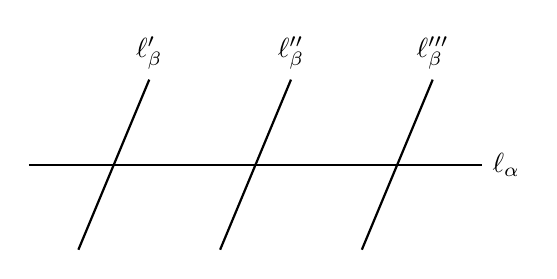
\begin{tikzpicture}[scale=0.9]
\draw[thick] (-3.2,0) -- (3.2,0) node[right] {$\ell_\alpha$};
\foreach \x/\l in {-2/{\ell_\beta'},0/{\ell_\beta''},2/{\ell_\beta'''}}
  {\draw[thick] (\x-0.5,-1.2) -- (\x+0.5,1.2) node[above] {$\l$};}
\end{tikzpicture}
\caption{The Dynkin curve of a subregular unipotent element of $G_2$, drawn
from the description in the text.}\label{fig:dynkin}
\end{figure}

\begin{rem26}\label{rem:dynkin}
The figure of the Dynkin curve is missing from the 1994 source (the source
has empty displays). Figure~\ref{fig:dynkin} is reconstructed from the
description of the Galois actions below. The assignment of the types
$\alpha$ and $\beta$ to the central and outer lines is taken from that
description and has not been checked against \cite{St74}.
\end{rem26}

Possible Galois actions on this configuration include:
(i) exchanging $\ell_\beta'$ with $\ell_\beta'''$, fixing
$\ell_\beta''$, and flipping $\ell_\alpha$;
(ii) flipping $\ell_\beta'$, $\ell_\beta''$, $\ell_\beta'''$
and fixing $\ell_\alpha$;
(iii) cyclically permuting $\ell_\beta'$, $\ell_\beta''$, $\ell_\beta'''$
and ``rotating'' $\ell_\alpha$.

Label and order the positive roots of the maximal torus
$T_+\subset B_-$ of $G_2$ as
\[
\alpha \text{ (short)},\ \beta \text{ (long)},\
\gamma=\alpha +\beta,\ \delta =2\alpha +\beta,\
\epsilon =3\alpha +\beta,\  \zeta=3\alpha +2\beta .
\]
We have
\[
\theta_\delta(r)\theta_\gamma(s)=\theta_\gamma(s)\theta_\delta(r)\theta_{\zeta}(3rs),
\]
up to the sign of the structure constant, so
\[
\begin{split}
\theta_{\eps}(x)^{\theta_{-\alpha}(z)}
&=\theta_{\eps}(x)\theta_\delta(c_1xz)\theta_\gamma(c_2xz^2)
\theta_\beta(c_3xz^3)\\
&=\theta_\beta(c_3xz^3)\theta_\gamma(c_2xz^2)\theta_\delta(c_1xz)\theta_{\eps}(x)
\theta_\zeta(c_4x^2z^3),
\end{split}
\]
where the $c_i$ are constants determined by the Chevalley basis. Likewise,
\[
\theta_{\delta}(x)^{\theta_{-\alpha}(z)}
=\theta_\beta(d_2xz^2)\theta_\gamma(d_1xz)\theta_{\delta}(x)\theta_\zeta(d_3x^2z),
\]
\[
\theta_{\gamma}(x)^{\theta_{-\alpha}(z)}
=\theta_{\gamma}(x)\theta_\beta(exz)=\theta_\beta(exz)\theta_{\gamma}(x),
\qquad
\theta_{\beta}(x)^{\theta_{-\alpha}(z)}=\theta_{\beta}(x),
\]
and, by a computation in $SL(2)$,
\[
\theta_{\alpha}(x)^{\theta_{-\alpha}(z)}=
\theta_{-\alpha}\Big(\frac{-xz^2}{1+xz}\Big)\,\alpha^\vee(1+xz)\,
\theta_{\alpha}\Big(\frac{x}{1+xz}\Big).
\]

In general, if $\sigma\in\Gamma$ acts on
$T_G(\overline{F})$ as a simple
reflection $s_\rho$, $\rho\in\Delta$, we write $\sigma=\sigma_\rho$.
This amounts to taking $\sigma(n_{\sigma_T^{-1}(W_0)})=\theta_{-\rho} (z)$,
where $z=\sigma(z(\rho)z_1(W_0,\rho))$ \cite[\S 3]{Ha89}. We
compute the Galois action on the coordinates of a point $P$ in
$Y''(B_+,B_-)$, assuming that $B_+\cap B_-=T_+$ is defined over
$F$ and $c_\sigma =1$ in \eqref{eq:2.9}. (Reflections $c_\sigma$ are treated
in \eqref{eq:2.16}--\eqref{eq:2.17}.)

Take $\sigma=\sigma_\alpha$, and order the product with $\alpha$ first. Then
\begin{equation}\tag{2.11}\label{eq:2.11}
\prod_{\rho >0}\theta_\rho(x(\rho))^{\theta_{-\alpha}(z)}
=\theta_{-\alpha}(y_\alpha)
t\prod_{\rho >0}\theta_\rho(\phi_\rho^\alpha(\unx,z)),
\end{equation}
with $t=\alpha^\vee(1+x(\alpha)z)$, $y_\alpha=-x(\alpha)z^2/(1+x(\alpha)z)$,
$\unx =(x(\alpha),\dots, x(\zeta))$, and, up to conjugation of the factors
$\theta_\rho$, $\rho\neq\alpha$, by $t$,
\[
\begin{split}
\phi_\alpha^\alpha(\unx,z)
&=x(\alpha)/(1+x(\alpha)z),\\
\phi_\beta^\alpha(\unx,z)
&=x(\beta)+ezx(\gamma)+d_2z^2x(\delta)+c_3z^3x(\eps),\\
\phi_\gamma^\alpha(\unx,z)
&=x(\gamma)+d_1zx(\delta)+c_2z^2x(\eps),\\
\phi_\delta^\alpha(\unx,z)
&=x(\delta)+c_1zx(\eps),\\
\phi_{\eps}^\alpha(\unx,z)
&=x(\eps),\\
\phi_\zeta^\alpha(\unx,z)
&=x(\zeta)+d_3zx(\delta)^2+c_4z^3x(\eps)^2+\text{(cross terms in }x(\delta)x(\eps)).
\end{split}
\]
Therefore, if $c_{\sigma_\alpha}=1$, we have
\begin{equation}\tag{2.12}\label{eq:2.12}
\sigma_\alpha :x(\rho)\longmapsto \sigma\big(\phi_\rho^\alpha(\unx,z)\big),
\end{equation}
where $z=\sigma_\alpha(z(\alpha)z_1(W_0,\alpha))$.

\begin{rem26}[formulas \eqref{eq:2.11}--\eqref{eq:2.14}]\label{rem:2.11}
These formulas are schematic. The constants are not computed, and the
reordering of the factors produces further cross terms that are not written
out. Several misprints of 1994 are corrected:
\begin{itemize}
\item $\phi^\alpha_\alpha=x(\alpha)$ is replaced by $x(\alpha)/(1+x(\alpha)z)$,
from the $SL(2)$ computation above, and the torus factor $t$, which rescales
the other coordinates, is recorded;
\item the analogous $y_\beta$ is $-xz^2/(1+xz)$, not $-x^2z/(1+xz)$;
\item in $\phi^\alpha_\delta$, $c_2$ is replaced by $c_1$;
\item in the commutator of $\theta_\beta(r)$ and $\theta_\alpha(s)$ the
exponents were interchanged, because the root $i\alpha+j\beta$ carries $s^ir^j$;
\item after Lemma~\ref{res:2.10}, $\theta_\rho(z)$ is replaced by
$\theta_{-\rho}(z)$.
\end{itemize}
With the normalization of Remark~\ref{rem:2.8}, $b'=m_\sigma\sigma(b)m_\sigma^{-1}
=\sigma(b)^{\theta_{-\alpha}(-z)}$, so $z$ should be read as $-z$ in
\eqref{eq:2.11}--\eqref{eq:2.14}. The formulas were not used in a computation in 1994, and they are not used in
one here.
\end{rem26}

Take $\sigma =\sigma_\beta$ and note
\[
\theta_\gamma(r)\theta_\alpha (s)=\theta_\alpha (s)\theta_\gamma(r)
\theta_\delta(2rs)\theta_\epsilon(3rs^2)\theta_\zeta(3r^2s),
\]
\[
\theta_\beta(r)\theta_\alpha (s)=\theta_\alpha (s)\theta_\beta(r)
\theta_\gamma(rs)
\theta_\delta(rs^2)\theta_\epsilon(rs^3)\theta_\zeta(r^2s^3),
\]
up to the signs of the structure constants.
By Chevalley's commutator formula,
\[
\theta_\alpha(x)^{\theta_{-\beta}(z)}=\theta_\alpha(x),\qquad
\theta_\beta(x)^{\theta_{-\beta}(z)}=
\theta_{-\beta}(y_\beta)\,
\beta^\vee(1+xz)\,\theta_\beta\Big(\frac{x}{1+xz}\Big),\quad
y_\beta:={-xz^2\over 1+xz},
\]
\[
\theta_\gamma(x)^{\theta_{-\beta}(z)}
=\theta_\gamma(x)\theta_\alpha(czx)
=\theta_\alpha(czx)\theta_\gamma(x)\theta_\delta(2czx^2)
\theta_\epsilon(3c^2z^2x^3)\theta_\zeta(3czx^3),
\]
\[
\theta_\delta(x)^{\theta_{-\beta}(z)}=\theta_\delta(x),\qquad
\theta_\epsilon(x)^{\theta_{-\beta}(z)}=\theta_\epsilon(x),\qquad
\theta_\zeta(x)^{\theta_{-\beta}(z)}=\theta_\zeta(x)\theta_\epsilon(dzx)
=\theta_\epsilon(dzx)\theta_\zeta(x).
\]
Therefore
\begin{equation}\tag{2.13}\label{eq:2.13}
\prod_{\rho >0}\theta_\rho(x(\rho))^{\theta_{-\beta}(z)}
=\theta_{-\beta}(y_\beta)\,t\prod_{\rho >0}\theta_\rho(\phi_\rho^\beta(\unx,z)),
\end{equation}
where, schematically,
\[
\begin{split}
\phi_\alpha^\beta(\unx,z)
&=x(\alpha)+cx(\gamma)z+\cdots,\\
\phi_\beta^\beta(\unx,z)
&=x(\beta)/(1+x(\beta)z),\\
\phi_\gamma^\beta(\unx,z)
&=x(\gamma)+\cdots,\\
\phi_\delta^\beta(\unx,z)
&=x(\delta)+2czx(\gamma)^2+\cdots,\\
\phi_{\eps}^\beta(\unx,z)
&=x(\eps)+dzx(\zeta)+3c^2x(\gamma)^3z^2+\cdots,\\
\phi_\zeta^\beta(\unx,z)
&=x(\zeta)+3czx(\gamma)^3+\cdots.
\end{split}
\]
Therefore, if $c_{\sigma_\beta}=1$, we have
\begin{equation}\tag{2.14}\label{eq:2.14}
\sigma_\beta :x(\rho)\longmapsto \sigma\big(\phi_\rho^\beta(\unx,z)\big),
\end{equation}
where $z=\sigma_\beta(z(\beta)z_1(W_0,\beta))$.

Formulas \eqref{eq:2.12} and \eqref{eq:2.14} help to determine the set of
$F$-rational points of $Y_C$. We also need the effect of conjugating $b$ by
$c_\sigma$. For this we recall a basic lemma \cite{Ca89}.

\begin{res}{Lemma}{2.15}\label{res:2.15}
Let $\phi_\rho:SL(2)\rightarrow G$ be the
homomorphism associated to the root
$\rho$ and let $\theta_\rho:\gga_a\rightarrow U_\rho$ denote the root
group embedding, so
$\theta_\rho(x)=\phi_\rho\big(\begin{smallmatrix} 1&x\\ 0&1\end{smallmatrix}\big)$.
Let $s_\rho:=s_\rho(1)$, where
\[
s_\rho(x)=\theta_\rho(x)\theta_{-\rho}(-x^{-1})\theta_\rho(x)
=\phi_\rho\begin{pmatrix} 0&x\\ -1/x&0\end{pmatrix}.
\]
Then
$s_\rho \theta_\sigma (x)s_\rho^{-1}
=\theta_{w_\rho(\sigma)}(\eta_{\rho,\sigma}x)$,
where $\eta_{\rho,\sigma}=\pm1$ is as in \cite[pp.~94--96]{Ca89} and $w_\rho$ is
the reflection of the Weyl group associated to $\rho$.
\end{res}

As a consequence,
\begin{equation}\tag{2.16}\label{eq:2.16}
s_\alpha\cdot \prod_{\rho>0}\theta_{\rho}(x(\rho))\cdot s_\alpha^{-1}
=\theta_{-\alpha}(x'(\alpha))
\prod_{\rho>0, \rho\not=\alpha}\theta_{\rho}(x'(\rho)),
\end{equation}
where $x'(\alpha)=\eta_{\alpha,\alpha}x(\alpha)$,
$x'(\beta)=\eta_{\alpha,\epsilon}x(\epsilon)$,
$x'(\gamma)=\eta_{\alpha,\delta}x(\delta)$,
$x'(\delta)=\eta_{\alpha,\gamma}x(\gamma)$,
$x'(\epsilon)=\eta_{\alpha,\beta}x(\beta)$,
and
$x'(\zeta)=\eta_{\alpha,\zeta}x(\zeta)+
f_1x(\delta)x(\gamma)+f_2x(\beta)x(\epsilon)$,
where $f_1,f_2$ are constants. Likewise,
\begin{equation}\tag{2.17}\label{eq:2.17}
s_\beta\cdot \prod_{\rho>0}\theta_{\rho}(x(\rho))\cdot s_\beta^{-1}
=\theta_{-\beta}(x'(\beta))
\prod_{\rho>0, \rho\not=\beta}\theta_{\rho}(x'(\rho)),
\end{equation}
where
$x'(\alpha)=\eta_{\beta,\gamma}x(\gamma)+f_3x(\alpha)x(\beta)$,
$x'(\beta)=\eta_{\beta,\beta}x(\beta)$,
$x'(\gamma)=\eta_{\beta,\alpha}x(\alpha)$,
$x'(\delta)=\eta_{\beta,\delta}x(\delta)+f_4x'(\alpha)x'(\gamma)$,
$x'(\epsilon)=\eta_{\beta,\zeta}x(\zeta)$, and
$x'(\zeta)=\eta_{\beta,\epsilon}x(\epsilon)$.
These follow from $s_\alpha$: $\beta\mapsto\epsilon$, $\gamma\mapsto\delta$,
$\delta\mapsto\gamma$, $\epsilon\mapsto\beta$, $\zeta\mapsto\zeta$, and
$s_\beta$: $\alpha\mapsto\gamma$, $\gamma\mapsto\alpha$, $\delta\mapsto\delta$,
$\epsilon\mapsto\zeta$, $\zeta\mapsto\epsilon$ (checked, level 1). The
reordering needed to move $\theta_{-\alpha}$ (respectively $\theta_{-\beta}$)
to the front produces further terms, which are not written out. In 1994 the
signs in \eqref{eq:2.17} were written $\eta_{\alpha,\cdot}$.
% =====================================================================
% Section 3. Source: g2new3.tex.
% =====================================================================
\numsection{3}{Construction of regular patches}\label{sec:3}

This section describes the local structure of $Y''$. Locally it is the
product of an affine space with a monomial variety $Z$, an affine toric
variety. We introduce the fundamental and essential patches of $Z$, prove
that for $G_2$ they are regular and cover $Z$ up to codimension two, and
prove that $Z$ is normal and Cohen--Macaulay for $G_2$.

Let $G$ denote a connected semisimple group over $\ovF$.
Let $\chi:G\rightarrow T_G/\Omega$ denote the adjoint quotient \cite{Sl80}.
There is an open patch
\[
Y''(B_+,B_-)\times N_+\subset
\chi^{-1}(C)\times S''(B_+,B_-)\times N_+
\subset G\times S''(B_+,B_-)\times N_+
\]
of $Y''$ which is isomorphic to an open subset of the product
$\aaa^p\times Z$, where $Z\subset \aaa^{2p+1}$ is the
``monomial'' affine variety of dimension $p+1$ with coordinates
\[
w(\rho)\ (\rho\in \Sigma_G^+ -\Delta),\qquad
z(\alpha)\ (\alpha\in\Delta),\qquad x(\rho)
\ (\rho\in\Sigma_G^+),\qquad \lambda,
\]
defined as the Zariski closure of the set of points with $\lambda\neq0$
satisfying, for all $\rho\in\Sigma_G^+$,
\begin{equation}\tag{3.1}\label{eq:3.1}
\lambda w(\rho )=x(\rho)\prod_{\alpha\in\Delta }z(\alpha )^{m(\alpha)},
\end{equation}
where we set $w(\alpha)=1$ for $\alpha\in\Delta$, and $m(\alpha)=m_\rho(\alpha)\geq 0$ is the coefficient of $\alpha$ in
$\rho = \sum_{\alpha\in\Delta }m(\alpha)\alpha $.
Here $\Delta$ denotes the simple roots of $T_+$ in $B_-$.
In particular $\lambda =x(\alpha)z(\alpha)$ for $\alpha$ simple.
On $\lambda\neq0$ the coordinates $\lambda$, $z(\alpha)$ ($\alpha\in\Delta$),
and $w(\rho)$ ($\rho\notin\Delta$) are free, the $z(\alpha)$ are non-zero, and
the $x(\rho)$ are determined by \eqref{eq:3.1}. So $Z$ is the closure of the
orbit of a torus of dimension $p+1$: it is the affine toric variety
$\operatorname{Spec}k[S]$, where $S$ is the semigroup of exponent vectors of the
monomials $\lambda$, $z(\alpha)$, $w(\rho)$, $x(\rho)$ in the torus coordinates
$(\lambda,z(\alpha),w(\rho))$. The projection of the patch onto $Z$ lets us
pull back open subvarieties $Z_U\subset Z$ to open subvarieties
$Y''_U\subset Y''$. The variety $Z$ is regular on $\lambda\neq0$.

\begin{example}
For $G_2$, $p=6$, $Z\subset\aaa^{13}$ has dimension $7$, and the torus
coordinates are $\lambda,z(\alpha),z(\beta),w(\gamma),w(\delta),w(\epsilon),
w(\zeta)$. For instance $x(\zeta)=\lambda w(\zeta)z(\alpha)^{-3}z(\beta)^{-2}$,
so the exponent vector of $x(\zeta)$ is $(1,-3,-2,0,0,0,1)$.
\end{example}

We first claim that, for $G=G_2$,
the singularities of $Z$ lie in
\[
K:\quad x(\alpha)=x(\beta)=x(\gamma)=z(\alpha)=w(\zeta)=0
\]
or in
\[
K_0:\quad x(\alpha)=x(\beta)=x(\gamma)=x(\delta)=x(\epsilon)=x(\zeta)=w(\zeta)=0.
\]
The points of $Y''(B_+,B_-)$ with coordinates in $K_0$ have $\lambda=0$ and
map to the identity under $\pi$, hence correspond to the trivial class.
To prove the claim, we exhibit four regular patches, give generators of the
local coordinate ring, and express the remaining coordinates as regular
functions of the generators on the patch.

\medskip\noindent
$x(\alpha)\not= 0$. Generators: $x(\alpha)$, $x(\beta)$, $z(\beta)$, $x(\gamma)$,
$x(\delta)$, $x(\epsilon)$, $x(\zeta)$. Remaining coordinates:
$\lambda=x(\beta)z(\beta)$, $z(\alpha)=x(\beta)z(\beta)/x(\alpha)$,
$w(\gamma)=x(\gamma)z(\beta)/x(\alpha)$,
$w(\delta)=x(\delta)z(\alpha)z(\beta)/x(\alpha)$,
$w(\epsilon)=x(\epsilon)z(\alpha)^2 z(\beta)/x(\alpha)$,
$w(\zeta)=x(\zeta)z(\alpha)^2 z(\beta)^2 /x(\alpha)$.

\medskip\noindent
$x(\beta)\not= 0$. Generators: $x(\alpha)$, $x(\beta)$, $z(\alpha)$, $x(\gamma)$,
$x(\delta)$, $x(\epsilon)$, $x(\zeta)$. Remaining coordinates:
$\lambda=x(\alpha)z(\alpha)$, $z(\beta)=x(\alpha)z(\alpha)/x(\beta)$,
$w(\gamma)=x(\gamma)z(\alpha)/x(\beta)$,
$w(\delta)=x(\delta)z(\alpha)^2 /x(\beta)$,
$w(\epsilon)=x(\epsilon)z(\alpha)^3 /x(\beta)$,
$w(\zeta)=x(\zeta)x(\alpha)z(\alpha)^4 /x(\beta)^2$.

\medskip\noindent
$x(\gamma)\not= 0$. Generators: $x(\alpha)$, $x(\beta)$, $x(\gamma)$, $w(\gamma)$,
$x(\delta)$, $x(\epsilon)$, $x(\zeta)$. Remaining coordinates:
$\lambda=x(\alpha)x(\beta)w(\gamma)/x(\gamma)$,
$z(\alpha)=x(\beta)w(\gamma)/x(\gamma)$, $z(\beta)=x(\alpha)w(\gamma)/x(\gamma)$,
$w(\delta)=x(\delta)w(\gamma)^2 x(\beta)/x(\gamma)^2$,
$w(\epsilon)=x(\epsilon)w(\gamma)^3 x(\beta)^2 /x(\gamma)^3$,
$w(\zeta)=x(\zeta)x(\alpha) x(\beta)^2 w(\gamma)^4 /x(\gamma)^4$.

\medskip\noindent
$w(\zeta)\not= 0$. Generators: $z(\alpha)$, $z(\beta)$, $w(\gamma)$,
$w(\delta)$, $w(\epsilon)$, $w(\zeta)$, $x(\zeta)$. Remaining coordinates:
$\lambda=x(\zeta)z(\alpha)^3 z(\beta)^2 /w(\zeta)$,
$x(\alpha)=x(\zeta)z(\alpha)^2 z(\beta)^2 /w(\zeta)$,
$x(\beta)=x(\zeta)z(\alpha)^3 z(\beta) /w(\zeta)$,
$x(\gamma)=w(\gamma)x(\zeta) z(\alpha)^2 z(\beta) /w(\zeta)$,
$x(\delta)=w(\delta)x(\zeta) z(\alpha) z(\beta) /w(\zeta)$,
$x(\epsilon)=w(\epsilon)x(\zeta)z(\beta) /w(\zeta)$.

\medskip
On $Z$ the monomial identities $x(\delta)z(\alpha)^2=x(\beta)w(\delta)$,
$x(\epsilon)z(\alpha)^3=x(\beta)w(\epsilon)$ and
$x(\zeta)z(\alpha)^3z(\beta)=x(\beta)w(\zeta)$ hold, because both sides are
the same character of the torus. Hence, if $x(\alpha)=x(\beta)=x(\gamma)=w(\zeta)=0$
and $z(\alpha)\neq0$, then also $x(\delta)=x(\epsilon)=x(\zeta)=0$. So the
complement of the four patches is contained in $K\cup K_0$, and the claim
follows.

\begin{rem26}\label{rem:3.patches}
Three of the patch formulas were misprinted in 1994. The correct values are
$w(\zeta)=x(\zeta)x(\alpha)z(\alpha)^4/x(\beta)^2$ on $x(\beta)\neq0$ and
$w(\zeta)=x(\zeta)x(\alpha)x(\beta)^2w(\gamma)^4/x(\gamma)^4$ on
$x(\gamma)\neq0$; the 1994 versions were $x(\zeta)z(\alpha)^5x(\alpha)^2/x(\beta)^3$
and $x(\zeta)x(\alpha)x(\beta)^2w(\gamma)^4/x(\gamma)$. The 1994 text also
gave a fifth patch, $z(\alpha)\neq0$ with $x(\epsilon)\neq0$ (or
$x(\delta)\neq0$, or $x(\zeta)\neq0$). By the identities above it lies inside
$\{x(\beta)\neq0\}$, so it is omitted; its formula for $w(\zeta)$ had a
spurious factor $z(\alpha)^{-3}$. All formulas were checked symbolically
(script \texttt{g2\_patch\_jacobians.py}).
\end{rem26}

The claim is weaker than it looks: $K$ contains the divisor
$E_{\emptyset,\alpha,\delta}$ of \S\ref{sec:4}, along which $Z$ is
generically regular. The exact singular locus is described in
Remark~\ref{rem:exceptional}. Since $Z$ is a normal toric variety
(Proposition~\ref{res:3.7}), it has a resolution of singularities
$\tilde Z\to Z$ given by a regular subdivision of its fan, which is an
isomorphism over the regular locus. The divisor $\lambda=0$ in $\tilde Z$ has
normal crossings, but its branches occur with multiplicities $a(E)$ that may
exceed $1$ (Table~\ref{tab:4.3A}). Let $\tilde{Y''}\rightarrow Y''$ be the
corresponding resolution of $Y''$. The exceptional divisors of
$\tilde{Y''}\to Y''$ have not been analyzed (Remark~\ref{rem:exceptional}).

\subsection*{Fundamental and essential patches}

Let $G$ again be an arbitrary connected semisimple group.
Let $\Delta=\{\alpha_1,\dots,\alpha_\ell\}$, which we sometimes identify
with $\{1,\dots,\ell\}$, $\ell :=\mathrm{rk}\, G$. Let $S_1,S_2\subset \{1,\dots,\ell\}$
be disjoint sets. If they are
non-empty, let $i_{min}:=\min_{i\in S_1}i$,
$j_{min}:=\min_{j\in S_2}j$, and similarly $i_{max},\ j_{max}$. If
$S_1,S_2$ are non-empty, we assume
(i) $i_{max}<j_{min}$ or $j_{max}<i_{min}$, and (ii) if $S_2\not=\emptyset$
then $S_1\cup S_2\not=\Delta$.

For each map $\sigma :S_2 \rightarrow \Sigma_G^+ -\Delta$,
define the subset $Z_{S_1,S_2,\sigma}\subset Z$ by the conditions
\begin{enumerate}[label=(3.2\alph*)]
\item\fixedlabel{3.2a}\label{eq:3.2a} $z(\alpha)\not= 0$ for all $\alpha\notin S_1\cup S_2$,
\item\fixedlabel{3.2b}\label{eq:3.2b} $x(\alpha)\not= 0$ for all $\alpha\in S_1$,
\item\fixedlabel{3.2c}\label{eq:3.2c} $x(\sigma(j))\not= 0$ for all $j\in S_2$,
\item\fixedlabel{3.2d}\label{eq:3.2d} $w(\sigma(j))\not= 0$ for all $j\in S_2$.
\end{enumerate}
These are the \textbf{fundamental patches} of $Z$ in the sense of \cite{Ha92a}.
The collection depends, a priori, on the
identification of $\Delta$ with $\{1,\dots,\ell\}$.
For $G=G_2$ the divisor $\lambda =0$ meets each
$Z_{S_1,S_2,\sigma}$ in a single irreducible branch, denoted
$E_{S_1,S_2,\sigma}$, occurring with some multiplicity
$a(E_{S_1,S_2,\sigma})$ (Table~\ref{tab:4.3A}).
The $E_{S_1,S_2,\sigma}$ are the \textbf{fundamental branches} of
$\lambda =0$ on $Z$. If $S_2=\{\rho\}$ is a singleton and
$\tau=\sigma(\rho)$, we write $E_{S_1,\rho,\tau}$ for $E_{S_1,S_2,\sigma}$.
If $S_2 =\emptyset$ we write
$Z_{S_1}$ and call it a \textbf{Richardson patch}, and
$E_{S_1}$ a \textbf{Richardson branch},
since by \cite[Ch.~II, Proposition~9.1]{Ha92a}
$\pi(E_{S_1})$ is the closure of the Richardson class of the parabolic
subgroup $P_{\Delta-S_1}$ whose Levi subgroup has simple roots $\Delta-S_1$.
In particular the \textbf{regular branch} is $E_\Delta$ ($S_1=\Delta$),
with $\pi(E_\Delta)=\overline{\mathcal O}_{reg}=V$, the unipotent variety,
and $E_\emptyset$ is the branch of the trivial class. Since
$E_\Delta$ is regular,
$\pi:E_\Delta \rightarrow V$ is a resolution of singularities
similar to the Springer resolution \cite{Sl80}, \cite{St74}.

\begin{rem26}\label{rem:3.regular-branch}
The 1994 text called $E_\emptyset$ the regular branch. With the convention
of this paper (``Hales' $E_S$ is my $E_{\Delta -S}$'') the regular branch is
$E_\Delta$; $E_\emptyset$ maps to the identity (Table~\ref{tab:4.3A}).
\end{rem26}

Fix a map $\sigma :S_2 \rightarrow \Sigma_G^+ -\Delta$ satisfying the
following.
\begin{enumerate}[label=(3.3\alph*)]
\item\fixedlabel{3.3a}\label{eq:3.3a} For $j,j'\in S_2$, the simple root expansions of $\sigma(j)$ and
$\sigma(j')$ contain no common simple roots unless $j=j'$ or
$j,j'$ are consecutive.
\item\fixedlabel{3.3b}\label{eq:3.3b} If $j,j'$ are consecutive in $S_2$ then
$\sigma(j)=\sum_{k=j}^{j'}m_{jk}\alpha_k$
for some integers $m_{jk}\geq 0$.
\item\fixedlabel{3.3c}\label{eq:3.3c} There is an $a\geq 1$ for which $\sigma(j_{max})
=a\alpha_{j_{max}}+\sum_{\alpha\notin S_1\cup S_2}m(\alpha)\alpha$,
for some integers $m(\alpha)\geq 0$.
\end{enumerate}
Such a map, and the corresponding fundamental patch, are called
\textbf{essential}. Patches which are not essential are expected to be
redundant in a covering of $Z$ up to codimension $2$, but in general there
are also redundant essential patches, so the definition is provisional.
These patches generalize the
sequences $\gamma(i,j),\dots$ of roots used in \cite{Ha89}.

\begin{resdef}{Notation}{3.3d}\label{res:notation}
The notation for these divisors differs from that of \cite{Ha92a},
\cite{Ha89}, though the notation for the patches seems to agree:
Hales' $E_S$ is our $E_{\Delta -S}$.
\end{resdef}

\begin{res}{Conjecture}{3.4}\label{res:3.4}
If $G$ is not of type $D_n$, $E_n$, $F_4$, then
$Z$ is covered by the essential patches $Z_{S_1,S_2,\sigma}$ except for
a subset of codimension $\geq 2$, and the $Z_{S_1,S_2,\sigma}$
are all regular.
\end{res}

\begin{rem26}\label{rem:3.4}
The 1994 manuscript stated that Conjecture~\ref{res:3.4} ``is known'' for
$A_n$ and $C_n$ \cite{Ha92a}, \cite{Ha89}, and false for $D_n$. These claims
have not been checked; \cite{Ha89} treats only $GSp(4)$. The 1994 statement
also included ``$Z$ is regular in codimension one''; that holds for every $G$
for which $Z$ is normal (Proposition~\ref{res:3.7} and
Conjecture~\ref{res:3.7A}).
\end{rem26}

\begin{res}{Proposition}{3.4A}\label{res:3.4A}
Conjecture~\ref{res:3.4} holds for $G_2$. More precisely, the twelve patches
listed in \S\ref{sec:4} are regular, with the generators given there, and
every torus-invariant prime divisor of $Z$ meets one of them.
\end{res}

\begin{proof}
Regularity: on each patch, every coordinate of $Z$ is a monomial in the
listed generators, with negative exponents only on generators that are
inverted on the patch; this was checked symbolically for all twelve patches
(script \texttt{g2\_patch\_regularity.py}). Covering: the complement of a
union of torus-invariant open sets is torus-invariant and closed, so it has
codimension at least $2$ unless it contains a torus-invariant prime divisor.
For a facet of the cone of $S$ with primitive inner normal $u$, the patch
$\{m\neq0\}$ meets the divisor $D_u$ exactly when $\langle m,u\rangle=0$.
The eleven facets of the cone were computed, and each is orthogonal to the
monomial of at least one patch (script \texttt{g2\_toric\_divisors.py}).
\end{proof}

\begin{res}{Lemma}{3.5}[Hales \cite{Ha92a}, corrected]\label{res:3.5}
For $S_1\subset \Delta$ non-empty, $Z_{S_1}$ is regular, with
generators
\[
\lambda,\quad z(\alpha)\ (\alpha\in\Delta -S_1),\quad
x(\rho)\ (\rho\in\Sigma_G^+-\Sigma_{\Delta-S_1}^+),\quad
w(\rho)\ (\rho\in \Sigma_{\Delta-S_1}^+-\Delta),
\]
where $\Sigma_{\Delta-S_1}^+$ denotes the positive roots of the
root subsystem spanned by $\Delta-S_1$. (The $x(\rho)$ include
$x(\alpha)$ for $\alpha\in S_1$.) It is
$(p+1)$-dimensional, and the divisor $\lambda =0$ occurs on it with
multiplicity one.
\end{res}

\begin{proof}
On $Z_{S_1}$ we have $z(\alpha)=\lambda/x(\alpha)$ for $\alpha\in S_1$. For a
positive root $\rho$ write $m_{S_1}(\rho)=\sum_{\alpha\in S_1}m_\rho(\alpha)$.
By \eqref{eq:3.1},
\[
w(\rho)=x(\rho)\,\lambda^{m_{S_1}(\rho)-1}\prod_{\alpha\notin S_1}
z(\alpha)^{m_\rho(\alpha)}\prod_{\alpha\in S_1}x(\alpha)^{-m_\rho(\alpha)}.
\]
If $\rho\notin\Sigma^+_{\Delta-S_1}$ then $m_{S_1}(\rho)\geq1$, and $w(\rho)$
is regular in $x(\rho)$ and the generators. If $\rho\in\Sigma^+_{\Delta-S_1}$
then $m_{S_1}(\rho)=0$ and $x(\rho)=\lambda w(\rho)\prod_{\alpha\notin
S_1}z(\alpha)^{-m_\rho(\alpha)}$ is regular in $w(\rho)$ and the generators.
So all coordinates are regular functions of the listed ones, whose number is
$1+(\ell-|S_1|)+(p-|\Sigma^+_{\Delta-S_1}|)+(|\Sigma^+_{\Delta-S_1}|-(\ell-|S_1|))
=p+1=\dim Z$. Hence $Z_{S_1}$ is an open subset of affine space, with $\lambda$
one of the coordinates.
\end{proof}

\begin{rem26}\label{rem:3.5}
As printed in 1994, the lemma had $\Sigma^+_{S_1}$ in place of
$\Sigma^+_{\Delta-S_1}$, so the roles of $x(\rho)$ and $w(\rho)$ were
interchanged. For $S_1=\Delta$ that version gives the generators $\lambda$,
$x(\alpha)$, $x(\beta)$, $w(\gamma),\dots$, for which
$x(\gamma)=w(\gamma)x(\alpha)x(\beta)/\lambda$ is not regular. The generator
count also failed unless $S_1=\Delta$. The proof above is new.
\end{rem26}

For brevity, let $m_\alpha$ denote the multiplicity with
which $z(\alpha)=0$ occurs in $\lambda =0$.

\begin{res}{Lemma}{3.6}\label{res:3.6}
Let $\alpha\in\Delta$ and
$\sigma\in\Sigma_G^+ -\Delta$, and suppose that
$Z_{\emptyset,\alpha,\sigma}$ is an essential patch and that every positive
root is comparable with $\sigma$ in the partial order $\rho\le\sigma$ iff
$\sigma-\rho$ is a non-negative combination of simple roots. Then
$Z_{\emptyset,\alpha,\sigma}$ is regular and its coordinate ring has
generators
\[
z(\beta )\ (\beta\in\Delta ),\qquad
x(\rho)\ (\rho \geq\sigma),\qquad
w(\rho)\ (\rho \leq \sigma,\ \rho\notin\Delta).
\]
The divisor $\lambda =0$ occurs as $z(\alpha)=0$
with multiplicity $m$, where $m\geq 1$ is the coefficient of
$\alpha$ in $\sigma$. The hypothesis holds for $G_2$.
\end{res}

\begin{proof}
Write $\sigma=m\alpha +\sum_{\beta\not= \alpha}m_\beta\beta$. On
$Z_{\emptyset,\alpha,\sigma}$ we have $z(\beta)\not= 0$
for $\beta\not=\alpha$ simple, $x(\sigma)\not= 0$, and
$w(\sigma)\not= 0$. By \eqref{eq:3.3c} and \eqref{eq:3.1},
$\lambda
=x(\sigma)w(\sigma)^{-1}z(\alpha)^m\prod_{\beta\not= \alpha}z(\beta)^{m_\beta}$,
so $\lambda=0$ is the divisor $z(\alpha)=0$
with multiplicity $m$.
If $\rho \leq\sigma$, say $\sigma=\rho +\sum_\beta n(\beta)\beta$ with
$n(\beta)\ge0$, then
\[
x(\rho)={x(\sigma)w(\rho)\over w(\sigma)}
\prod_\beta z(\beta)^{n(\beta)},
\]
which is regular in the $w(\rho)$ with $\rho \leq\sigma$.
If $\rho\geq\sigma$ then
\[
w(\rho)={w(\sigma)x(\rho)\over x(\sigma)}\prod_\beta
z(\beta)^{m_\rho(\beta)-m_{\sigma}(\beta)},
\]
with non-negative exponents, which is regular in the $x(\rho)$ with
$\rho \geq\sigma$. For simple $\beta$, $x(\beta)=\lambda/z(\beta)$ is regular
because $m\ge1$. The number of generators is $\ell+|\{\rho\ge\sigma\}|+
|\{\rho<\sigma\}|-\ell=p+1$ when every root is comparable with $\sigma$.
For $G_2$ the hypothesis is checked directly: $\delta-\gamma$, $\epsilon-\gamma$,
$\zeta-\gamma$, $\epsilon-\delta$, $\zeta-\delta$, $\zeta-\epsilon$ are all
non-negative combinations of $\alpha$ and $\beta$, and the simple roots are below
every non-simple root.
\end{proof}

\begin{rem26}\label{rem:3.6}
In 1994 the statement read ``$x(\rho)$ if $\rho>\sigma$'', while the proof
used $\rho\geq\sigma$; with $\rho>\sigma$ the generator count is one short.
The comparability hypothesis is new; without it the count fails in general,
since roots incomparable with $\sigma$ are not covered by either list.
\end{rem26}

\begin{res}{Proposition}{3.7}\label{res:3.7}
For $G=G_2$, the variety $Z$ is normal and Cohen--Macaulay.
\end{res}

\begin{proof}
$Z=\operatorname{Spec}k[S]$ is an affine toric variety. It is normal if and
only if $S$ is saturated in the lattice it generates \cite[Ch.~I, Theorem~1]{Ke72}.
For $G_2$ that lattice is $\zzz^7$, since the torus coordinates themselves
lie in $S$. Every generator of $S$ has degree $0$ or $1$ in $\lambda$. By
Carath\'eodory's theorem every lattice point of the cone of $S$ lies in a
simplicial subcone spanned by seven linearly independent generators, and is
the sum of a lattice point of the half-open fundamental parallelepiped of that
subcone and a non-negative integral combination of its generators. The
parallelepiped points have $\lambda$-degree at most $6$, and, since
$z(\alpha)$ and $z(\beta)$ are the only generators with a positive
$z$-coordinate, their $z$-coordinates are at most $0$; this confines them to
a finite set. So $S$ is saturated if every lattice point of the cone in that
finite set lies in $S$. This was checked exhaustively in exact integer
arithmetic (script \texttt{g2\_saturation\_full.py}): $658{,}651$ lattice
points of $\lambda$-degree $1$ to $6$, all in $S$. Normal semigroup rings are Cohen--Macaulay by Hochster's theorem
\cite{Ho72} (see also \cite[Ch.~I, Theorem~14]{Ke72}).
\end{proof}

\begin{res}{Conjecture}{3.7A}\label{res:3.7A}
For every connected semisimple group $G$, the variety $Z$ is normal (hence
Cohen--Macaulay, and regular in codimension one).
\end{res}

\begin{rem26}[Lemma~3.7 of 1994]\label{rem:3.7}
The 1994 manuscript stated Proposition~\ref{res:3.7} for every connected
semisimple group, and added that $Z$ is a set-theoretic complete intersection.
Its proof asserted that the semigroup is saturated without checking it; that
part is now Conjecture~\ref{res:3.7A}. The complete-intersection claim was
justified by counting the $p$ relations \eqref{eq:3.1}. Those relations do not
cut out $Z$: for $G_2$ they also vanish on the $10$-dimensional set
$\lambda=z(\alpha)=z(\beta)=0$. The claim is withdrawn.
\end{rem26}
% =====================================================================
% Section 4. Source: g2new4.tex.
% =====================================================================
\numsection{4}{Regularity of patches for $G=G_2$}\label{sec:4}

We now write all the patches of \S\ref{sec:3} down for $G_2$ and compute
the Igusa constants of the branches of $\lambda=0$. Recall
$\Sigma_G^+=\{\alpha,\beta,\gamma:=\alpha+\beta,\delta:=2\alpha +\beta,
\epsilon:=3\alpha +\beta,\zeta:=3\alpha +2\beta\}$, with
$\alpha$ short and $\beta$ long, so $p=6$ and $\dim Z=7$. We have variables
\begin{equation}\tag{4.1}\label{eq:4.1}
\begin{split}
&x(\alpha),x(\beta),
x(\gamma),x(\delta),x(\epsilon),x(\zeta),\\
&z(\alpha),z(\beta),
w(\gamma),w(\delta),w(\epsilon),w(\zeta),\\
&\lambda,
\end{split}
\end{equation}
subject to the relations \eqref{eq:3.1}.

With $B_+$ chosen as in \S\ref{sec:3}, we define $\omega_{Y''(B_+)}$ to be
the form
\[
\omega_{Y''(B_+)}=d\lambda
\wedge dx(\alpha)\wedge dx(\beta)
\wedge dx(\gamma)\wedge dx(\delta)\wedge dx(\epsilon)\wedge dx(\zeta)
\wedge dv,
\]
where $dv$ is an invariant form on $N_+$. We use it to compute the Igusa
constants $\beta$ as in \cite{Ha89}.

By Lemma~\ref{res:3.5}, the Richardson patches $Z_{S_1}$ are regular.
Since $S_1\cup S_2\not= \Delta$
if $S_2\not= \emptyset$, the remaining patches are those with
$S_1=\emptyset$ and either $S_2=\{\alpha\}$, $\sigma(\alpha)\in\{\gamma,
\delta,\epsilon,\zeta\}$, or $S_2=\{\beta\}$, $\sigma(\beta)\in\{\gamma,
\delta,\epsilon,\zeta\}$. (The 1994 text also allowed $\sigma(\alpha)=\alpha$
and $\sigma(\beta)=\beta$; with $w(\alpha)=w(\beta)=1$ these give the
Richardson patches $Z_{\{\alpha\}}$ and $Z_{\{\beta\}}$ again, intersected
with $z(\beta)\neq0$, respectively $z(\alpha)\neq0$.) By
Lemma~\ref{res:3.6} the generators of the local coordinate ring are as
follows; each patch is regular, and the branch of $\lambda=0$ on it is the
divisor $z(\alpha)=0$, respectively $z(\beta)=0$, with the multiplicity $a$
shown.

\medskip
\begin{center}
\renewcommand{\arraystretch}{1.15}
\begin{tabular}{@{}lll@{}}
\toprule
patch & generators & $a$\\
\midrule
$Z_{\emptyset,\alpha,\gamma}$, $Z_{\emptyset,\beta,\gamma}$ &
$z(\alpha), z(\beta), x(\gamma), w(\gamma), x(\delta), x(\epsilon), x(\zeta)$ & $1$, $1$\\
$Z_{\emptyset,\alpha,\delta}$, $Z_{\emptyset,\beta,\delta}$ &
$z(\alpha), z(\beta), w(\gamma), x(\delta), w(\delta), x(\epsilon), x(\zeta)$ & $2$, $1$\\
$Z_{\emptyset,\alpha,\epsilon}$, $Z_{\emptyset,\beta,\epsilon}$ &
$z(\alpha), z(\beta), w(\gamma), w(\delta), w(\epsilon), x(\epsilon), x(\zeta)$ & $3$, $1$\\
$Z_{\emptyset,\alpha,\zeta}$, $Z_{\emptyset,\beta,\zeta}$ &
$z(\alpha), z(\beta), w(\gamma), w(\delta), w(\epsilon), w(\zeta), x(\zeta)$ & $3$, $2$\\
\bottomrule
\end{tabular}
\end{center}
\medskip

The two patches on each line have the same generators but are different open
sets: $Z_{\emptyset,\alpha,\sigma}$ has $z(\beta)\neq0$ and
$Z_{\emptyset,\beta,\sigma}$ has $z(\alpha)\neq0$, by \eqref{eq:3.2a}.
Together with $Z_{\{\alpha,\beta\}}$, $Z_{\{\alpha\}}$, $Z_{\{\beta\}}$ and
$Z_\emptyset$ these are the twelve patches of Proposition~\ref{res:3.4A}.

There is redundancy among the branches. Comparing the valuations they define
(Table~\ref{tab:4.3A}) one finds
\[
E_{\emptyset,\beta,\gamma}=E_{\emptyset,\beta,\delta}=
E_{\emptyset,\beta,\epsilon}=E_{\{\beta\}},\qquad
E_{\emptyset,\alpha,\gamma}=E_{\{\alpha\}},\qquad
E_{\emptyset,\alpha,\epsilon}=E_{\emptyset,\alpha,\zeta}.
\]
So $\lambda=0$ has exactly seven irreducible branches on $Z$.

\begin{rem26}\label{rem:4.redundancy}
The 1994 text noted only the first set of identities. The multiplicity of
$E_{\emptyset,\alpha,\zeta}$ was correctly given as $3$, the coefficient of
$\alpha$ in $\zeta$.
\end{rem26}

We denote the branch of $\{\lambda =0\}\subset Z$
occurring in $Z_{S_1,S_2,\sigma}$ by $E_{S_1,S_2,\sigma}$. The same notation
will be used for the corresponding branch in $Y''_U$ and for its Zariski closure
in $Y_1$. To determine which of the $\kappa$-stable germs, if any,
the divisor $E_{S_1,S_2,\sigma}$
contributes to by Formula~\ref{res:0.6},
we must compute the Igusa constant
\begin{equation}\tag{4.2}\label{eq:4.2}
\beta(\tilde{E}_{S_1,S_2,\sigma})=
\frac{b(\tilde{E}_{S_1,S_2,\sigma})}{a(\tilde{E}_{S_1,S_2,\sigma})},
\end{equation}
where $\tilde{E}$ denotes the strict transform of $E$ in the
desingularized variety $Y_C$.

We record two observations regarding the Igusa constants $\beta(E)$.

\smallskip\noindent
(I) If $\phi:V\rightarrow W$ is an isomorphism of smooth varieties
which sends a divisor $E\subset V$ to a divisor $F=\phi(E)\subset W$,
then $\beta(E)=\beta(F)$.

\smallskip\noindent
(II) The numbers $a(E)=\mathrm{ord}_E(\lambda)$ and
$b(E)-1=\mathrm{ord}_E(\omega)$ depend only on the discrete valuation
$\mathrm{ord}_E$ of the function field, and $\omega$ is a rational top-degree
form. A birational morphism $\xi:V'\to V$ that is an isomorphism over the
generic point of $E$ does not change this valuation. Hence
$\beta(\tilde E)=\beta(E)$ for the strict transform $\tilde E$ of any branch
$E$ that meets the regular locus of $V$.

\begin{rem26}\label{rem:4.II}
The 1994 version of (II) used the blow-up formula
${\xi'}^*(E)=\tilde{E}+\delta E_{V'}$ and concluded that
$\beta(\tilde E)=\beta(E)$ ``provided $E$ does not contain any of the images
of the centers of the blow ups''. That proviso is unnecessary, by the
valuation argument above. Since $Z$ is normal (Proposition~\ref{res:3.7}),
every branch of $\lambda=0$ meets the regular locus of $Z$.
\end{rem26}

The only divisors in $\{\lambda =0\}\subset \tilde{Z}$ other than the strict
transforms $\tilde{E}$ above are exceptional divisors.
To compute all the $\beta$-values of the
branches of $\phi^{-1}(1)$ in $Y_C$ one must therefore compute the
$\beta$-values of the divisors $E_{S_1,S_2,\sigma}$ on $Z$ and of the
exceptional divisors of the resolution. The 1994 manuscript did not compute
the latter, on the grounds of Lemma~\ref{res:0.8} and the claim that all the
needed $F$-rational $\mathcal O$-divisors are among the $E_{S_1,S_2,\sigma}$.
That claim is the proviso of Lemma~\ref{res:0.8}; see
Remark~\ref{rem:exceptional}.

If $S_2=\emptyset$ then $\beta({E}_{S_1})$
has been computed in \cite[Ch.~II, Proposition~9.1]{Ha92a},
so some of our calculations are covered by Hales' general
calculations. For completeness, we list everything.

\subsection*{Igusa forms on the fundamental patches of $Y''$}

We pull back the patch $Z_{S_1,S_2,\sigma}$
to $Y''(B_+,B_-)$ via the open immersion
$Y''(B_+,B_-)\rightarrow \aaa^p\times Z$, and call this inverse image
$Y''_{S_1,S_2,\sigma}$. The Igusa form $\omega_U$ on $U=Y''_{S_1,S_2,\sigma}$
is related to the Igusa form $\omega_{Z,U}$ on $Z_{S_1,S_2,\sigma}$ by
$\omega_U=\omega_{Z,U}\wedge dv$, where $dv$ is regular and non-vanishing.
We compute
\[
\omega_{Z,U}=d\lambda\wedge dx(\alpha)\wedge dx(\beta)\wedge dx(\gamma)
\wedge dx(\delta)\wedge dx(\epsilon)\wedge dx(\zeta)
\]
in terms of the generators of each patch. Each Jacobian below was computed
symbolically (script \texttt{g2\_patch\_jacobians.py}).

\medskip
$Z_{\{\alpha,\beta\}}$: generators $\lambda$, $x(\alpha),\dots,x(\zeta)$, so
$\omega_{Z,U}$ is the coordinate form, $a=b=1$, and
$\beta(E_{\{\alpha,\beta\}})=1$.

\medskip
$Z_{\{\alpha\}}$: generators $\lambda$, $x(\alpha)$, $z(\beta)$,
$x(\gamma),\dots,x(\zeta)$; here $x(\beta)=\lambda/z(\beta)$ and
\[
\omega_{Z,U}=-\frac{\lambda}{z(\beta)^2}\,
d\lambda\wedge dx(\alpha)\wedge dz(\beta)\wedge dx(\gamma)
\wedge dx(\delta)\wedge dx(\epsilon)\wedge dx(\zeta).
\]
So $a=1$, $b=2$, $\beta(E_{\{\alpha\}})=2$.

\medskip
$Z_{\{\beta\}}$: symmetrically,
$\omega_{Z,U}=-\lambda z(\alpha)^{-2}\,
d\lambda\wedge dz(\alpha)\wedge dx(\beta)\wedge dx(\gamma)
\wedge\cdots\wedge dx(\zeta)$, and $\beta(E_{\{\beta\}})=2$.

\medskip
$Z_{\emptyset}$: generators $\lambda$, $z(\alpha)$, $z(\beta)$, $w(\gamma),
\dots,w(\zeta)$ (Lemma~\ref{res:3.5}), and
\[
\omega_{Z,U}=\frac{\lambda^6}{z(\alpha)^{11}z(\beta)^7}\,
d\lambda\wedge dz(\alpha)\wedge dz(\beta)\wedge dw(\gamma)
\wedge dw(\delta)\wedge dw(\epsilon)\wedge dw(\zeta).
\]
So $a=1$, $b=7$, $\beta(E_\emptyset)=7$.

\medskip
$Z_{\emptyset,\alpha,\gamma}$:
\[
\omega_{Z,U}
=\frac{x(\gamma)^3z(\alpha)z(\beta)}{w(\gamma)^4}\,
dz(\alpha)\wedge dz(\beta)\wedge dw(\gamma)\wedge dx(\gamma)
\wedge dx(\delta)\wedge dx(\epsilon)\wedge dx(\zeta).
\]
So $a=1$, $b=2$, $\beta=2$.

\medskip
$Z_{\emptyset,\alpha,\delta}$:
\[
\omega_{Z,U}
=\frac{x(\delta)^4z(\alpha)^5z(\beta)}{w(\delta)^5}\,
dz(\alpha)\wedge dz(\beta)\wedge dw(\gamma)\wedge dw(\delta)
\wedge dx(\delta)\wedge dx(\epsilon)\wedge dx(\zeta).
\]
So $a=2$, $b=6$, $\beta=3$.

\medskip
$Z_{\emptyset,\alpha,\epsilon}$:
\[
\omega_{Z,U}
=-\frac{x(\epsilon)^5z(\alpha)^{10}z(\beta)}{w(\epsilon)^6}\,
dz(\alpha)\wedge dz(\beta)\wedge dw(\gamma)\wedge dw(\delta)
\wedge dw(\epsilon)\wedge dx(\epsilon)\wedge dx(\zeta).
\]
So $a=3$, $b=11$, $\beta=11/3$.

\medskip
$Z_{\emptyset,\alpha,\zeta}$ and $Z_{\emptyset,\beta,\zeta}$:
\begin{equation}\tag{4.2A}\label{eq:4.2A}
\omega_{Z,U}
=\frac{x(\zeta)^6z(\alpha)^{10}z(\beta)^7}{w(\zeta)^7}\,
dz(\alpha)\wedge dz(\beta)\wedge dw(\gamma)\wedge dw(\delta)
\wedge dw(\epsilon)\wedge dw(\zeta)\wedge dx(\zeta).
\end{equation}
On $Z_{\emptyset,\alpha,\zeta}$ the branch is $z(\alpha)=0$, with $a=3$, $b=11$,
$\beta=11/3$. On $Z_{\emptyset,\beta,\zeta}$ it is $z(\beta)=0$, with $a=2$,
$b=8$, $\beta=4$.

\medskip
On $Z_{\emptyset,\beta,\sigma}$ with $\sigma=\gamma,\delta,\epsilon$ the
branch $z(\beta)=0$ has $a=1$ and $b=2$, in agreement with
$E_{\emptyset,\beta,\sigma}=E_{\{\beta\}}$.

\begin{rem26}\label{rem:4.forms}
In the 1994 text the forms on $Z_{\emptyset,\alpha,\epsilon}$,
$Z_{\emptyset,\alpha,\zeta}$ and $Z_{\emptyset,\beta,\zeta}$ had the
denominator $w(\delta)$ in place of $w(\epsilon)$, respectively $w(\zeta)$,
and the form on $Z_{\emptyset,\alpha,\epsilon}$ had $z(\alpha)^9$ and $b=10$,
giving $\beta=10/3$ and $\beta-1=7/3$ in Table~\ref{tab:4.3}. The correct
values are $z(\alpha)^{10}$, $b=11$, $\beta=11/3$; this agrees with
$E_{\emptyset,\alpha,\epsilon}=E_{\emptyset,\alpha,\zeta}$. The
unspecified constants $c$ of the 1994 text are $\pm1$, as shown.
\end{rem26}

We summarize this in the following table.
\begin{equation}\tag{4.3}\label{tab:4.3}
\begin{array}{cccc}
S_1&S_2&\sigma&\beta(E_{S_1,S_2,\sigma})-1\\[2pt]
\hline
\alpha,\beta&\emptyset&\text{---}&0\\
\alpha&\emptyset&\text{---}&1\\
\beta&\emptyset&\text{---}&1\\
\emptyset&\emptyset&\text{---}&6\\
\emptyset&\alpha&\gamma&1\\
\emptyset&\alpha&\delta&2\\
\emptyset&\alpha&\epsilon&8/3\\
\emptyset&\alpha&\zeta&8/3\\
\emptyset&\beta&\gamma&1\\
\emptyset&\beta&\delta&1\\
\emptyset&\beta&\epsilon&1\\
\emptyset&\beta&\zeta&3
\end{array}
\end{equation}

Since $Z$ is an affine toric variety, each branch $E$ of $\lambda=0$ is a
torus-invariant prime divisor, and corresponds to the primitive inner normal
$u_E\in\zzz^7$ of a facet of the cone of $S$ \cite[Ch.~I]{Ke72}. In the torus
coordinates $(\lambda,z(\alpha),z(\beta),w(\gamma),w(\delta),w(\epsilon),
w(\zeta))$, the vector $u_E$ lists the orders of vanishing of these
coordinates along $E$, and the order of vanishing of any monomial is the
pairing of its exponent vector with $u_E$. Thus $a(E)=\langle
\lambda,u_E\rangle$, and $b(E)=\langle m_\omega,u_E\rangle$, where
$m_\omega=(7,-10,-6,1,1,1,1)$ is the exponent vector with
$\omega_{Z}=\lambda^{7}z(\alpha)^{-10}z(\beta)^{-6}w(\gamma)w(\delta)
w(\epsilon)w(\zeta)\,\tfrac{d\lambda}{\lambda}\wedge\cdots\wedge
\tfrac{dw(\zeta)}{w(\zeta)}$, up to sign. This gives a check of
Table~\ref{tab:4.3} that does not depend on the choice of patch.

\begin{table}[ht]
\renewcommand{\thetable}{4.3A}\caption{The seven branches of $\lambda=0$ on $Z$ for $G=G_2$.
The vector $u_E$ is given in the torus coordinates
$(\lambda,z(\alpha),z(\beta),w(\gamma),w(\delta),w(\epsilon),w(\zeta))$;
the last column gives the coordinates $x(\rho)$ that vanish on $E$
(script \texttt{g2\_toric\_divisors.py}).}\label{tab:4.3A}
\renewcommand{\arraystretch}{1.15}
\begin{tabular}{@{}lcccccl@{}}
\toprule
branch $E$ & $u_E$ & $a$ & $b$ & $\beta$ & $\beta-1$ & $x(\rho)=0$ on $E$\\
\midrule
$E_{\{\alpha,\beta\}}$ & $(1,1,1,1,2,3,4)$ & $1$ & $1$ & $1$ & $0$ & none\\
$E_{\{\alpha\}}=E_{\emptyset,\alpha,\gamma}$ & $(1,1,0,0,1,2,2)$ & $1$ & $2$ & $2$ & $1$ & $\beta$\\
$E_{\{\beta\}}=E_{\emptyset,\beta,\gamma}$ & $(1,0,1,0,0,0,1)$ & $1$ & $2$ & $2$ & $1$ & $\alpha$\\
$E_{\emptyset,\alpha,\delta}$ & $(2,1,0,0,0,1,1)$ & $2$ & $6$ & $3$ & $2$ & $\alpha,\beta,\gamma$\\
$E_{\emptyset,\alpha,\epsilon}=E_{\emptyset,\alpha,\zeta}$ & $(3,1,0,0,0,0,0)$ & $3$ & $11$ & $11/3$ & $8/3$ & $\alpha,\beta,\gamma,\delta$\\
$E_{\emptyset,\beta,\zeta}$ & $(2,0,1,0,0,0,0)$ & $2$ & $8$ & $4$ & $3$ & all but $\zeta$\\
$E_{\emptyset}$ & $(1,0,0,0,0,0,0)$ & $1$ & $7$ & $7$ & $6$ & all\\
\bottomrule
\end{tabular}
\end{table}

The integral values $\beta-1=0,1,2,3,6$ are the values $r(\mathcal O)$ of the
regular, subregular, $\tilde A_1$, $A_1$ and trivial classes. The branch with
$\beta=11/3$ has non-integral $\beta$; by Igusa's theorem (property (e) in
\S\ref{sec:0}) its contribution to the asymptotic expansion has the form
$|\lambda|^{8/3}$ times a function of the angular component, and since the
left side of \eqref{eq:0.1} contains no such terms, this contribution must
cancel. That the coefficient vanishes was not checked directly.

Let $H_1=PGL(3)$
and $H_2=(SL(2)\times SL(2))/\{\pm 1\}$.

\begin{res}{Lemma}{4.4}\label{res:4.4}
For $S_1\subset\Delta$,
\[
\beta(E_{S_1})=1+|\Sigma_{\Delta-S_1}^+|=1+\frac{\dim\Cent_G(u)-\ell}{2},
\]
where $\ell=\mathrm{rk}\,G$, $u$ is an element of the Richardson class of the
parabolic subgroup $P_{\Delta-S_1}$, and $E_{S_1}$ is the
Richardson branch on the patch $Z_{S_1}$. For $G=G_2$,
\[
\beta(E_{\emptyset,\alpha,\delta})=3=1+|\Sigma_{H_2}^+|,\qquad
\beta(E_{\emptyset,\beta,\zeta})=4=1+|\Sigma_{H_1}^+|,
\]
and these are $1+r(\mathcal O)$ for the $2$-regular class
$\mathcal O=\tilde A_1$ and the $3$-regular class $\mathcal O=A_1$, respectively.
\end{res}

\begin{proof}
The first part is a special case of
\cite[Ch.~II, Proposition~9.1]{Ha92a}; for $G_2$ it also follows
from the calculations above, using $\dim\Cent_G(u)=\ell+2r(\mathcal O)$ and
the dimensions $12$, $10$, $0$ of the regular, subregular and trivial classes.
The second part is read off from Table~\ref{tab:4.3A}, with
$|\Sigma_{H_2}^+|=2$, $|\Sigma_{H_1}^+|=3$, and $\dim\tilde A_1=8$,
$\dim A_1=6$ \cite{Spa82}.
\end{proof}

\begin{rem26}\label{rem:4.4}
The 1994 statement had ``$\dim\Cent_G(u)-2$'', which is correct only for
rank $2$, and labeled both orbits ``$2$-regular''. It described
$\mathcal O$ as the orbit ``induced'' from the trivial class of the
endoscopic group $H_i$; since $H_i$ is not a Levi subgroup of $G$, the
intended meaning is the class with $\dim\mathcal O=\dim G-\dim H_i$, that is,
$r(\mathcal O)=|\Sigma_{H_i}^+|$. Lemma~\ref{res:4.4} computes Igusa constants
only. That $\pi(E_{\emptyset,\alpha,\delta})$ and
$\pi(E_{\emptyset,\beta,\zeta})$ are the closures of $\tilde A_1$ and $A_1$
was asserted in 1994 and is consistent with the homogeneity
\eqref{eq:0.1A}, but the images were not computed independently in this
revision.
\end{rem26}

\begin{rem26}[exceptional divisors]\label{rem:exceptional}
The fan of $Z$ is the cone $\sigma\subset\rrr^7$ spanned by the eleven facet
normals: the seven vectors $u_E$ of Table~\ref{tab:4.3A} and the four
coordinate vectors of $w(\gamma),\dots,w(\zeta)$ (the divisors
$w(\rho)=x(\rho)=0$, which do not lie over $\lambda=0$). The singular locus
of $Z$ is the union of the torus orbits attached to the singular faces of
$\sigma$, those not spanned by part of a $\zzz$-basis. Of the $262$ faces of
dimension at least $2$, $32$ are singular, and there are five minimal singular
faces (script \texttt{g2\_exceptional\_divisors.py}):
\[
\begin{gathered}
\{E_{\{\beta\}},E_{\emptyset,\beta,\zeta},E_\emptyset,D_{w(\zeta)}\},\quad
\{E_{\{\alpha\}},E_{\emptyset,\alpha,\delta},E_{\emptyset,\alpha,\zeta},D_{w(\delta)}\},\\
\{E_{\{\alpha,\beta\}},E_{\{\beta\}},E_{\{\alpha\}},E_{\emptyset,\alpha,\delta},D_{w(\gamma)}\},\quad
\{E_{\{\beta\}},E_{\emptyset,\alpha,\delta},E_{\emptyset,\alpha,\zeta},E_{\emptyset,\beta,\zeta},D_{w(\epsilon)}\},\\
\{E_{\emptyset,\alpha,\delta},E_{\emptyset,\alpha,\zeta},E_\emptyset,D_{w(\zeta)},D_{w(\epsilon)}\}.
\end{gathered}
\]
A toric resolution subdivides $\sigma$, and each new ray $u$ gives an
exceptional divisor with $a=\langle\lambda,u\rangle$, $b=\langle
m_\omega,u\rangle$. Integral values of $\beta$ cannot be excluded in advance.
For example, $u=(3,2,2,2,3,5,7)=u_{E_{\{\alpha,\beta\}}}+u_{E_{\{\alpha\}}}
+u_{E_{\{\beta\}}}+u_{D_{w(\gamma)}}$ lies in the relative interior of the
third face (which is $4$-dimensional with five rays), and has $a=3$, $b=6$ and $\beta=2$; other lattice points of the singular
faces give $\beta=5/2$, $7/3$, $7/2$, $13/4$, $9/2$, $13/3$. Which rays occur
depends on the resolution. So for $\beta=2,3,4$ the coefficients $F_1(1,\beta,
f_\kappa)$ may receive contributions from exceptional divisors, and the
proviso in Lemma~\ref{res:0.8} must be checked: one must determine the images
under $\pi$ and the $F$-points of the exceptional divisors with integral
$\beta$. This has not been done. The 1994 claim that the singular locus lies
in $K\cup K_0$ (\S\ref{sec:3}) is correct, but $K$ is larger than the singular
locus.
\end{rem26}
% =====================================================================
% Section 5. Source: g2new5.tex (variant g2new5d.tex noted in the log).
% =====================================================================
\numsection{5}{The Igusa expansion for $G_2$}\label{sec:5}

\subsection*{Notes on the derivation of the Igusa expansion}

Consider an $F$-morphism
\[
\phi:Y\rightarrow {\mathbb A},
\]
smooth outside the special fiber $\phi^{-1}(0)$,
from a smooth $F$-variety $Y$ to the affine line over $F$.
When we regard $Y(F)$ and ${\mathbb A}(F)=F$ as $F$-manifolds
in the $p$-adic topology it will be explicitly stated; otherwise
the topology on $Y$ is the Zariski topology. Let $f\in C_c^\infty(Y(F))$,
considering $Y(F)$ as a $p$-adic manifold, and consider
\[
F(\lambda):=
\int_{\phi^{-1}(\lambda)(F)}f(y)|\omega_\lambda|,
\]
for $\lambda\in F-\{0\}$. If $f$ is locally a product of
quasi-characters in suitable local coordinates on
a neighborhood of $\phi^{-1}(0)$ in $Y(F)$, then Igusa
has given an asymptotic expansion for $F(\lambda)$
as $\lambda\rightarrow 0$. Since $Y(F)$ is totally disconnected, this
expansion is an equality valid for all $\lambda$ in a neighborhood
of $0$. We explain this next.

Assume that $Y(F)$ may be covered by patches
$U$ on which there are coordinates $\mu_1,\dots,\mu_n$
such that the following hold.

\begin{enumerate}[label=(5.\arabic*),start=1,leftmargin=3.2em]
\item\fixedlabel{5.1}\label{eq:5.1} $\phi^{-1}(0)$ has normal crossings; more precisely,
the irreducible components $E_i$ of $\phi^{-1}(0)\cap U$
are of the form $\{\mu_i =0\}$ on $U$ and
$\lambda=\upsilon\prod_i\mu_i^{a_i}$
for some integers $a_i\ge0$, where $\upsilon$ is a non-vanishing
function on $U$ with $|\upsilon|=q^{-m(\upsilon)}$ constant.
\item\fixedlabel{5.2}\label{eq:5.2} On $U$, $f(y)$ is of the form
$f(\mu_1,\dots,\mu_n)=c_f \prod_i\kappa_i(\mu_i)$,
where $c_f$ is a constant and the $\kappa_i$ are quasi-characters of
$F^\times$ (extended by $\kappa_i(0)=0$ when $\kappa_i\neq1$).
\item\fixedlabel{5.3}\label{eq:5.3} The form $\omega$ is given on $U$ by
$\omega=\prod_i\mu_i^{b_i-1}\,d\mu_1\wedge\cdots\wedge d\mu_n$.
\item\fixedlabel{5.4}\label{eq:5.4} We \textbf{assume} that $f$ vanishes off $U$, and that
if $b_i=0$ then $\kappa_i\not= 1$, $1\leq i\leq n$.
\end{enumerate}

\begin{rem26}\label{rem:5.notation}
In the 1994 text the unit in \eqref{eq:5.1} was called $\alpha$ (also a root),
the constant in \eqref{eq:5.2} was called $\gamma$ (also a root and a group
element), the truncation radius in Lemma~\ref{res:5.6} was $\epsilon$ (also a
root), and the number of indices in Lemma~\ref{res:5.7} was $p$ (also the
residue characteristic and $|\Sigma^+_G|$). These have been renamed
$\upsilon$, $c_f$, $q^{-N}$ and $k$.
\end{rem26}

Let $F(\lambda)$ be given by \eqref{eq:0.2}.
We sketch the derivation of an equality of the form
\begin{equation}\tag{5.5}\label{eq:5.5}
F(\lambda) =\sum_{\theta,\beta}\theta(\lambda)|\lambda|^{\beta -1}
\sum_{r=1}^{e(\theta,\beta)}(-\log_q|\lambda|)^{r-
1}F_r(\theta,\beta,f).
\end{equation}
The following lemma helps us to compute $F_1$.

\begin{res}{Lemma}{5.6}\label{res:5.6}
Let
\[
G(\lambda) =\sum_{\theta,\beta}\sum_{r=1}^{e(\theta,\beta)}
a(\theta,\beta,r)(-\log_q|\lambda|)^{r-1}\theta(\lambda)|\lambda|^{\beta -1},
\]
where the $a(\theta,\beta,r)$ are constants. If
$a(\theta,\beta,r)=0$ for $r>1$ then
the coefficients $b_n$ in the power series of the
truncated Mellin transform
\[
\mathcal M_NG(s):=\int_{|\lambda|\leq q^{-N}}
G(\lambda)|\lambda|^sd\lambda =\sum_{n\geq 0}b_nq^{-ns}
\]
are given by
\[
b_n=
\begin{cases}
\mathrm{vol}({\mathcal O}_F^\times,d\lambda)
\sum_{\substack{ \theta,\beta\\ \theta\text{ unramified}}}
a(\theta,\beta,1)(\theta(\pi)q^{-\beta})^n,&n\geq N,\\
0,& n<N.
\end{cases}
\]
\end{res}

\begin{proof}
Write $\lambda=\pi^n\nu$ with $\nu\in\mathcal O_F^\times$. Then
\[
\int_{|\lambda|=q^{-n}}\theta(\lambda)|\lambda|^{\beta-1+s}d\lambda
=\theta(\pi)^nq^{-n(\beta-1+s)}q^{-n}\int_{\mathcal O_F^\times}\theta(\nu)\,d\nu,
\]
and the last integral is $\mathrm{vol}(\mathcal O_F^\times)$ if $\theta$ is
unramified and $0$ otherwise. Sum over $n\ge N$.
\end{proof}

To verify \eqref{eq:5.5} for $F(\lambda)$ we may
verify it for its truncated Mellin transform
and use Lemma~\ref{res:5.6} to compare the coefficients of
the two power series in $q^{-s}$. The formula for $F_1$ is stated below.
First, some notation: let $c_j=c_j(a_1,\dots,a_k)$ denote
the coefficients for which the principal part of
$\prod_{i\le k}\frac{1}{1-t^{a_i}}$ at $t=1$ is
\[
\sum_j\frac{c_j}{(1-t)^j}.
\]
Let
\[
A(x)=\sum_j \frac{c_j}{(j-1)!}(x+1)\cdots(x+j-1),
\]
and define $A_r(y)$ by $A(x-y)=\sum_r x^{r-1}A_r(y)$,
so $A_1(y)$ is the constant term of this polynomial in $x$.
The function $A(x)$ arises from the identity
\[
\frac{(j-1)!}{(1-t)^j}
=\sum_{n\geq 0}(n+1)(n+2)\cdots(n+j-1)t^n .
\]

\begin{res}{Lemma}{5.7}\label{res:5.7}
Suppose that $Y(F)$, $f$, $\omega$, and
$\lambda$ satisfy \eqref{eq:5.1}--\eqref{eq:5.4}, and that
\[
U=\{(\mu_1,\dots,\mu_n)\in F^n\ |\ |\mu_i|\leq q^{-M_i}\}.
\]
Fix $(\theta,\beta)$, and reindex the $\mu_i$, if necessary, so that
\[
\theta^{a_i}=\kappa_i,\ \ \ \ \beta=b_i/a_i,\ \ \ \
1\leq i\leq k,
\]
and for each $i>k$ at least one of these equalities fails.
Then $F(\lambda)$ satisfies \eqref{eq:5.5}, and
$F_1(\theta,\beta,f)$ is the value at $z_{k+1}=\cdots=z_n=0$ of
the analytic continuation of
\[
\int_{D_k\cap U}A_1(M)\,h_k\prod_{i=k+1}^n|\mu_i|^{z_i}\,|\nu_k|,
\]
where $D_k=\bigcap_{i\le k}E_i$ and
\[
M=m(\upsilon)+\sum_{i\leq k}a_iM_i +\sum_{i>k}a_i(-\log_q|\mu_i|),\qquad
h_k=\frac{c_f}{\theta(\upsilon)}
\prod_{i=k+1}^n\kappa_i(\mu_i)\theta(\mu_i)^{-a_i},
\]
\[
\nu_k=\frac{1}{|\upsilon|^\beta}
\prod_{i=k+1}^n|\mu_i|^{b_i-\beta a_i-1}d\mu_{k+1}\cdots d\mu_n.
\]
If any one of the characters $\kappa_i\theta^{-a_i}$, $i\le k$, is
ramified, then $F_1(\theta,\beta,f)=0$.
\end{res}

We sketch the proof following \cite{La83}.
By our assumptions,
\begin{equation}\tag{5.8}\label{eq:5.8}
\begin{split}
\mathcal M_N (F\theta^{-1})(s)
&=\frac{|\upsilon|^s}{\theta(\upsilon)}
\int_Uf(y)\prod_i\theta(\mu_i)^{-a_i}|\mu_i|^{a_is+b_i-1}
d\mu_1\cdots d\mu_n\\
&=\frac{|\upsilon|^s}{\theta(\upsilon)}c_f
\prod_i\int_{|\mu|\leq q^{-M_i}}
\kappa_i(\mu)\theta(\mu)^{-a_i}|\mu|^{a_is+b_i-1}d\mu,
\end{split}
\end{equation}
since $|\omega_\lambda ||d\lambda |
=\prod_{i=1}^n|\mu_i|^{b_i-1}d\mu_1\cdots d\mu_n$, and $N$ is chosen so that
$|\lambda|\le q^{-N}$ on $U$.
Since
$\int_{|\mu|\leq q^{-M_i}}\kappa'(\mu)|\mu|^zd\mu =0$
for a ramified character $\kappa'$, we may assume
that every character $\kappa_i\theta^{-a_i}$
is unramified, and we let
$\eta_i:=\kappa_i(\pi)\theta(\pi)^{-a_i}$, $1\leq i\leq n$,
where $\pi$ is a fixed uniformizer of ${\mathcal O}_F$. Then
\[
\mathcal M_N (F\theta^{-1})(s)
=c_f\frac{|\upsilon|^s}{\theta(\upsilon)}
(1-q^{-1})^n\prod_i
\frac{(\eta_iq^{-a_is-b_i})^{M_i}}{1-\eta_iq^{-a_is-b_i}}.
\]
With the indexing of the lemma, $\eta_i=1$ and $b_i=\beta a_i$ for
$i\le k$, and
\begin{equation}\tag{5.9}\label{eq:5.9}
\mathcal M_N (F\theta^{-1})(s)
=(1-q^{-1})^k|\upsilon|^{s+\beta}\Bigl[\prod_{i\leq k}
\frac{q^{-a_iM_i(s+\beta)}}{1-q^{-a_i(s+\beta)}}\Bigr]
\int_{\substack{ |\mu_i|\leq q^{-M_i}\\ i>k}}
\prod_{i>k}|\mu_i|^{z_i+a_i(s+\beta)}\,h_k\,|\nu_k|
\end{equation}
at $z_{k+1}=\dots=z_n=0$. The last integral is a principal value
integral over $D_k=\cap_{i\leq k}E_i$, and is a rational function of
$q^{-s}$.

Put $t=q^{-s-\beta}$. By definition of the $c_j$, the principal part at
$t=1$ of
\[
\prod_{i\le k}\frac{t^{a_iM_i}}{1-t^{a_i}}
\quad\text{is that of}\quad
t^{\sum_{i\le k}a_iM_i}\sum_j\frac{c_j}{(1-t)^{j}}
=t^{\sum_{i\le k}a_iM_i}\sum_{n\geq 0}A(n)t^{n}.
\]
Multiplying and dividing by
$\prod_{i>k}|\mu_i|^{a_i(s+\beta)}|\upsilon|^{s+\beta}$ to account for all of
$M$, the coefficient of $t^n$ for $n\ge M$ is
$A(n-M)=\sum_rn^{r-1}A_r(M)$, and it is $0$ for $n<M$. Comparing with
Lemma~\ref{res:5.6} gives the lemma.

\begin{rem26}\label{rem:5.7}
In the 1994 text the principal part was written
$\sum_{1\leq i\leq p}c_j(j-1)!^{-1}(1-t)^{-j}$, with the wrong summation
index and a spurious factor $(j-1)!^{-1}$; the factor belongs in $A(x)$.
The comparison with Lemma~\ref{res:5.6} uses that the remaining poles of
$\prod_i(1-\eta_iq^{-a_is-b_i})^{-1}$ belong to other pairs $(\theta,\beta)$;
this is the standard argument of \cite{La83} and \cite{Ig78}, and is not
repeated. The proof above remains a sketch. Lemma~\ref{res:5.6} was also left
to the reader in 1994; its proof is new.
\end{rem26}

\subsection*{Geometry of the Igusa expansion}

Let $E$ be an irreducible divisor in $Y''\subset G\times S''$
whose image under $\pi$ is contained in the
Zariski closure of a unipotent class ${\mathcal O}$ of $G$. Such a divisor is
called an \textbf{${\mathcal O}$-divisor} if ${\mathcal O}$ is minimal, with
respect to the partial ordering by inclusion of Zariski closures, with this
property. It will be called an \textbf{${\mathcal O}(F)$-divisor} if $E$
is defined over $F$ and
$\pi(E(F))$ meets ${\mathcal O}(F)$ in a dense subset of $\ooo(F)$
as $p$-adic manifolds.
Let $E$ be an ${\mathcal O}(F)$-divisor.

We record an observation about
the fibration $\pi:E\rightarrow \overline{\ooo}$.
As a corollary to \cite[Ch.~II, Prop.~3.1]{DG80}, the 1994 manuscript states
the following.

\begin{res}{Lemma}{5.10}\label{res:5.10}
Let $E$ be an $\mathcal O$-divisor meeting the patch $Z_S$, where
$\mathcal O$ is $r$-regular.
\begin{enumerate}[label=(\alph*)]
\item The morphism $\pi:E\cap Z_S \rightarrow \overline{\ooo}$ is
smooth of relative dimension $2r$ over $\mathcal O$.
\item $\pi(E\cap Z_S)\subset \ooo$.
\item Let
\[
\{1\}={\mathcal O}_0'\subset\overline{\mathcal O}_1'
\subset \cdots\subset \overline{\mathcal O}_m'=\overline{\mathcal O},
\qquad
\overline{\mathcal O}_i'={\mathcal O}_i'\cup\overline{\mathcal O}_{i-1}',
\]
be a chain of unipotent classes ${\mathcal O}_i'$ of $G$ whose closures
exhaust $\overline{\mathcal O}$, and let
$E_i=\pi^{-1}({\mathcal O}_i')\cap E$. Then $\pi|_{E_i}:E_i
\rightarrow {\mathcal O}_i'$ is faithfully flat.
\end{enumerate}
\end{res}

\begin{rem26}\label{rem:5.10}
The chain in (c) was garbled in 1994 (``$\overline{\mathcal O}={\mathcal
O}\cup{\mathcal O}_m$''); the version above is our reading. For $G_2$ the
unipotent closures are totally ordered, so the chain is unique. The
relative dimension in (a) agrees with the dimension count of \S\ref{sec:3}:
the patch $Y''(B_+,B_-)\times N_+$ is open in $\aaa^p\times Z$, of dimension
$2p+1$, so $\dim E=2p$, while $\dim\mathcal O=\dim G-\dim\Cent_G(u)
=(2p+\ell)-(\ell+2r)=2p-2r$. Part (b) is stated as in 1994 and was not checked.
\end{rem26}

We apply Igusa's expansion to
\begin{equation}\tag{5.11}\label{eq:5.11}
F(\lambda)=
\int_{\phi^{-1}(\lambda)(F)}f(y)|\omega_\lambda|,
\end{equation}
where $f$ is a function on $Y_C(F)$ which is compactly
supported on the $p$-adic manifold $Y_C(F)$ and such that $\phi$,
$|\omega_\lambda|$, $Y_C$, and $f$ form Igusa data in the sense of
\cite{LS83}. On each fiber
$\tilde{E}(u)$ the pull-back $\pi^*(f)$ takes the constant value $f(u)$.
By \cite[Ch.~I]{Ha92a}, the regular function $\kappa(t_*)$ extends
from $E(u)$ to a regular function on $\tilde{E}(u)$. By
Lemma~\ref{res:5.10},
\begin{equation}\tag{5.12}\label{eq:5.12}
\int_{\overline{\ooo}(F)}f \cdot
PV\int_{\tilde{E}(u)(F)}\kappa(\tilde{t}_*)
|\omega_{\tilde{E}(u)}||\omega_{\ovo}|=
PV\int_{\tilde{E}(F)}\tilde{\pi}^*(f) \kappa(\tilde{t}_*)
|\omega_{\tilde{E}}|,
\end{equation}
provided everything in sight satisfies \eqref{eq:5.1}--\eqref{eq:5.4}.
By definition, there are disjoint patches
$U_i\subset Y_C(F)$,
each analytically isomorphic to a box in affine space, such that
\begin{equation}\tag{5.13}\label{eq:5.13}
PV\int_{\tilde{E}(F)}\tilde{\pi}^*(f) \kappa(\tilde{t}_*)
|\omega_{\tilde{E}}|=
\sum_iPV\int_{\tilde{E}(F)\cap U_i}\tilde{\pi}^*(f) \kappa(\tilde{t}_*)
|\omega_{\tilde{E}}|,
\end{equation}
provided that \eqref{eq:5.1}--\eqref{eq:5.4} hold.
The computations in \S\ref{sec:4} show that $b(E)>0$ for every branch of
$\lambda=0$ on $Z$; in particular $b(E)\not= 0$.

\begin{res}{Lemma}{5.14}[conditional]\label{res:5.14}
Let $G=G_2$.
Let $E$ be a base ${\mathcal O}(F)$-divisor of
$Y_C$. If $E$ is $F$-rational and $E(F)\not= \emptyset$,
then $e(\theta_E,\beta_E)=1$.
\end{res}

\begin{proof}[Sketch of the 1994 argument]
Suppose $e=e(\theta_E,\beta_E)\geq 2$. By \cite{La83}, a
principal value integral contributing to
$F_1(\theta_E,\beta_E,f_\kappa)$ is
\[
\int_{\ooo(F)}f\int_{D_u(F)}\kappa(\tilde{t}_*)
|\omega_{D_u}||\omega_{\ooo}|,
\]
where $D=\cap_{i=1}^{e}E_i$ is an
$F$-rational intersection of branches with $(\theta_{E_i},\beta_{E_i})
=(\theta_E,\beta_E)$ (the $E_i$ themselves need not be
$F$-rational). The claim is that the homogeneity degree of $|\omega_{D_u}|$
in the tangent direction $X$ is $\dim D-\dim\ooo<\dim E-\dim\ooo=2r$, which
contradicts the homogeneity \eqref{eq:0.1A} of the $\ooo$-germ.

The regular and $1$-regular cases are treated in \cite{Ha92a},
\cite{LS90}. Let ${\mathcal O}={\mathcal O}_2$ be the $2$-regular class
and $E=E_{\emptyset, \alpha,\delta}$, and suppose $e=2$.
By \S\ref{sec:7}, the form on the $F$-rational fiber
$E_{\emptyset,\alpha,\delta}(u)$, $u\in {\mathcal O}$, is given
on $Y''_{\emptyset,\alpha,\delta}$ by
\begin{equation}\tag{5.15}\label{eq:5.15}
\omega_{E_{\emptyset,\alpha,\delta}(u)}
=g\,dz(\beta)\,dx(\zeta)\,dv(\alpha)\,dv(\zeta),
\end{equation}
where $g$ is a regular function. (These coordinates need not be
$F$-rational; one may average them over the image of the Galois group in
$\Omega$ using \S\ref{sec:2}, and change variables to obtain $F$-rational
coordinates satisfying \eqref{eq:5.1}--\eqref{eq:5.4}.)
By \eqref{eq:1.22}, this form is homogeneous
of degree $2$ in $X$. If $E'$ is another
$F$-rational ${\mathcal O}_2$-divisor with
$(\theta_{E'},\beta_{E'})=(\theta_E,\beta_E)$, then
$E$ meets $E'$ with normal crossings in $Y_C$, and
$D=E\cap E'$ has codimension $1$ in $E$ and maps onto ${\mathcal O}$
\cite[Ch.~II, Prop.~3.1]{DG80}. The form on a fiber has the shape
$\omega_{D(u)}=g_D\,dx\,dv_1\,dv_2$, which is homogeneous of degree $<2$ in
$X$. The case $e=3$ is similar.

For ${\mathcal O}={\mathcal O}_3$ and $E=E_{\emptyset, \beta,\zeta}$, by
\S\ref{sec:8},
\begin{equation}\tag{5.16}\label{eq:5.16}
\omega_{E_{\emptyset,\beta,\zeta}(u)}
=h\, dw(\epsilon)\,dw(\zeta)\,dx(\zeta)\,dv(\beta)\,dv(\epsilon)\,dv(\zeta),
\end{equation}
with $h$ regular, homogeneous of degree $3$ in $X$, and the argument is the
same.
\end{proof}

\begin{rem26}[status of Lemma~\ref{res:5.14}]\label{rem:5.14}
The argument above is incomplete in four ways. (i) The homogeneity degrees
``by \eqref{eq:1.22}'' are asserted, not computed. (ii) Lemma~\ref{res:5.7}
expresses $F_1$ as a sum over strata; only the top stratum $D=E\cap E'$ is
considered, and the contradiction requires its contribution to be non-zero.
(iii) The possible partners $E'$ include the exceptional divisors of
Remark~\ref{rem:exceptional}, which were not analyzed. (iv) The 1994
statement added ``In particular, spurious divisors do not contribute to the
Igusa expansion''; $e=1$ does not imply this, and the sentence has been
removed. We therefore treat Lemma~\ref{res:5.14} as a hypothesis in what
follows. Note that $e(\theta,\beta)=1$ for all $(\theta,\beta)$ also follows
from Lemma~\ref{res:0.4}, since the Shalika germ expansion has no
logarithmic terms; what Lemma~\ref{res:5.14} would add is that a
\emph{single} divisor accounts for the $\beta_E$-term.
\end{rem26}

\begin{res}{Lemma}{5.17}\label{res:5.17}
Let $G=G_2$ and assume Lemma~\ref{res:5.14} and the proviso of
Lemma~\ref{res:0.8}.
Let $E$ be a base ${\mathcal O}(F)$-divisor of
$Y_1$, and $\tilde{E}$ its preimage under
$Y_C\rightarrow Y_1$.
Then $F_1(\theta_E,\beta_E,f_\kappa)$ is given,
up to a constant, by
\[
PV\int_{\tilde{E}(F)}\tilde{\pi}^*(f_\kappa) |\omega_{\tilde{E}}|
=\int_{\ovo(F)_{st}}f
\int_{\tilde{E}_u(F)}\kappa(\tilde{t}_*)
|\omega_{\tilde{E}_u}||\omega_{\ovo}|,
\]
where $\omega_{\ovo_{st}}$
is a sum of forms of maximal degree on the
equidimensional pieces ${\mathcal O}_i'$ of Lemma~\ref{res:5.10}
of the stable class $\ovo(F)_{st}=\cup_i{\mathcal O}_i'(F)$.
\end{res}

\begin{proof}
By Lemma~\ref{res:5.14}, \eqref{eq:0.1} and Formula~\ref{res:0.6},
it suffices to check that the conditions of \cite{LS83} are met. This
has essentially been done in \cite{La83} and
\cite[Ch.~I, proof of Prop.~5.2]{Ha92a};
we add some details on the function $\kappa(\tilde{t}_*)$
and the cocycle-valued function $t_*$.

Some information about $t_*$ is given after Formula~\ref{res:0.6}.
More explicit information about
$t_\sigma :Y_1(B_+,B_-)\rightarrow T_G(\overline{F})$
is given in \cite[Ch.~I, Corollary~5.4]{Ha92a}. Since the
only $F$-form of $G_2$ over a $p$-adic field is the split form \cite{Ti65},
we have $G=G_2=G_{in}=G_{qs}$, $T_G=T_{in}$, $\underline{T}=T_{qs}$, and
$\underline{B}=B_{qs}$, in the notation of \cite{Ha92a}. Let
$\alpha\in \Delta$ be a simple root, and
suppose $\sigma\in \Gamma$ acts on
$T_G(\overline{F})$ through the
reflection $s_\alpha\in \Omega$. Choose $g$, $h$ as in
\cite[Ch.~I, \S5]{Ha92a}, and take
$A_\sigma=w_\sigma^{-1}=s_\alpha \in N_G(T_G)$
in \cite[Ch.~I, Corollary~5.7]{Ha92a}. There is a constant
$t_1\in T_G(\overline{F})$, independent of the star, such that at a point
\[
(t^g,(B(W))_{W\in{\mathcal W}},(z(\alpha))_{\alpha\in\Delta},n)
\in\chi^{-1}(C)\times S_1(B_+,B_-)\times N_+,
\]
the value $t_\sigma$ is determined by
\begin{equation}\tag{5.18}\label{eq:5.18}
s_\alpha \theta_{-\alpha}(-\xi)n^{-1}w_\sigma^{-1}s_\alpha^{-1}\in
N_+^- N_+ (t_1t_\sigma)^{w_\sigma^{-1}s_\alpha^{-1}}.
\end{equation}
Taking the transpose of both sides of \cite[Ch.~I, (5.5)]{Ha92a} and
comparing with \eqref{eq:5.18}, one finds
$t_1t_\sigma = \alpha^\vee(\xi)$,
where $\xi$ is a regular function of the coordinates of
$Y''(B_+,B_-)\times N_+$. Choose $B_-, B_+$ such that these coordinates are
$F$-rational.

When $H^1(F,T_G)$ is cyclic, of order $m\in \{2,3\}$, which is the case for
the biquadratic, cubic and short-reflection $S_3$ tori
(Table~\ref{tab:A.6}), $\kappa(\tilde{t}_*)$ is determined by its value on a
generator. This determines a character of $\zzz/m\zzz$, and
hence by local class field theory a
character $\theta$ of $F^\times/N_{E_{T_G}/F}E_{T_G}^\times$, where $E_{T_G}$
is the Galois closure of the splitting field of $T_G$. One may
construct a (non-canonical) map
$\phi_T:H^1(F,T_G) \rightarrow F^\times/N_{E_{T_G}/F}E_{T_G}^\times$
such that $\kappa(\tilde{t}_*)=\theta(\phi_T(\tilde{t}_*))$
is a monomial in the coordinates of $Y''(B_+,B_-)\times N_+$.
So \eqref{eq:5.1}--\eqref{eq:5.4} hold.
For the quadratic tori, $H^1(F,T_G)\cong(\zzz/2)^2$; there $\kappa$ is a
character of $(\zzz/2)^2$, and the same argument applies with $\theta$ a
quadratic character, but this case was not treated in 1994.
\end{proof}

\begin{rem26}\label{rem:5.17}
The 1994 proof asserted that $H^1(\Gamma,T_G)$ is always cyclic of order
$2$ or $3$; this fails for the quadratic tori (Table~\ref{tab:A.6}). It also
cited ``(5.10)'' (a lemma, not an equation) for the comparison with
\eqref{eq:5.18}, and wrote $\epsilon_{-\alpha}$ for $\theta_{-\alpha}$; and
``$\xi$ satisfies (5.2)'' was unexplained. The precise source of $\xi$ in
\cite{Ha92a} has not been checked.
\end{rem26}

We close this section by recalling a reduction lemma
due to T.~Hales, in the form quoted in 1994, and by explaining why it does
not apply here.

\begin{res}{Reduction Lemma}{5.19}[Hales, as quoted in 1994]\label{res:5.19}
Suppose that for each $(T,\kappa)$
associated to $H$
the germs $\Gamma_{{\mathcal O}}^{T,\kappa}(\gamma)$ have the form
\[
\Gamma_{{\mathcal O}}^{T,\kappa}(\exp(\lambda^2 X))=
|\lambda|^{2(r-|\Sigma_H^+|)}m_{{\mathcal O}}^{T,\kappa}(X),
\]
for $\lambda$ small, where $m_{{\mathcal O}}^{T,\kappa}(X)$ satisfies
\[
m_{{\mathcal O}}^{T,\kappa}(X)=m_{{\mathcal O}}^{T,\kappa}(X+Y),
\]
for $X,Y\in {\mathfrak t}_G$ sufficiently small, $X$ and $X+Y$ regular,
and $Y$ in the Lie algebra of the center
of an endoscopic group $H\subset G$ with $\Cent(Y,G)=H$.
Then $(G,H)$ admits local
$\Delta$-transfer at the identity.
\end{res}

\begin{proof}[Source]
\cite[Lemma~6.1]{Ha92b}; see also \cite[Proposition~2.11]{Ha89}. This lemma
implicitly uses \cite{LS90}.
\end{proof}

\begin{rem26}[the main gap]\label{rem:main-gap}
The 1994 proofs of Theorems~\ref{res:6.1}, \ref{res:7.2} and \ref{res:8.3}
end by applying Lemma~\ref{res:5.19}. Its hypothesis cannot be met for the
cuspidal endoscopic groups of $G_2$. Both $H_1=PGL(3)$ and
$H_2=(SL(2)\times SL(2))/\{\pm1\}$ are semisimple of rank $2$, the rank of
$G_2$, so $\Lie Z(H)=0$. Moreover the centralizer in $G$ of an element $Y$ of
$\mathfrak t_G$ is a Levi subgroup, and the Levi subgroups of $G_2$ are $T$,
the two $GL(2)$'s and $G_2$; none of them is $SL(3)$ or $SO(4)$, the
subgroups of $G_2$ that the 1994 text uses as ``$H\subset G$''. So no
admissible $Y$ exists. A machine summary of \cite{Ha89} (consulted, not the
paper itself) indicates that Hales' descent there is to elements of the
connected center of $H$, and that for the cuspidal $SO(4)$ of $GSp(4)$ the
dependence on the tangent direction is computed explicitly. We could not
consult \cite{Ha92b}. In the 1994 text the exponent was $2r$; with
$\Gamma^{T,\kappa}$ normalized by the transfer factor it is
$2(r-|\Sigma_H^+|)$, by \eqref{eq:0.1A}. The decomposition $f=f_1+f_2$ that
preceded the lemma in 1994, with $f_2$ ``whose support does not meet the
orbits outside the Zariski closure of $\mathcal O$'', is impossible, because
regular unipotent elements are dense in every neighborhood of a unipotent
element; it has been removed.

We replace the appeal to Lemma~\ref{res:5.19} by an explicit hypothesis.
Let $(T,\kappa)$ be an elliptic pair with $\kappa\neq1$ and endoscopic
group $H$, let $r\in\{1,2,3\}$, and let $E$ be a base divisor with
$\beta(E)=1+r$ (Table~\ref{tab:4.3A}). For $u\in\mathcal O_r^{st}(F)$ and
regular $X\in\mathfrak t(F)$ near $0$, put
\[
I_E(X,u):=\kappa(\inv(\gamma_G^0,\exp X))\,\Delta_0(X)
\int_{\tilde E_u(F)}\kappa_1(\tilde t_*)|\omega_{\tilde E_u}|,
\]
where the dependence on $X$ enters through the coordinates
\eqref{eq:1.22}, and $\Delta_0$ is as in \S\ref{sec:0}.

\smallskip\noindent
\textbf{Hypothesis $(\mathrm X_r)$.} There are $r$-regular unipotent classes
$\mathcal O_{H,i}$ of $H(F)$ and functions $c_i$ on $\mathcal O_r^{st}(F)$,
constant on $G(F)$-classes, such that
$I_E(X,u)=\sum_i c_i(u)\,\Gamma^{T_H,st}_{\mathcal O_{H,i}}(\exp X_H)$ for all
regular $X$ near $0$, where $X_H$ corresponds to $X$ under $T\cong T_H$.

\smallskip
For $r=|\Sigma_H^+|$ the classes $\mathcal O_{H,i}$ are trivial, the stable
germ $\Gamma^{T_H,st}_1$ is constant, and $(\mathrm X_r)$ says that
$I_E(X,u)$ \emph{does not depend on $X$}. Homogeneity \eqref{eq:0.1A} shows
only that $I_E(\lambda X,u)=I_E(X,u)$ for $\lambda\in F^\times$ near $1$.
For $r=1$, $(\mathrm X_1)$ asks that the $X$-dependence of $I_E$ be that of
the stable subregular germ of $H$, given for $SL(2)$ in \cite{SS83} and for
$GL(3)$ in \cite{Re84}. Verifying $(\mathrm X_r)$ requires computing
$\Delta_0(X)$ and the fiber integrals as functions of $X$, as in
\cite[\S6]{Ha89}; this is the main open step of this revision. For $r=2$ and the biquadratic
tori, $\Delta_0$ is computed in Proposition~\ref{res:7.6}, and $(\mathrm X_2)$
is reduced to the explicit identity \eqref{eq:7.7} (Corollary~\ref{res:7.8}).
\end{rem26}
% =====================================================================
% Sections 6-8. Sources: g2new6.tex, g2new7.tex, g2new8.tex.
% =====================================================================
\numsection{6}{The matching for the $1$-regular germ}\label{sec:6}

Let $G=G_2$ throughout this section.

The $\kappa$-stable subregular germ of $G_2$ should match the
stable subregular germ of $PGL(3)$ or of $(SL(2)\times SL(2))/\{\pm 1\}$,
for homogeneity reasons \eqref{eq:0.1A}. The idea is to write down
the Igusa expansions of the two orbital integrals and match the $\beta =2$
terms.

Let $u=\exp(X_\alpha+X_{\alpha+\beta})$. Then the subregular class
is ${\mathcal O}_1^{st}=u^{G_2}$. It is Richardson, but not stable as an
$F$-class; see \S\ref{sec:A7} for its $F$-classes.
Both the biquadratic and the cubic Cartan subgroups
can have non-zero $1$-regular $\kappa$-germs.

By Table~\ref{tab:4.3A} there are exactly two branches of $\lambda=0$ on $Z$
with $\beta =2$, namely $E_{\{\alpha\}}$ and $E_{\{\beta\}}$, which we write
$E_\alpha$ and $E_\beta$. By \cite[Ch.~VI, \S2]{Ha92a}, all fundamental
divisors of $G_2$ have $\theta =1$. Explicitly:

$E_\alpha$ is given locally as $\{\lambda =0\}$
(with multiplicity one) on $Z_\alpha=Z_{\{\alpha\}}$,
which is regular with local coordinates
$\lambda$, $x(\alpha)$, $z(\beta)$, $x(\gamma)$,
$x(\delta)$, $x(\epsilon)$, $x(\zeta)$.

$E_\beta$ is given locally as $\{\lambda =0\}$ (with multiplicity one)
on $Z_\beta=Z_{\{\beta\}}$,
which is regular with local coordinates
$\lambda$, $z(\alpha)$, $x(\beta)$, $x(\gamma)$,
$x(\delta)$, $x(\epsilon)$, $x(\zeta)$.

\begin{rem26}\label{rem:6.three}
The 1994 text listed a third base divisor with $\beta=2$,
$E_{\emptyset,\alpha,\gamma}$, and eliminated it by
\cite[Ch.~V, Lemma~1.1]{Ha92a}. It is the same divisor as $E_\alpha$
(\S\ref{sec:4}), so no elimination is needed.
\end{rem26}

As a corollary to \cite[Ch.~VI, Lemma~1.1]{Ha92a},
$E_\alpha$ and $E_\beta$ are $F$-rational. The action of the Galois
group $\Gamma$ on $T_G$ and on $Z$ factors through a finite group
$\Gamma_{T}\subset \Omega$.
To satisfy \eqref{eq:5.1}--\eqref{eq:5.4}, one may use
\S\ref{sec:2} to average the coordinates of $Z_\alpha$ or
$Z_\beta$ over $\Gamma_T$
to get $F$-rational coordinates on these divisors.

If $\Gamma$ acts on $T_G$ through a subgroup $\langle s_\alpha,s_\zeta\rangle$
of $\Omega$ (up to conjugacy), the $\kappa$-subregular germ
of $G_2$ should match the stable subregular germ of
$H_2=(SL(2)\times SL(2))/\{\pm 1\}$, and $\kappa$ is quadratic
(\S\ref{sec:A}). If $\Gamma$ acts on $T_G$
through a cyclic subgroup of $\Omega$ of order three,
the $\kappa$-subregular germ
of $G_2$ should match the stable subregular germ of
$H_1=PGL(3)$, and $\kappa$ is cubic.

\begin{res}{Theorem}{6.1}[conditional]\label{res:6.1}
Let $T_G$ be an elliptic Cartan subgroup
of $G_2$ such that $\Gamma$ acts on $T_G$ through
a subgroup $\langle s_\alpha,s_\zeta\rangle$ of $\Omega$ (up to conjugacy),
or through a cyclic subgroup of order $3$. Let $\kappa\neq1$ be a character of
$H^1(F,T_G)$, and let $H=H_2$ in the first case and $H=H_1$ in the second.
Assume Lemma~\ref{res:5.14}, the proviso of Lemma~\ref{res:0.8}, and
Hypothesis $(\mathrm X_1)$ of Remark~\ref{rem:main-gap} for $(T_G,\kappa)$.
Then Conjecture~\ref{res:matching} holds for $(T_G,\kappa)$ and every
$1$-regular class $\mathcal O\subset\mathcal O_1^{st}(F)$.
\end{res}

\begin{rem26}[the 1994 statement]\label{rem:6.1}
In 1994, Theorem~\ref{res:6.1} asserted local transfer at the identity for
all $f\in C_c^\infty(G(F))$ whose support meets a fixed $1$-regular orbit
and no unipotent orbit that is not $1$-regular. No such $f$ exists: every
neighborhood of a unipotent element meets the regular unipotent orbits. The
statement has been replaced by a germ identity, which is what the proof
gives, and made conditional on $(\mathrm X_1)$, because the 1994 proof ended
with Lemma~\ref{res:5.19}, which does not apply
(Remark~\ref{rem:main-gap}). An equivalent formulation with test functions
uses $f$ with $\mu_{\mathcal O'}(f)=0$ for every unipotent class
$\mathcal O'\not\subset\mathcal O_1^{st}$; such $f$ exist because the
unipotent orbital integrals are linearly independent. The quadratic tori and
the tori with Galois image $S_3$ generated by short reflections also carry
non-trivial $\kappa$ (Table~\ref{tab:A.6}); they are not treated here.
\end{rem26}

\subsection*{Proof of Theorem~\ref{res:6.1}}

By the work of Langlands and Shelstad, \cite{LS87}, \cite{LS90}, transfer
at the identity reduces to the matching of germs, Conjecture~\ref{res:matching}.

We discuss the Igusa expansion of the $G_2$ side.
Since only the $\theta=1$ term of Formula~\ref{res:0.6}(a)
contributes \cite[Ch.~VI, \S2]{Ha92a},
the $\beta=2$ term of the Igusa expansion is
$|\lambda|\kappa(\inv(\gamma_G^0,\gamma_{G,\lambda}))
|D_H(\gamma_{H,\lambda})|^{-1}$
times
\begin{equation}\tag{6.2}\label{eq:6.2}
F_1(1,2,f_\kappa)=
PV\int_{U\cap E(F)}A_1(M)h_1|\nu_1|=
PV\int_{E(F)\cap U}\pi^*(f)\kappa_1(t_*)|\omega_E|,
\end{equation}
where $E$ is $E_\alpha$ or $E_\beta$, depending on $T_G$,
$A_1(M)$, $h_1$, $\nu_1$ are as in Lemma~\ref{res:5.7},
and $f_\kappa$ includes the $\kappa$-factor. The factor
$m_\kappa(e)/\kappa_1(\lambda)|_{E(u)}$ is given by
\cite[Ch.~VI, \S2 and Proposition~3.2]{Ha92a}, provided $E$ is the divisor
attached to a line of the Dynkin curve (\S\ref{sec:2}) for the long root
of $G_2$ which is fixed by the Galois action.
By Formula~\ref{res:0.6} and Lemma~\ref{res:0.8},
this term is equal to a multiple of
\[
\sum_{{\mathcal O}\subset {\mathcal O}_1^{st}}
\mu_{\mathcal O} (f)\Gamma^{T_G,\kappa}_{\mathcal O}(\gamma_\lambda).
\]
M.~Assem has computed the number of $F$-classes in the
stable subregular class when $p\not= 2,3$ \cite{As98}; see \S\ref{sec:A7}.

By Formula~\ref{res:0.6}, \eqref{eq:6.2} and Lemma~\ref{res:5.17},
\begin{equation}\tag{6.3}\label{eq:6.3}
PV\int_{U\cap E(F)}A_1(M)h_1|\nu_1|
=\int_{\pi(U)\cap {\mathcal O}_1^{st}(F)}f\int_{E_u(F)}
\kappa_1(t_*)|\omega_{E(u)}||\omega_{{\mathcal O}_1}|,
\end{equation}
where $E$ is either $E_\alpha$ or $E_\beta$.
The dependence of \eqref{eq:6.3} on the curve
$C\subset \exp(\OF\cdot X)$, where $X\in {\mathfrak t}$ is a tangent vector
of $C$, is through the dependence of $\kappa(t_*)$ and $\omega_{E(u)}$
on $X$.

Recall \cite[Lemma~2.12]{La83} that the measure $\omega_Y$ already incorporates
the Weyl discriminant $\prod_{\sigma >0}(1-\sigma(\gamma)^{-1})$.
From \S\ref{sec:4},
\[
|\omega_{Z_\alpha}|=
\frac{|\lambda|}{|z(\beta)|^2}d\lambda\, dx(\alpha)\, dz(\beta)\,dx(\gamma)\,
dx(\delta)\,dx(\epsilon)\,dx(\zeta),
\]
\[
|\omega_{Z_\beta}|=
\frac{|\lambda|}{|z(\alpha)|^2}d\lambda\, dz(\alpha)\, dx(\beta)\,dx(\gamma)\,
dx(\delta)\,dx(\epsilon)\,dx(\zeta).
\]
These coordinates are not all $F$-rational if $c_\sigma$ is a
simple reflection, by \eqref{eq:2.16} and \eqref{eq:2.17}.

On ${\mathcal O}_1$ the roots outside the Levi subgroup of $P_\alpha$ (or of
$P_\beta$) may be used to parametrize the class; see Lemma~\ref{res:6.4}.
The following digression is motivated by \cite[Remark~V.2.2]{Ha92a}.

Let ${\mathcal O}$ be the Richardson class of a parabolic subgroup $P$
\cite[\S3.9, Theorem~2]{St74}. Write $P=MN_P$, so that $N_P^G$
contains ${\mathcal O}$ as a dense subset, ${\mathcal O}\cap N_P$ is dense in
$N_P$, and ${\mathcal O}\cap N_P$ is a single class under $P$. We have
$\dim{\mathcal O} = \dim G - \dim M$. Let $u\in {\mathcal O}\cap N_P$. The
$P$-orbit of $u$ is ${\mathcal O}\cap N_P$, and is dense in $N_P$, so the
coordinates of $N_P$ give coordinates on it. Since $N_P^- P$ is dense in $G$,
the class ${\mathcal O}$ contains the $N_P^-$-orbit of ${\mathcal O}\cap N_P$
as an open subvariety. By Corollary~\ref{res:1.6}, for each
$\overline{n}\in N_P^-$, $\overline{n}\neq1$, the conjugate $N_P^{\overline n}$
differs from $N_P$, so $u^{\overline{n}}\notin {\mathcal O}\cap N_P$.
It follows that the $N_P^-$-orbit of ${\mathcal O}\cap N_P$
is isomorphic to $N_P^-\times({\mathcal O}\cap N_P)$.

\begin{res}{Lemma}{6.4}[Hales]\label{res:6.4}
If ${\mathcal O}$ is the Richardson class of a
parabolic $P$, then the coordinates on $N_P^- \times N_P$ serve as local
coordinates on ${\mathcal O}$.
\end{res}

\begin{rem26}\label{rem:6.4}
The 1994 argument used Corollary~\ref{res:1.6} for the statement
``$B^{\overline n}$ is opposite to $B^-$ and $B^{\overline n}\neq B$ unless
$\overline n=1$''; the injectivity needed is that of the map
$N_P^-\times({\mathcal O}\cap N_P)\to G$, $(\overline n,v)\mapsto
v^{\overline n}$, which follows from $N_P^-\cap P=1$ and the fact that
$P$ is the normalizer of $N_P$. The reworded argument above is ours.
\end{rem26}

Returning to the proof of Theorem~\ref{res:6.1}:
associated to the roots outside the Levi subgroup of $P_\alpha$, we have the
invariant measure
\[
\omega_{{\mathcal O}_1}=
\lim_{\lambda\rightarrow 0}
\frac{dx(\beta)\cdots dx(\zeta)\,dv(\beta)\cdots dv(\zeta)}{\lambda},
\]
which is unique up to a constant \cite{Ra72}. On the fiber $E_\beta(u)$, by
\S\ref{sec:4} and \cite[Lemma~2.12]{La83},
\[
\omega_{E_\beta(u)}=
\frac{1-\alpha (\gamma_\lambda)^{-1}}{\lambda}\Big|_{\lambda=0}
dv(\alpha)\frac{dz(\alpha)}{z(\alpha)^2}
={\alpha(X)}\,dv(\alpha)\frac{dz(\alpha)}{z(\alpha)^2},
\]
where $\alpha(X)$ is the value of $d\alpha$ on the tangent vector $X$ of $C$.
Similarly
\[
\omega_{E_\alpha(u)}
={\beta(X)}\,dv(\beta)\frac{dz(\beta)}{z(\beta)^2}.
\]
Therefore, the $\beta =2$ term is
\begin{equation}\tag{6.5a}\label{eq:6.5a}
|\lambda|\kappa(\inv(\gamma_G^0,\gamma_{G,\lambda}))
|D_H(\gamma_{H,\lambda})|^{-1}
|\beta(X)|\int_{{\mathcal O}_1}f\int_{E_\alpha(u)\cap U}
\kappa(t_*)\Bigl|dv(\beta)
\frac{dz(\beta)}{z(\beta)^2}\Bigr||\omega_{{\mathcal O}_1}|,
\end{equation}
or
\begin{equation}\tag{6.5b}\label{eq:6.5b}
|\lambda|\kappa(\inv(\gamma_G^0,\gamma_{G,\lambda}))
|D_H(\gamma_{H,\lambda})|^{-1}
|\alpha(X)|\int_{{\mathcal O}_1}f\int_{E_\beta(u)\cap U}
\kappa(t_*)\Bigl|dv(\alpha)
\frac{dz(\alpha)}{z(\alpha)^2}\Bigr||\omega_{{\mathcal O}_1}|.
\end{equation}
The inner integrals, multiplied by $\Delta_0(X)$ and the
$\kappa$-factor, are the functions $I_E(X,u)$ of Remark~\ref{rem:main-gap}.
By uniqueness of the germ expansion and the linear independence of the
$\mu_{\mathcal O}$, the coefficient of $\mu_{\mathcal O}(f)$ in
\eqref{eq:6.5a} or \eqref{eq:6.5b} is
$\Gamma^{T_G,\kappa}_{\mathcal O}(\gamma_\lambda)$, up to the normalizing
factors in \eqref{eq:0.1}. Hypothesis $(\mathrm X_1)$ expresses it as a
combination of stable subregular germs of $H$, which is
Conjecture~\ref{res:matching} for $\mathcal O$. \qed

\begin{rem26}\label{rem:6.5}
In 1994 the right side of \eqref{eq:6.5b} lacked the prefactor
$|\lambda|\kappa(\inv)D_H^{-1}$, the primes on $dv'$ were undefined, and the
proof ended: ``From these expressions and the remarks in \S0, one may verify
the local translation invariance property of Hales' lemma~5.19.'' The
formulas for $\omega_{E_\alpha(u)}$ and $\omega_{E_\beta(u)}$ are as in 1994
and were not rechecked; in particular the factor $\alpha(X)$ comes from
\cite[Lemma~2.12]{La83}, which we could not consult. The 1994 source also
contains, after \verb|\enddocument|, a never-typeset comparison with the
stable subregular germs of $H_1$ and $H_2$ (from \cite{SS83} and
\cite{Re84}). It is not reproduced; it is in the original files. The 1994 text also says that $E$ is $E_\alpha$ or $E_\beta$
``depending on $T_G$'' without explaining the choice; by
\cite[Ch.~VI]{Ha92a} it should be the branch attached to the line of the
Dynkin curve fixed by the Galois action, but this was not checked. A proof of
$(\mathrm X_1)$ would start from that comparison, with $\Sigma_{H_1}^+$
replaced by the short roots (Remark~\ref{rem:8.roots}).
\end{rem26}

% ---------------------------------------------------------------------
\numsection{7}{On the $2$-regular germ for $G_2$}\label{sec:7}

Let $G=G_2$ throughout this section.

By Table~\ref{tab:4.3A}, the only branch of $\lambda=0$ on $Z$ with
$\beta=3$ is $E_{\emptyset,\alpha,\delta}$. It is the only branch on $Z$
that can contribute to the $2$-regular germ, apart from exceptional
divisors (Remark~\ref{rem:exceptional}). It is $F$-rational, since for every
$\sigma\in\Gamma$, $\sigma(E_{\emptyset,\alpha,\delta})$
is again a branch with $\beta=3$ (observation (I) in \S\ref{sec:4}),
so $\sigma(E_{\emptyset,\alpha,\delta})=E_{\emptyset,\alpha,\delta}$.
To satisfy \eqref{eq:5.1}--\eqref{eq:5.4}, one may use
\S\ref{sec:2} to average the coordinates of
$Z_{\emptyset,\alpha,\delta}$
over $\Gamma_T$ to get $F$-rational coordinates on this divisor if needed.

The branch $E_{\emptyset,\alpha,\delta}$ is defined by
$\lambda =0$ on the regular open set $Z_{\emptyset,\alpha,\delta}=
\{x(\delta)\not= 0,w(\delta)\not= 0,z(\beta)\not= 0\}\subset Z$,
with generators
$z(\alpha)$, $z(\beta)$, $w(\gamma)$, $w(\delta)$, $x(\delta)$,
$x(\epsilon)$, $x(\zeta)$. The divisor $\lambda =0$ occurs
on this patch as $z(\alpha)=0$ with multiplicity $2$.
On $E_{\emptyset,\alpha,\delta}$,
$\lambda=x(\alpha)=x(\beta)=z(\alpha)=x(\gamma)=w(\eps)=w(\zeta)=0$.

By \cite[Ch.~VI, \S2]{Ha92a}, only $\theta=1$
contributes in Formula~\ref{res:0.6}(a).
Assuming the proviso of Lemma~\ref{res:0.8}, the contribution of the
$2$-regular germ to the $\kappa$-orbital integral is
$\kappa(\inv(\gamma_G^0,\gamma_{G,\lambda}))
|D_H(\gamma_{H,\lambda})|^{-1}$ times
\begin{equation}\tag{7.1}\label{eq:7.1}
|\lambda|^2
PV\int_{E_{\emptyset,\alpha,\delta}(F)}\pi^*(f)
\kappa_1(t_*)
|\omega_{E_{\emptyset,\alpha,\delta}}|
=|\lambda|^2
\int_{{\mathcal O}_2(F)}f\int_{E_{\emptyset,\alpha,\delta}(u)(F)}
\kappa_1(t_*)
|\omega_{E_{\emptyset,\alpha,\delta}(u)}||\omega_{\mathcal O_2}|.
\end{equation}

\begin{res}{Theorem}{7.2}[conditional]\label{res:7.2}
Let $T_G$ be an elliptic Cartan subgroup
of $G_2$ such that $\Gamma$ acts on $T_G$ through a subgroup
$\langle s_\alpha,s_\zeta\rangle$ of $\Omega$ (up to conjugacy), and let
$\kappa\neq1$, so that $H_{T_G,\kappa}=H_2=(SL(2)\times SL(2))/\{\pm 1\}$.
Assume Lemma~\ref{res:5.14}, the proviso of Lemma~\ref{res:0.8}, and
Hypothesis $(\mathrm X_2)$ for $(T_G,\kappa)$. Then
Conjecture~\ref{res:matching} holds for $(T_G,\kappa)$ and the $2$-regular
class $\mathcal O_2$: the germ
$\Gamma^{T_G,\kappa}_{\mathcal O_2}$, normalized by the transfer factor, is
a constant multiple of the stable germ of the trivial class of $H_2$.
\end{res}

\begin{rem26}\label{rem:7.2}
The 1994 statement had the same defects as Theorem~\ref{res:6.1}
(Remark~\ref{rem:6.1}), and its proof ended with Lemma~\ref{res:5.19}. The
quadratic tori, whose $\kappa$ also give $H_2$ (Table~\ref{tab:A.6}), are
not treated.
\end{rem26}

\subsection*{Proof of Theorem~\ref{res:7.2}}

By \cite{Sh72} or \cite{Ro80} the stable germ of the trivial class of $H_2$ is
a non-zero constant. So it suffices to show that the $G_2$ side, as a
function of the tangent direction $X$, is constant; by \eqref{eq:7.1} and
the argument at the end of \S\ref{sec:6} that is Hypothesis $(\mathrm X_2)$.
We record what the 1994 manuscript computed toward $(\mathrm X_2)$.

Let $u=\theta_{\alpha+\beta }(1)\in G_2$. Computing
$\Ad({\mathfrak g}_2)(X_{\alpha+\beta })$ shows that $u^{G_2}$
is $8$-dimensional, so ${\mathcal O}_2^{st}=u^{G_2}$ is the class $\tilde A_1$.
By \S\ref{sec:A7} it contains a single $F$-class, so it is stable.
Analogously to Lemma~\ref{res:6.4},
the coordinates of
$\prod_{\sigma\in \Sigma_G-\Sigma_{H_2}}U_\sigma$
give local coordinates on ${\mathcal O}_2$, where
$\Sigma_{H_2}^+=\{\alpha,\zeta\}$. Put
$\Sigma_{{\mathcal O}_2}=\Sigma_{G}^+ -\Sigma_{H_2}^+=\{\beta,\gamma,\delta,
\epsilon\}$. Local coordinates on the fiber $E_{\emptyset,\alpha,\delta}(u)$
may be chosen from the remaining coordinates on
$E_{\emptyset,\alpha,\delta}$: $z(\beta)$, $x(\zeta)$,
$v(\alpha)$, and $v(\zeta)$.

On $E_{\emptyset,\alpha,\delta}$ the residue form, in the normalization of
\eqref{eq:8.1}, is
\[
\omega_{E_{\emptyset,\alpha,\delta}}=\frac{\omega_Z}{\lambda^3\,
\frac{dz(\alpha)}{z(\alpha)}}
=\frac{x(\delta)}{w(\delta)^2z(\beta)^2}\,dz(\beta)\wedge dw(\gamma)\wedge
dw(\delta)\wedge dx(\delta)\wedge dx(\epsilon)\wedge dx(\zeta),
\]
times the $dv$'s. We use the form on ${\mathcal O}_2$
\begin{equation}\tag{7.3}\label{eq:7.3}
\begin{split}
\omega_{{\mathcal O}_2}
&:=\lim_{\lambda\to0}\frac{\bigl|\bigwedge_{\sigma\in \Sigma_{{\mathcal O}_2}}dx(\sigma)\wedge dv(\sigma)\bigr|}{|\lambda|^{3/2}}\\
&\phantom{:}=\frac{|x(\delta)|^{1/2}}{|w(\delta)|^{3/2}|z(\beta)|^{3/2}}\,
dw(\gamma)\,dw(\delta)\,dx(\delta)\,dx(\epsilon)\,dv(\beta)\,dv(\gamma)\,dv(\delta)\,dv(\epsilon),
\end{split}
\end{equation}
where the limit is taken along $E_{\emptyset,\alpha,\delta}$ (the exponent
$3/2$ is the order of vanishing of $x(\beta)x(\gamma)$ in $\lambda$ there).
On $E_{\emptyset,\alpha,\delta}(u)$,
\begin{equation}\tag{7.4}\label{eq:7.4}
\omega_{E_{\emptyset,\alpha,\delta}(u)}=
\frac{|x(\delta)|^{1/2}}{|w(\delta)|^{1/2}|z(\beta)|^{1/2}}\,
dz(\beta)\,dx(\zeta)\,dv(\alpha)\,dv(\zeta).
\end{equation}
One must rewrite this as
$\omega_{E_{\emptyset,\alpha,\delta}(u)}=
|p_{{\mathcal O}_2,T_G}(X)|\,\omega'_{E_{\emptyset,\alpha,\delta}(u)}$,
where $p_{{\mathcal O}_2,T_G}(X)$ is a homogeneous polynomial in $X$ and
$\omega'_{E_{\emptyset,\alpha,\delta}(u)}$ does not depend on $X$.
Using \eqref{eq:1.22}, the 1994 text found
\begin{equation}\tag{7.5}\label{eq:7.5}
p_{{\mathcal O}_2,T_G}(X)=\prod_{\sigma \in \Sigma_{H_2}^+}\sigma(X)^{f_\sigma},
\qquad \sum_{\sigma}f_\sigma =2 .
\end{equation}
To prove $(\mathrm X_2)$ one must compute the exponents $f_\sigma$, and show
that $|p_{{\mathcal O}_2,T_G}(X)|$, $\Delta_0(X)$ and the $\kappa$-factors
combine to a function of $X$ that is constant near $0$. This has not been
done. \qed

\begin{rem26}\label{rem:7.3}
In 1994, \eqref{eq:7.3} was written with six differentials
$dz(\alpha)\,dw(\gamma)\,dw(\delta)$, $dv(\alpha)\,dv(\gamma)\,dv(\delta)$ for an
$8$-dimensional class, and with ``$\Sigma_{\mathcal O_3}$'' in place of
$\Sigma_{\mathcal O_2}$. Its coefficient is correct. The coefficient of
\eqref{eq:7.4} was printed as $|x(\delta)|^{5/2}|w(\delta)|^{7/2}
|z(\beta)|^{-1/2}$. The corrected values were computed symbolically (script
\texttt{g2\_patch\_jacobians.py}, \S7 checks); the normalization of the limit
in \eqref{eq:7.3} is as in 1994 and has not been justified. The 1994 proof
concluded: ``The translation invariance of this factor (7.5) follows from
the above expression for $|p_{\mathcal O_2,T_G}(X)|$ as a product over roots
in $H_2$. By continuity, $\kappa(t_*)$ satisfies the local translation
invariance property as well \dots\ the theorem follows \dots\ from lemma
5.19.'' A product of roots of $H_2$ is not translation invariant under any
non-zero $Y$, since those roots span $\mathfrak t^*$; and the lemma does not
apply (Remark~\ref{rem:main-gap}).
\end{rem26}

\subsection*{The transfer factor for the biquadratic tori}

The 1994 formula \eqref{eq:0.1} uses only two of the factors of the
Langlands--Shelstad transfer factor \cite[\S\S2--3]{LS87},
$\Delta=\Delta_I\Delta_{II}\Delta_{III_1}\Delta_{III_2}\Delta_{IV}$: namely
$\Delta_{III_1}$, which gives $\kappa(\inv(\gamma^0_G,\gamma_G))$, and
$\Delta_{IV}=|D_G(\gamma_G)|/|D_H(\gamma_H)|$ (in the notation of \S\ref{sec:0},
where $D_G$ is a product over positive roots). Near the identity the remaining
factors make up the term $\Delta_0(X)$ of \S\ref{sec:0} and of
Hypothesis $(\mathrm X_r)$. We compute it for the tori of
Theorem~\ref{res:7.2}.

Let $T$ be as in Theorem~\ref{res:7.2}, with
$\Gamma_T=\{1,s_\alpha,s_\zeta,-1\}$ (note $s_\alpha s_\zeta=-1$, since
$\alpha\perp\zeta$). Let $K=F(\sqrt{d_\alpha},\sqrt{d_\zeta})$ be its splitting
field, where $F(\sqrt{d_\alpha})$ is the fixed field of the element acting by
$s_\zeta$ and $F(\sqrt{d_\zeta})$ that of the element acting by $s_\alpha$, and
let $L=F(\sqrt{d_\alpha d_\zeta})$ be the fixed field of the element acting by
$-1$. For $Y\in\mathfrak t(F)$ the Galois group acts on root values by
$\sigma(\rho(Y))=(w_\sigma\rho)(Y)$, so
\[
\alpha(Y)=\sqrt{d_\alpha}\,u,\qquad \zeta(Y)=\sqrt{d_\zeta}\,v,\qquad u,v\in F,
\]
and every $(u,v)\in F^2$ occurs. Since $\beta=(\zeta-3\alpha)/2$,
\[
\beta(Y)=\tfrac12(\zeta-3\alpha)(Y),\quad
\gamma(Y)=\tfrac12(\zeta-\alpha)(Y),\quad
\delta(Y)=\tfrac12(\zeta+\alpha)(Y),\quad
\epsilon(Y)=\tfrac12(\zeta+3\alpha)(Y),
\]
and we put
\begin{equation}\tag{7.6}\label{eq:7.6}
P(Y):=\beta(Y)\gamma(Y)\delta(Y)\epsilon(Y)
=\tfrac1{16}(d_\zeta v^2-d_\alpha u^2)(d_\zeta v^2-9d_\alpha u^2)\in F.
\end{equation}
For $Y$ regular, $P(Y)\neq0$, and $P(cY)=c^4P(Y)$ for $c\in F^\times$.

\begin{res}{Proposition}{7.6}\label{res:7.6}
Suppose the residue characteristic of $F$ is at least $5$. For regular $Y\in\mathfrak t(F)$ sufficiently close to $0$:
\begin{enumerate}[label=(\alph*)]
\item $\Delta_I$ is a constant, and $\Delta_{III_2}(\exp Y)=1$;
\item $\Delta_{II}(\exp Y)=c\cdot(P(Y),d_\alpha)_F$, where $(\ ,\ )_F$ is the
quadratic Hilbert symbol and $c=\pm1$ depends only on the $a$-data.
\end{enumerate}
Hence $\Delta_0(Y)=\Delta_I\Delta_{II}\Delta_{III_2}(\exp Y)=c'\cdot(P(Y),d_\alpha)_F$
with $c'$ independent of $Y$. It is homogeneous of degree $0$.
\end{res}

\begin{proof}
(a) $\Delta_I$ depends only on $T$ and the $a$-data. $\Delta_{III_2}$ is a
continuous character of the compact group $T(F)$, so it is trivial on a
neighborhood of $1$.

(b) By definition $\Delta_{II}(\gamma)=\prod_\rho\chi_\rho\bigl((\rho(\gamma)-1)/a_\rho\bigr)$,
the product over representatives of the $\Gamma_T$-orbits of roots outside
$\Sigma_H=\{\pm\alpha,\pm\zeta\}$. There are two such orbits,
$\{\pm\beta,\pm\epsilon\}$ and $\{\pm\gamma,\pm\delta\}$, since
$s_\alpha\beta=\epsilon$, $s_\zeta\beta=-\epsilon$, $s_\alpha\gamma=\delta$,
$s_\zeta\gamma=-\delta$. In each orbit the stabilizer of a root is trivial and
the stabilizer of the pair $\{\rho,-\rho\}$ is $\{1,-1\}$. So $\rho=\beta,\gamma$
is symmetric with $F_\rho=K$ and $F_{\pm\rho}=L$. The $a$-data satisfy
$\sigma_{-1}(a_\rho)=a_{-\rho}=-a_\rho$, and $\chi_\rho$ is a character of
$K^\times$ whose restriction to $L^\times$ is the character $\omega_{K/L}$
of the quadratic extension $K/L$. Now
$\rho(\exp Y)-1=\rho(Y)(1+\eta)$ with $|\eta|\le|\rho(Y)|$, and
$\sigma_{-1}(\rho(Y))=-\rho(Y)$, so $\rho(Y)/a_\rho\in L^\times$. For $Y$ small,
$\chi_\rho(1+\eta)=1$. Hence
\[
\Delta_{II}(\exp Y)=\omega_{K/L}\Bigl(\frac{\beta(Y)\gamma(Y)}{a_\beta a_\gamma}\Bigr)
=\Bigl(\frac{\beta(Y)\gamma(Y)}{a_\beta a_\gamma},d_\alpha\Bigr)_L ,
\]
since $K=L(\sqrt{d_\alpha})$. As $d_\alpha\in F$, the projection formula for
the Hilbert symbol \cite[Ch.~XIV]{Ser79} gives $(x,d_\alpha)_L=(N_{L/F}x,d_\alpha)_F$.
The non-trivial element of $\Gal(L/F)$ acts on root values through $s_\alpha$,
which sends $\beta,\gamma$ to $\epsilon,\delta$, so
$N_{L/F}(\beta(Y)\gamma(Y))=P(Y)$. Finally
$c=(N_{L/F}(a_\beta a_\gamma),d_\alpha)_F$.
\end{proof}

The root-theoretic steps (the orbits, the stabilizers and \eqref{eq:7.6}) are
checked by the script \texttt{g2\_transfer\_factor\_biquadratic.py}.

\begin{resdef}{Example}{7.7}\label{res:7.7}
Let $F$ have residue characteristic $p\geq5$, uniformizer $\varpi$, and a
non-square unit $\varepsilon$.
\begin{enumerate}[label=(\alph*)]
\item If one of $F(\sqrt{d_\alpha})$, $F(\sqrt{d_\zeta})$ is unramified over
$F$, then $(P(Y),d_\alpha)_F=1$ for all regular $Y$, so $\Delta_0$ is
constant. For example, if $d_\alpha=\varepsilon$ and $d_\zeta\in\varpi\mathcal
O_F^\times$, then in each factor of \eqref{eq:7.6} the two terms have
valuations of different parity, so $P(Y)$ has even valuation, and
$(P(Y),\varepsilon)_F=(-1)^{v(P(Y))}=1$. If instead $d_\zeta=\varepsilon$, then
$P(Y)$ is a square times $1+\varpi(\cdots)$, hence a square.
\item If both are ramified (so $L/F$ is unramified), say $d_\alpha=\varpi$ and
$d_\zeta=\varepsilon\varpi$, then $(P(Y),d_\alpha)_F=1$ when $v(u)\neq v(v)$.
When $v(u)=v(v)$ it is the Legendre symbol of the residue of
$(\varepsilon\bar v^2-\bar u^2)(\varepsilon\bar v^2-9\bar u^2)$, where
$\bar u,\bar v$ are the residues of the unit parts of $u$ and $v$. For $p=5$
this is $-1$ for every $\bar u,\bar v$. For $7\le p\le23$ it takes both values
(script).
\end{enumerate}
So $\Delta_0$ is \emph{not} constant in the direction of approach when both
quadratic subfields of $K$ are ramified.
\end{resdef}

\begin{res}{Corollary}{7.8}\label{res:7.8}
Let $T$, $\kappa$ and $H=H_2$ be as in Theorem~\ref{res:7.2}. Assume
Lemma~\ref{res:5.14} and the proviso of Lemma~\ref{res:0.8}. Then Hypothesis
$(\mathrm X_2)$ holds for $(T,\kappa)$ if and only if, for $u\in\mathcal O_2(F)$
and regular $X\in\mathfrak t(F)$ near $0$,
\begin{equation}\tag{7.7}\label{eq:7.7}
J(X):=\int_{E_{\emptyset,\alpha,\delta}(u)(F)}\kappa_1(t_*)
\,|\omega_{E_{\emptyset,\alpha,\delta}(u)}|
=C\cdot|\alpha(X)\zeta(X)|\cdot\bigl(P(X),d_\alpha\bigr)_F,
\end{equation}
with $C$ independent of $X$ and of $u$.
\end{res}

\begin{proof}
With the full transfer factor, $(\mathrm X_2)$ says that the $\mathcal
O_2$-germ of $\Delta\,\Phi^{T,\kappa}$ is a constant $c_0$: the unnormalized
stable germ of the trivial class of $H$ is constant. The germ
$\Gamma^{T,\kappa}_{\mathcal O_2}$ of \eqref{eq:0.1}, which uses only
$\Delta_{III_1}\Delta_{IV}$, is then $c_0\,\Delta_0(X)^{-1}$. Since
$\mathcal O_2$ is a single $F$-class (\S\ref{sec:A7}), Formula~\ref{res:0.6}
and \eqref{eq:7.1} give
\[
|D_H(\gamma_{\lambda,H})|\,c_0\,\Delta_0(X)^{-1}\mu_{\mathcal O_2}(f)
=\kappa(\inv(\gamma^0_G,\gamma_\lambda))\,|\lambda|^2
\int_{\mathcal O_2(F)}f(u)\,J(X)\,|\omega_{\mathcal O_2}|
\]
for all $f$. Here $\kappa(\inv(\gamma^0_G,\gamma_\lambda))$ is constant on
$T(F)$, and $|D_H(\exp\lambda X)|=|\lambda|^2|\alpha(X)\zeta(X)|$ for
$\lambda$ small. Since $\Delta_0(X)^{-1}=\Delta_0(X)$ is given by
Proposition~\ref{res:7.6}, \eqref{eq:7.7} follows, and conversely.
\end{proof}

So $(\mathrm X_2)$ splits into two explicit statements about the fiber integral
$J(X)$. First, its absolute scaling: by \eqref{eq:7.4}--\eqref{eq:7.5}, the
1994 text asserts $|J(X)|\propto|\alpha(X)|^{f_\alpha}|\zeta(X)|^{f_\zeta}$
with $f_\alpha+f_\zeta=2$. Corollary~\ref{res:7.8} requires
$f_\alpha=f_\zeta=1$. Second, its sign: $J(X)$ must carry the factor
$(P(X),d_\alpha)_F$. This factor involves the roots $\beta,\gamma,\delta,\epsilon$
\emph{outside} $H$, and by Example~\ref{res:7.7} it is not constant in
general. The form \eqref{eq:7.4} is positive, so this sign has to come from
$\kappa_1(t_*)$ and from the $F$-structure of the fiber, which depends on $X$
through \eqref{eq:1.22} and the Galois action of \S\ref{sec:2}.

\begin{rem26}[status of $(\mathrm X_2)$]\label{rem:7.status}
Proposition~\ref{res:7.6}, Example~\ref{res:7.7} and
Corollary~\ref{res:7.8} are new and are checked at level~1 (by hand, and by
the script for the root data and the Hilbert symbols over $\qqq_p$); the
projection formula and the definitions of the factors $\Delta_I,\dots,\Delta_{IV}$
are standard \cite{Ser79}, \cite{LS87}. They show that the 1994 strategy
could not have worked even if Lemma~\ref{res:5.19} applied: the
$X$-dependence of $\Delta_0$ is through the roots outside $H$, and it is not
translation invariant. The display of $\Delta$ in \eqref{eq:0.1} omits
$\Delta_I\Delta_{II}\Delta_{III_2}$; for the tori of Theorem~\ref{res:7.2}
this matters exactly in the case of Example~\ref{res:7.7}(b).
To finish $(\mathrm X_2)$ one still needs three inputs, none of which is
available in the 1994 text:
(i) the exact coordinate relations \eqref{eq:1.22}, whose constants
$c_1,\dots,c_7$ and omitted terms are not given (they can in principle be
computed from Lemma~\ref{res:1.21} in the explicit model of \S A.4);
(ii) the cocycle $t_*$ on $E_{\emptyset,\alpha,\delta}$, from
\cite[Ch.~I, Cor.~5.4 and 5.7]{Ha92a}, which we could not consult;
(iii) the Galois action on the coordinates, which \S\ref{sec:2} gives only
schematically (Remark~\ref{rem:2.11}).
By Corollary~\ref{res:8.8}, \eqref{eq:7.7} is true given Lemma~\ref{res:5.14}
and the proviso of Lemma~\ref{res:0.8}. So it predicts
$f_\alpha=f_\zeta=1$ in \eqref{eq:7.5}, and the sign $(P(X),d_\alpha)_F$ for
the $\kappa$-weighted integral over the fiber. Either prediction can be
tested once (i)--(iii) are available.
\end{rem26}


% ---------------------------------------------------------------------
\numsection{8}{On the $3$-regular germ for $G_2$}\label{sec:8}

Let $G=G_2$ throughout this section.

By Table~\ref{tab:4.3A}, the only branch of $\lambda=0$ on $Z$ with
$\beta=4$ is $E_{\emptyset,\beta,\zeta}$. Apart from exceptional divisors
(Remark~\ref{rem:exceptional}) it is the only branch that can contribute to
the $3$-regular germ. It is $F$-rational, since
$\sigma(E_{\emptyset,\beta,\zeta})$ is again a branch with $\beta=4$, by
observation (I) of \S\ref{sec:4} and Proposition~\ref{res:3.4A}.
To satisfy \eqref{eq:5.1}--\eqref{eq:5.4}, one may use
\S\ref{sec:2} to average the coordinates of
$Z_{\emptyset,\beta,\zeta}$
(or suitable $\zzz$-linear combinations of them)
over $\Gamma_T$.

The branch $E_{\emptyset,\beta,\zeta}$ is defined by
$\lambda =0$ on the regular open set $Z_{\emptyset,\beta,\zeta}=
\{x(\zeta)\not= 0,w(\zeta)\not= 0,z(\alpha)\not= 0\}\subset Z$.
In the local coordinates
$z(\alpha)$, $z(\beta)$, $w(\gamma)$, $w(\delta)$,
$w(\eps)$, $w(\zeta)$, $x(\zeta)$ on
$Z_{\emptyset,\beta,\zeta}$, where $\lambda=x(\zeta)z(\alpha)^3z(\beta)^2/
w(\zeta)$, the form
$\omega_{E}$ on $E=E_{\emptyset,\beta,\zeta}$ is
\begin{equation}\tag{8.1}\label{eq:8.1}
\omega_{E_{\emptyset,\beta,\zeta}}
=\frac{\omega_{Z}}{\lambda^4 \frac{dz(\beta)}{z(\beta)}}
= \frac{x(\zeta)^2}{w(\zeta)^3z(\alpha)^2}\,
dz(\alpha)\wedge dw(\gamma)\wedge dw(\delta)\wedge dw(\epsilon)\wedge
dw(\zeta)\wedge dx(\zeta),
\end{equation}
times the $dv$'s, using \eqref{eq:4.2A}.
The divisor $\lambda =0$ occurs on
$Z_{\emptyset,\beta,\zeta}$ as $z(\beta)=0$ with multiplicity $2$.
On $E_{\emptyset,\beta,\zeta}$ the functions $\lambda$, $z(\beta)$,
$x(\epsilon)$, $x(\delta)$, $x(\gamma)$, $x(\beta)$ and $x(\alpha)$ vanish.

By \S\S\ref{sec:4}--\ref{sec:5} and Formula~\ref{res:0.6}, assuming the
proviso of Lemma~\ref{res:0.8}, the contribution of the
$3$-regular germ to the $\kappa$-orbital
integral is
\[
\kappa(\inv(\gamma_G^0,\gamma_{G,\lambda}))|D_H(\gamma_{H,\lambda})|^{-1}
\cdot|\lambda|^3\sum_{\theta}\theta(\lambda)
F_1(\theta,4,\pi^*(f)\kappa_\theta(t_*)),
\]
and only $\theta =1$ contributes
\cite[Ch.~VI, \S2]{Ha92a}. By Formula~\ref{res:0.6}(b),
\begin{equation}\tag{8.2}\label{eq:8.2}
\int_{E_{\emptyset,\beta,\zeta}(F)}\pi^*(f)\kappa_1(t_*)
|\omega_{E_{\emptyset,\beta,\zeta}}|
=\int_{{\mathcal O}_3(F)}f
\int_{E_{\emptyset,\beta,\zeta}(u)(F)}\kappa_1(t_*)
|\omega_{E_{\emptyset,\beta,\zeta}(u)}||\omega_{{\mathcal O}_3}|,
\end{equation}
which is a multiple of the unipotent
orbital integral of $f$ over the $3$-regular class, which is stable
(\S\ref{sec:A7}).

\begin{res}{Theorem}{8.3}[conditional]\label{res:8.3}
Let $T_G$ be an elliptic Cartan subgroup
of $G_2$ such that $\Gamma$ acts on $T_G$ through
a cyclic subgroup of $\Omega$ of order three, and let $\kappa\neq1$, so that
$\kappa$ is cubic and $H_{T_G,\kappa}=H_1=PGL(3)$.
Assume Lemma~\ref{res:5.14}, the proviso of Lemma~\ref{res:0.8}, and
Hypothesis $(\mathrm X_3)$ for $(T_G,\kappa)$. Then
Conjecture~\ref{res:matching} holds for $(T_G,\kappa)$ and the $3$-regular
class $\mathcal O_3$: the germ
$\Gamma^{T_G,\kappa}_{\mathcal O_3}$, normalized by the transfer factor, is
a constant multiple of the stable germ of the trivial class of $H_1$.
\end{res}

\begin{rem26}\label{rem:8.3}
As for Theorems~\ref{res:6.1} and \ref{res:7.2}. The tori with Galois image
$S_3$ generated by short reflections, whose $\kappa$ also give $H_1$
(Table~\ref{tab:A.6}), are not treated.
\end{rem26}

\subsection*{Proof of Theorem~\ref{res:8.3}}

By \cite{Ro80}, the stable germ of the trivial class of $H_1$,
$\Gamma_{1}^{T_H,st}(\gamma_H)$, is a non-zero constant. So, as in
\S\ref{sec:7}, the theorem is Hypothesis $(\mathrm X_3)$, by \eqref{eq:8.2}.
We record what the 1994 manuscript computed toward $(\mathrm X_3)$.

Let $u=\theta_{\beta}(1)\in G_2$. Computing
$\Ad({\mathfrak g}_2)(X_\beta)$ shows that $u^{G_2}$
is $6$-dimensional, so ${\mathcal O}_3^{st}=u^{G_2}$ is the class $A_1$, and
by \S\ref{sec:A7} it is stable.

To get local coordinates on the fiber
$E_{\emptyset,\beta,\zeta}(u)$ over $u\in{\mathcal O}_3$, take the local
coordinates on $E_{\emptyset,\beta,\zeta}$
and divide $\omega_{E_{\emptyset,\beta,\zeta}}$ by an invariant measure
$\omega_{{\mathcal O}_3}$ on ${\mathcal O}_3$.
Analogously to Lemma~\ref{res:6.4},
$\prod_{\sigma\in \Sigma_G-\Sigma_{L}}U_\sigma$
gives local coordinates on ${\mathcal O}_3$,
where $\Sigma_{L}^+=\{\beta,\epsilon,\zeta\}$ are the positive roots of the
pseudo-Levi subgroup $L=SL(3)\subset G_2$ generated by the long roots.
Put $\Sigma_{{\mathcal O}_3}=\Sigma_{G}^+ -\Sigma_{L}^+=\{\alpha,\gamma,\delta\}$.
We use the form on ${\mathcal O}_3$
\begin{equation}\tag{8.4}\label{eq:8.4}
|\omega_{{\mathcal O}_3}|
:=\lim_{\lambda\to0}\frac{\bigl|\bigwedge_{\sigma\in \Sigma_{{\mathcal O}_3}}dx(\sigma)\wedge dv(\sigma)\bigr|}{|\lambda|^2}
=\frac{2|x(\zeta)|}{|w(\zeta)||z(\alpha)|^2}\,
dz(\alpha)\,dw(\gamma)\,dw(\delta)\,dv(\alpha)\,dv(\gamma)\,dv(\delta).
\end{equation}
On the generic fiber $E_{\emptyset,\beta,\zeta}(u)$, $u\in {\mathcal O}_3$,
\begin{equation}\tag{8.5}\label{eq:8.5}
|\omega_{E_{\emptyset,\beta,\zeta}(u)}|=
\frac{|x(\zeta)|}{2|w(\zeta)|^2}\,
dw(\epsilon)\,dw(\zeta)\,dx(\zeta)\,dv(\beta)\,dv(\epsilon)\,dv(\zeta).
\end{equation}
One must rewrite this as
$\omega_{E_{\emptyset,\beta,\zeta}(u)}=
|p_{{\mathcal O}_3,T_G}(X)|\,\omega'_{E_{\emptyset,\beta,\zeta}(u)}$
with $\omega'$ independent of $X$. Then
\begin{equation}\tag{8.6}\label{eq:8.6}
\begin{split}
&|D_H(\gamma_{\lambda,H})|\sum_{{\mathcal O}\subset {\mathcal O}_3^{st}}
\mu_{\mathcal O}(f)\Gamma_{\mathcal O}^{T_G,\kappa}(\gamma_\lambda)
=|\lambda|^3\kappa(\inv(\gamma_G^0,\gamma_\lambda))
\int_{E_{\emptyset,\beta,\zeta}(F)}
\pi^*(f)\kappa_1(t_*)|\omega_{E_{\emptyset,\beta,\zeta}}|\\
&\qquad=|\lambda|^3\kappa(\inv(\gamma_G^0,\gamma_\lambda))
|p_{{\mathcal O}_3,T_G}(X)|
\int_{{\mathcal O}_3(F)}f
\int_{E_{\emptyset,\beta,\zeta}(u)(F)}\kappa(t_*)
|\omega'_{E_{\emptyset,\beta,\zeta}(u)}||\omega_{\mathcal O_3}|,
\end{split}
\end{equation}
where $\omega_{{\mathcal O}_3}$ is normalized consistently with the
Langlands--Shelstad transfer factor as in \cite{Ha89}.
Using \eqref{eq:1.22}, the 1994 text found
\begin{equation}\tag{8.7}\label{eq:8.7}
p_{{\mathcal O}_3,T_G}(X)=\prod_{\sigma \in\Sigma_{H_1}^+}\sigma(X)^{e_\sigma},
\qquad \sum_{\sigma}e_\sigma=3 .
\end{equation}
To prove $(\mathrm X_3)$ one must compute the $e_\sigma$ and show that
$|p_{{\mathcal O}_3,T_G}(X)|$, $\Delta_0(X)$ and the $\kappa$-factors combine
to a function of $X$ that is constant near $0$. This has not been done. \qed

\begin{rem26}[the roots of $H_1$]\label{rem:8.roots}
The 1994 text took $\Sigma_{H_1}^+=\{\beta,\epsilon,\zeta\}$, the long
roots. That is the root system of the pseudo-Levi subgroup $L=SL(3)$, which
is the right object for coordinates on $\mathcal O_3$ (and is used for that
above). The endoscopic group $H_1=PGL(3)$ has, transported to $T_G$, the
roots $a$ of $G$ with $\kappa(a^\vee)=1$. For the cubic torus these are the
short roots: $\Sigma_{H_1}^+=\{\alpha,\gamma,\delta\}$
(\S\ref{sec:A}, Table~\ref{tab:A.6}). So \eqref{eq:8.7} and
Lemma~\ref{res:4.4} use the short roots, as do $D_{H_1}$ and the transfer
factor. In 1994, \eqref{eq:8.7} was derived with the long roots, so the
exponents $e_\sigma$ have to be recomputed.
\end{rem26}

\begin{rem26}\label{rem:8.forms}
Corrections to the 1994 formulas, all checked symbolically (script
\texttt{g2\_patch\_jacobians.py}): in \eqref{eq:8.1} the coefficient was
printed $x(\zeta)^2w(\zeta)^4w(\delta)^{-7}z(\alpha)^{-2}$, and the
restatement of $|\omega_E|$ before \eqref{eq:8.2} had the denominator
$|w(\delta)|^7$; in \eqref{eq:8.4} the coefficient was
$|x(\zeta)|/(|w(\zeta)||z(\alpha)|)$; in \eqref{eq:8.5} it was
$|x(\zeta)||w(\zeta)|^5/(|z(\alpha)||w(\delta)|^7)$; in \eqref{eq:8.6} the
power was $|\lambda|^2$, while the $\beta=4$ term carries $|\lambda|^3$.
\end{rem26}

\begin{res}{Corollary}{8.8}\label{res:8.8}
Assume Lemma~\ref{res:5.14} and the proviso of Lemma~\ref{res:0.8}. Then
Hypotheses $(\mathrm X_1)$, $(\mathrm X_2)$ and $(\mathrm X_3)$ hold for the
pairs $(T_G,\kappa)$ of Theorems~\ref{res:6.1}, \ref{res:7.2} and
\ref{res:8.3}.
\end{res}

\begin{proof}
Under these assumptions, the argument at the end of \S\ref{sec:6} identifies
$I_E(X,u)$, for $u$ in a class $\mathcal O\subset\mathcal O_r^{st}(F)$, with
$\Gamma^{T_G,\kappa}_{\mathcal O}(\exp X)$ up to normalizing constants
independent of $X$. Conjecture~\ref{res:matching} is a theorem
\cite{Wa97}, \cite{Ng10}, \cite{GH16} (Remark~\ref{rem:transfer-known}), and
expresses this germ as a combination of stable germs of $r$-regular classes of
$H$.
\end{proof}

\begin{rem26}\label{rem:8.8}
Corollary~\ref{res:8.8} shows that the hypotheses $(\mathrm X_r)$ are true,
but it does not give the geometric proof that the 1994 manuscript aimed at.
Its proof relies on the identification of normalizations in \eqref{eq:0.1},
Formula~\ref{res:0.6} and \cite{GH16}, which has not been checked in detail
(level~3 in the sense of the revision log).
\end{rem26}
% =====================================================================
% Section 9. Source: g2new9.tex (variant g2new9d.tex noted in the log).
% =====================================================================
\numsection{9}{A conjecture}\label{sec:9}

We conclude with a conjecture suggested by the argument above. It is
restated as a germ identity, with Hales' reduction lemma replaced by an
explicit hypothesis of the type $(\mathrm X_r)$.

\begin{res}{Conjecture}{9.1}\label{res:9.1}
Let $T_G$ be an elliptic Cartan subgroup
of a connected, simply connected, $F$-quasi-split group $G$. Let
${\mathcal O}$ be an $r$-regular unipotent class of $G(F)$,
let $\kappa$ be a character of $H^1(F,T_G)$, and let
$H=H_{\kappa,T_G}$ be the corresponding endoscopic group of $G$ \cite{La79}.
Assume:
\begin{enumerate}[label=(\arabic*)]
\item there is an essential, admissible, $F$-rational ${\mathcal O}$-divisor
$E=E_{S_1,S_2,\sigma}$ such that, for each $u\in {\mathcal O}$, the
Igusa form on the fiber satisfies
$\omega_{E(u)}=p_{{\mathcal O},T_G}(X)\,\omega'_{E(u)}$,
where $\omega'_{E(u)}$ is independent of $X$ and
$p_{{\mathcal O},T_G}(X)=\prod_{\sigma\in\Sigma_{\mathcal O}^+}\sigma(X)$
for some $\Sigma_{\mathcal O}^+\subset \Sigma_G^+$;
\item the function $X\mapsto\kappa(\inv(\gamma_G^0,\exp X))\Delta_0(X)
|p_{{\mathcal O},T_G}(X)|$ is a constant multiple of the $X$-dependence of
the stable germ of an $r$-regular class of $H$ (the analogue of
$(\mathrm X_r)$);
\item $b(E)\not= 0$ in the $F$-rational coordinates of $Y''(B_+)$;
\item $e(\theta,r+1)\leq 1$, and $e(\theta,r+1)=0$ unless $\theta =1$;
\item there is only one $r$-regular unipotent class ${\mathcal O}$
of $G(\overline{F})$, and
it is either Richardson or endoscopically Richardson;
\item there is only one $r$-regular unipotent class ${\mathcal O}_H$ of
$H(\overline{F})$.
\end{enumerate}
Then Conjecture~\ref{res:matching} holds between the $r$-regular classes
of $G$ and of $H$.
\end{res}

\begin{rem26}\label{rem:9.1}
In 1994, hypothesis (2) read ``the function $p_{\mathcal O,T_G}$ in (1)
satisfies the hypotheses to Hales' reduction lemma'', which cannot hold when
$H$ is semisimple of the same rank as $G$ (Remark~\ref{rem:main-gap}); and
the conclusion included a transfer statement for $f$ whose support meets no
unipotent class other than those stably conjugate to $\mathcal O$, which do
not exist (Remark~\ref{rem:6.1}). ``Endoscopically Richardson'' is not
defined in the manuscript. Since Conjecture~\ref{res:matching} is now known
(Remark~\ref{rem:transfer-known}), the interest of Conjecture~\ref{res:9.1}
lies in its mechanism, not its conclusion. The variant source
\texttt{g2new9d.tex} replaces (4) by $e(\theta,r+1)\leq1$ and (6) by the
requirement that $\mathcal O$ correspond, under an endoscopic correspondence
of unipotent classes attributed to Assem, Hales and Spaltenstein, to the only
$s$-regular class $\mathcal O_H$ of $H$; it cites two works, [A] and [H4],
that are not in its bibliography (see the revision log).
\end{rem26}

There appear to be several low-dimensional cases which
satisfy the hypotheses of this conjecture. We mention one:
$G=SL(4)$, ${\mathcal O}={\mathcal O}_{(2,2)}$ the $2$-regular class
of the partition $4=2+2$, $H=GL(2,E)^1$, where $E/F$ is quadratic
and the superscript $1$ denotes the kernel of
$N_{E/F}\circ \det :GL(2,E)\rightarrow F^{\times}$, and
${\mathcal O}_H$ the trivial class of $H(F)$, which is $2$-regular in $H$.
The dimensions agree: $\dim\mathcal O_{(2,2)}=8=\dim SL(4)-\dim H$. The
hypotheses have not been checked in this case.
% ======================================================================
% Appendix. Source: g2newapp.tex.
% ======================================================================
\section*{Appendix A.\quad Background on $G_2$}\fixedlabel{A}\label{sec:A}

The first four sections of this appendix have been taken from an
unpublished joint paper with D. Bump.

The purpose of this appendix is to collect some foundational material on
the exceptional group $G_2$, then to use this material to
compute the cuspidal endoscopic groups of
$G_2$, the groups $H^1(\Gamma, T)$, and the $F$-classes in the
stable 2- and 3-regular unipotent orbit.

In the first few sections, we shall be concerned with the phenomenon
known as ``triality'',
which yields an embedding of $G_2$ into the double cover Spin(8) of
the split form of SO(8). We shall
determine the triality map explicitly at the root level, and also use it to
give an explicit Chevalley basis for the Lie algebra ${\mathfrak g}_2$,
which should be useful in other calculations.

\noindent
Acknowledgement: We thank Becci Davies for coding the root diagrams
(in \AmS-\TeX; they are redrawn here).

\subsection*{Background on G$_2$ and SO(8)}

\subsection*{A.1. SO(8)}

Let J denote the $8\times 8$ matrix with 1's on the skew--diagonal and
0's elsewhere:
\[
J := \begin{pmatrix} 0 & & 1 \\
   & \iddots & \\
   1 & & 0
   \end{pmatrix}.
\]
Define the $8\times 8$ \textbf{special orthogonal group}
by
\[
SO(8) := \{A \in GL(8) \ |\ A\cdot J\cdot {}^{t}A = J\}^o,
\]
so that $SO(8)$ is semi--simple, connected, neither simply connected
nor adjoint, non--compact, and split over $\qqq$. Its maximal $\qqq$-split
torus consists of all matrices of the form
\[
\begin{pmatrix} A&0\\0&B \end{pmatrix},\ \text{with }
A:=\begin{pmatrix} a_1&&&\\
&a_2&&\\
&&a_3&\\
&&&a_4 \end{pmatrix},\
B:= \begin{pmatrix} a_4^{-1}&&&\\
&a_3^{-1}&&\\
&&a_2^{-1}&\\
&&&a_1^{-1} \end{pmatrix}.\tag{A.1}
\]
The compact real form of $SO(8)$ is obtained, of course, by replacing
J by the $8\times 8$ identity matrix.

The simply--connected covering group of $SO(8)$ is
$SO(8)_{sc} =$ Spin(8), which has center $\zzz /2\zzz \times \zzz /2\zzz$,
and since $SO(8)$ has center $\zzz /2\zzz$, Spin(8) is a 2-fold cover
of $SO(8)$ and a 4-fold cover of $PSO(8)$. The outer automorphisms
of Spin(8) are in one--to--one correspondence with the automorphisms
of the Dynkin diagram for $SO(8)$:
% Claude: The source draws the four nodes as bullets in an AMS-TeX matrix,
% without edges. The same arrangement is reproduced with TikZ.
\[
\begin{tikzpicture}[baseline=(c.base)]
\node (c) at (0,0) {$\bullet$};
\node at (-1.6,0) {$\bullet$};
\node at (1.1,1.0) {$\bullet$};
\node at (1.1,-1.0) {$\bullet$};
\end{tikzpicture}
\]
The Lie algebra
\[
so(8) := \{A \in M_8\ |\ AJ + J{}^{t}A = 0\}
\]
may be expressed as the Lie algebra of $8\times 8$ matrices of the
form
\[
A =  {\begin{pmatrix} t_{1}&a_{12}&a_{13}&a_{14}&a_{15}&a_{16}&a_{17}&0\\
a_{21}&t_2&a_{23}&a_{24}&a_{25}&a_{26}&0&-a_{17}\\
a_{31}&a_{32}&t_3&a_{34}&a_{35}&0&-a_{26}&-a_{16}\\
\vdots&\vdots &\vdots &\vdots &\vdots &\vdots &\vdots &\vdots\\
0&-a_{71}&-a_{61}&-a_{51}&-a_{41}&-a_{31}&-a_{21}&-t_1\\
\end{pmatrix}}.\tag{A.2}
\]
If $i \not= j$ then define $E_{ij}$ to be the matrix A as above with
$a_{ij} = 1$ and all other entries = 0. Define $E_{ii}$ to be the
matrix A as above with $t_i = 1$ and all other entries = 0. Then
\[
\begin{split}
&\big\{ E_{11},\,  E_{22},\, E_{33},\, E_{44},\\
&\quad E_{12},\, E_{13},\dots ,E_{17},
       E_{23},\dots ,E_{26},
       E_{34},\, E_{35},\\
&\quad {{}^{t}E_{12}},\, {{}^{t}E_{13}},\dots ,{{}^{t}E_{17}},
       {{}^{t}E_{23}},\dots ,{{}^{t}E_{26}},
       {{}^{t}E_{34}},{{}^{t}E_{35}} \big\}
\end{split}\tag{A.3}
\]
forms a basis
for the 28-dimensional vector space $so(8)$.

\subsection*{A.2. The Cayley algebra and $G_2$}

The \textbf{split Cayley algebra} is the $2\times 2$ matrix algebra
\[
C:=\Big\{\begin{pmatrix} \alpha&a\\b&\beta \end{pmatrix}\ | \
\alpha ,\beta \in \qqq,\ a,b \in V \Big\},\tag{A.4}
\]
where $V \cong \qqq^3$ is the cross product algebra
\[
\begin{split}
V:= \{ xi+yj+zk\ | \ x,y,z \in \qqq,
&\ i\times i = j\times j = k\times k = 0,\\
&\quad\quad
\ i\times j = k,\ j\times k = i,\ k\times j = -i,\ j\times i = -k,
\ \text{etc.}\}.
\end{split}
\]
Define
\[
G_2(F) :=\text{Aut}_F(C\otimes F),\tag{A.5}
\]
where F is any field containing $\qqq$. Since Der(C) $\cong$ Lie(Aut C),
it follows that the Lie algebra ${\mathfrak g}_2$ may be
identified with Der(C). For $G_2$, there are 2 real forms:  one
being the non-compact $\qqq$--split from above, the other being a
compact form associated to a division algebra (see\cite[pp. 142-147]{Ja71}
or \cite{Ti65}). We have
\[
\text{dim}_{{\qqq}}C = 8,\ \text{dim}_{{\qqq}}{\mathfrak g}_2 = 14,
\]
and there is a trace bilinear form which induces an embedding
\[
G_2 = \text{Aut}(C) \hookrightarrow SO(8).
\]
Here SO(8) is regarded as the special orthogonal group associated to
the trace form $trace(\beta)$ on C, where
\[
\beta(x,y)=\frac{1}{2}(x\cdot y^*+y\cdot x^*),
\ \ \ \ \beta(x,x)=N(x),
\]
and where $N$ denotes the norm on $C$. Regarding $G_2$ as a subgroup of
$SO(8)$, we have the following

\begin{res}{Triality theorem}{A.6}[\cite{Ja71}, \cite{SV00}]\label{res:A.6} Given any rotation (proper orthogonal map)
\[
A_0 : C \rightarrow C,
\]
there are orthogonal maps $A_1,\ A_2$ such that, for all $x,\,y \in C$,
\[
A_0(xy) = A_1(x)A_2(y).
\]
Moreover, the only other orthogonal maps satisfying this property are
$-A_1,\ -A_2$, so
\[
A_0 \longmapsto (A_1,A_2)
\]
is well--defined, up to signs.
\end{res}

\begin{proof} We will verify that our form of triality is the global
equivalent of Jacobson's form \cite[p. 8]{Ja71}. Let
\[
\begin{split}
&A_0 = 1+\delta B_0,\\
&A_1 = 1+\delta B_1,\\
&A_2 = 1+\delta B_2,
\end{split}
\]
in $SO(8,\qqq )$ (regarded as a group of orthogonal maps with respect to the
trace form on C), where $\delta^2 = 0$ and $B_i \in so(8,\qqq )$. Thus
$A_0,\ A_1,\ A_2$ may be regarded as lying in the tangent space to SO(8)
at the identity (cf. \cite[chapter 0]{Bor91}). Then
$A_0(xy) = A_1(x)A_2(y)$ is equivalent to
\[
B_0(xy) = B_1(x)y+ xB_2(y).
\]
This is Jacobson's expression.
\end{proof}

\begin{rem26}\label{rem:A2}
In the 1994 text, $k\times j$ was given as $i$ and the form as
$\frac12(xy^*+y^*x)$, which is not scalar-valued (for $x=1$, $y=i$ it equals
$-i$); both are corrected above. The theorem was stated for arbitrary
orthogonal maps; it holds for rotations. The argument above checks only the
infinitesimal identity, which does not imply the global statement; for a proof
see \cite[Ch.~3]{SV00}, which we have not checked against this formulation.
\end{rem26}

\begin{res}{Corollary}{A.7}\label{res:A.7} The map
\[
\begin{split}
SO(8,F) &\rightarrow PSO(8,F),\\
\quad A_0 &\longmapsto \quad \pm A_1,
\end{split}
\]
defines a projective representation of SO(8), i.e., belongs to
PSO(8). In particular, it induces an outer automorphism of degree 3
(the ``triality'' automorphism)
corresponding to a rotation of the Dynkin diagram of $PSO(8,F)$.
\end{res}

\noindent
\textit{Remarks} (A.8) If $A_0 \in G_2 = \text{Aut}(C)$ then triality sends
$A_0 \longmapsto A_0$. Conversely, if triality sends $A_0 \longmapsto A_0$
then $A_0 \in G_2$, so $G_2$ is the subgroup fixed by triality. In
general, triality sends (up to signs)
\[
A_0 \longmapsto A_1,\ A_1 \longmapsto A_2,\ A_2 \longmapsto A_0.
\]
This way we can explicitly construct an outer automorphism of $SO(8)$.

(A.9) Triality can be described explicitly on the standard Borel
subgroup B of PSO(8): triality cyclically permutes the ``root groups''
$U_{\alpha}$, defined below, in the same way as it permutes the simple roots
via its action on the Dynkin diagram; it also permutes the embeddings
$PSL(2) \hookrightarrow PSO(8)$ associated to the simple roots. The
images of the maximal split torus $T \subset PSL(2)$ embedded in $PSO(8)$
generate the maximal split torus in $PSO(8)$ and, of course, the simple
root groups generate the unipotent radical of B. Putting these all together
explicitly gives the action of triality on B.

\subsection*{A.3. Root systems for $G_2$ and $SO(8)$}

Since the symmetric group $S_3$ acts on the Dynkin diagram of $SO(8)$
by triality,
it acts on its 24 roots. Of these, 6 roots remain fixed under
this action, and 18 are permuted cyclically in groups of three. In
particular, the roots corresponding to
\[
\{E_{17}\},\ \ \{E_{16}\},\ \ \{E_{23}\},
\]
are fixed and the triples of roots corresponding to
\[
\{E_{14},\ E_{15},\ E_{26}\},\ \{E_{13},\ E_{24},\ E_{25}\},
\ \{E_{12},\ E_{34},\ E_{35}\},
\]
are each permuted by the action of $S_3$. More explicitly, let us
represent a basis of $so(8)$ by
\[
\eps_1 - \eps_2,\  \eps_2 - \eps_3,\ \eps_3 - \eps_4,\ \eps_3 + \eps_4,
\]
where
\[
\eps_i : \begin{pmatrix} A&0\\0&B\end{pmatrix}
\longmapsto a_i, \tag{A.10}
\]
in the notation of (A.1), $1 \leq i \leq 4$.
Here $E_{12}$ corresponds to $\eps_1 - \eps_2,\ E_{13}$ to
$\eps_1 - \eps_2 + \eps_2 - \eps_3 = \eps_1 - \eps_3$, etc. Since
$\eps_2 - \eps_3$ is connected to the others (since its Killing form inner
product with them is non--zero), it corresponds to the center of the
Dynkin diagram
\[
\begin{tikzpicture}[baseline=(c.base)]
\node (c) at (0,0) {$\bullet$};
\node[right] at (0.1,0) {$\eps_2-\eps_3$};
\node at (-2.0,0) {$\bullet$};
\node[left] at (-2.1,0) {$\eps_3-\eps_4$};
\node at (1.4,1.0) {$\bullet$};
\node[right] at (1.5,1.0) {$\eps_1-\eps_2$};
\node at (1.4,-1.0) {$\bullet$};
\node[right] at (1.5,-1.0) {$\eps_3+\eps_4$};
\end{tikzpicture}
\]
Therefore, under the action of $S_3$, the triality automorphism of
so(8) induces a linear map $\phi$ on the roots such that
\[
\phi (\eps_1 - \eps_2) = \eps_3 - \eps_4,
\ \phi (\eps_3 - \eps_4) = \eps_3 + \eps_4,
\ \phi (\eps_3 + \eps_4) = \eps_1 - \eps_2,
\ \phi (\eps_2 - \eps_3) = \eps_2 - \eps_3.\tag{A.11}
\]
Thus
\[
\begin{split}
&\phi (\eps_1) = \frac{1}{{2}}(\eps_1 + \eps_2 + \eps_3 - \eps_4),\\
&\phi (\eps_2) = \frac{1}{{2}}(\eps_1 + \eps_2 - \eps_3 + \eps_4),\\
&\phi (\eps_3) = \frac{1}{{2}}(\eps_1 - \eps_2 + \eps_3 + \eps_4),\\
&\phi (\eps_4) = \frac{1}{{2}}(\eps_1 - \eps_2 - \eps_3 - \eps_4).
\end{split}
\]
Call the induced automorphism on the Lie algebra so(8), $\phi^*$. As
we've already observed, the Lie subalgebra
\[
\{X \in so(8)\ |\ \phi^*(X) = X\}
\]
is the Lie algebra ${\mathfrak g}_2$. Identifying its Lie
group with a subgroup of $SO(8)$, we find that its maximal
$\qqq-$split torus is of the form
\[
\begin{split}
T':= \Big\{\begin{pmatrix} A&0\\0&B \end{pmatrix},\ |\
&A:={\left(\begin{smallmatrix} a_1&&&\\
&a_2&&\\
&&a_3&\\
&&&1 \end{smallmatrix}\right)},\
B:= {\left(\begin{smallmatrix} 1&&&\\
&a_3^{-1}&&\\
&&a_2^{-1}&\\
&&&a_1^{-1} \end{smallmatrix}\right)}\\
&\quad\quad\quad\quad\text{and } a_1 = a_2a_3\Big\}.
\end{split}\tag{A.12}
\]
We will identify $T'$ with the maximal split torus of
$SL(3)$ by means of the map
\[
\begin{pmatrix} A&0\\0&B \end{pmatrix} \in T' \longmapsto
\text{diag}(a_2,a_3,a_1^{-1}),
\]
with the maximal split torus of
$PGL(3)$ by means of the map
\[
\begin{pmatrix} A&0\\0&B \end{pmatrix} \in T' \longmapsto
\text{diag}(a_1a_2,a_1a_3,1),\tag{A.13}
\]
with the maximal split torus of
$PGL(2)\times SL(2)$ by means of the map
\[
\begin{pmatrix} A&0\\0&B \end{pmatrix} \in T' \longmapsto
\text{diag}(a_3,1)\times diag(a_1a_2,1/a_1a_2),
\tag{A.13$'$}
\]
and with the maximal split torus of
$(SL(2)\times SL(2))/\{\pm 1\}$ by means of the map
\[
\begin{pmatrix} A&0\\0&B \end{pmatrix} \in T' \longmapsto
\text{diag}(a_1,1/a_1)\times diag(a_2,1/a_2).
\tag{A.13$''$}
\]

\subsection*{A.4. The Chevalley basis}

The embedding of ${\mathfrak g}_2$ into so(8) gives a convenient framework
for doing calculations with explicit matrices. We now write down
the Chevalley basis of $G_2$. The notation for the root system is given
by the following diagram:
% Claude: The source draws the twelve roots as bullets placed in an AMS-TeX
% matrix (only the positive roots are labeled). The same picture is
% reproduced with TikZ at the actual root positions, with no lines.
\[
\begin{tikzpicture}[x=1.6cm,y=1.6cm]
\foreach \p/\l in {{(0,1.732)}/{3\alpha+2\beta}, {(-1.5,0.866)}/{\beta},
  {(-0.5,0.866)}/{\alpha+\beta}, {(0.5,0.866)}/{2\alpha+\beta},
  {(1.5,0.866)}/{3\alpha+\beta}, {(1,0)}/{\alpha}}
  {\node at \p {$\bullet$}; \node[above] at \p {$\scriptstyle \l$};}
\foreach \p in {(-1,0),(-1.5,-0.866),(-0.5,-0.866),(0.5,-0.866),(1.5,-0.866),(0,-1.732)}
  {\node at \p {$\bullet$};}
\node at (0,0) {$\cdot$};
\end{tikzpicture}
\]
\centerline{the root system for $G_2$}

\medskip
\[
X_{\alpha} :=
\begin{pmatrix} 0&1& & & & & & \\
          &0& & & & & & \\
          & &0&1&1& & & \\
          & & &0&0&-1& & \\
          & & & &0&-1& & \\
          & & & & &0& & \\
          & & & & & &0&-1\\
          & & & & & & &0
         \end{pmatrix},\ \
h_{\alpha} := \begin{pmatrix} 1& & & & & & & \\
                          &-1& & & & & & \\
                          & &2& & & & & \\
                          & & &0& & & & \\
                          & & & &0& & & \\
                          & & & & &-2& & \\
                          & & & & & &1& \\
                          & & & & & & &-1
                         \end{pmatrix}.
\]
(Note that $X_{\alpha} = E_{12} + E_{34} + E_{35}$ and
$\alpha\begin{pmatrix} A& \\ &B\end{pmatrix} =a_3$, where $A,B$ are as
in (A.12).)
\[
X_{\beta} :=
\begin{pmatrix} 0& & & & & & & \\
          &0&1& & & & & \\
          & &0& & & & & \\
          & & &0& & & & \\
          & & & &0& & & \\
          & & & & &0&-1& \\
          & & & & & &0&\\
          & & & & & & &0
         \end{pmatrix},\ \
h_{\beta} := \begin{pmatrix} 0& & & & & & & \\
                          &1& & & & & & \\
                          & &-1& & & & & \\
                          & & &0& & & & \\
                          & & & &0& & & \\
                          & & & & &1& & \\
                          & & & & & &-1& \\
                          & & & & & & &0
                         \end{pmatrix}.
\]
(Note that $X_{\beta} = E_{23}$ and
$\beta\begin{pmatrix} A& \\ &B\end{pmatrix} =a_2a_3^{-1}$, where $A,B$ are as
in (A.12).) For $\sigma = \alpha+\beta$:
\[
X_{\sigma} :=
\begin{pmatrix} 0& &-1& & & & & \\
          &0& &1&1& & & \\
          & &0& & & & & \\
          & & &0& & &-1& \\
          & & & &0& &-1& \\
          & & & & &0& &1\\
          & & & & & &0& \\
          & & & & & & &0
         \end{pmatrix},\ \
h_{\sigma} := \begin{pmatrix} 1& & & & & & & \\
                          &2& & & & & & \\
                          & &-1& & & & & \\
                          & & &0& & & & \\
                          & & & &0& & & \\
                          & & & & &1& & \\
                          & & & & & &-2& \\
                          & & & & & & &-1
                         \end{pmatrix}.
\]
(Note that the entries of $X_{\alpha+\beta}$ above the anti-diagonal are in the
positions of $E_{13}$, $E_{24}$, $E_{25}$, with signs $-1$, $1$, $1$; the 1994 text
wrote $X_{\alpha+\beta} = E_{13}+E_{24}+E_{25}$.) For
$\sigma = 2\alpha+\beta$:
\[
X_{\sigma} :=
\begin{pmatrix} 0& & &1&1& & & \\
          &0& & & &1& & \\
          & &0& & & &-1& \\
          & & &0& & & &-1\\
          & & & &0& & &-1\\
          & & & & &0& & \\
          & & & & & &0& \\
          & & & & & & &0
         \end{pmatrix},\ \
h_{\sigma} := \begin{pmatrix} 2& & & & & & & \\
                          &1& & & & & & \\
                          & &1& & & & & \\
                          & & &0& & & & \\
                          & & & &0& & & \\
                          & & & & &-1& & \\
                          & & & & & &-1& \\
                          & & & & & & &-2
                         \end{pmatrix}.
\]
(Note that $X_{2\alpha + \beta} = E_{14}+E_{15}+E_{26}$.) For
$\sigma = 3\alpha+\beta$:
\[
X_{\sigma} :=
\begin{pmatrix} 0& & & & &1& & \\
          &0& & & &0& & \\
          & &0& & &0&0&-1\\
          & & &0& & & & \\
          & & & &0& & & \\
          & & & & &0& & \\
          & & & & & &0& \\
          & & & & & & &0
         \end{pmatrix},\ \
h_{\sigma} := \begin{pmatrix} 1& & & & & & & \\
                          &0& & & & & & \\
                          & &1& & & & & \\
                          & & &0& & & & \\
                          & & & &0& & & \\
                          & & & & &-1& & \\
                          & & & & & &0& \\
                          & & & & & & &-1
                         \end{pmatrix}.
\]
(Note that $X_{3\alpha + \beta} = E_{16}$.) For $\sigma =
3\alpha+2\beta$:
\[
X_{\sigma} :=
\begin{pmatrix} 0& & & & & &1& \\
          &0& & & & &0&-1\\
          & &0& & & & & \\
          & & &0& & & & \\
          & & & &0& & & \\
          & & & & &0& & \\
          & & & & & &0& \\
          & & & & & & &0
         \end{pmatrix},\ \
h_{\sigma} := \begin{pmatrix} 1& & & & & & & \\
                          &1& & & & & & \\
                          & &0& & & & & \\
                          & & &0& & & & \\
                          & & & &0& & & \\
                          & & & & &0& & \\
                          & & & & & &-1& \\
                          & & & & & & &-1
                         \end{pmatrix}.
\]
(Note that $X_{3\alpha+2\beta} = E_{17}$.)

There is a canonical embedding $G_2 \hookrightarrow SO(8)$, given by
the natural faithful representation associated to the Cayley algebra.
In fact, each one--parameter unipotent subgroup $U_{\sigma}$ associated to a
short root $\sigma$ of $G_2$ is contained in a three dimensional unipotent
subgroup of SO(8) generated by three (uniquely determined) roots of
$D_4$ which are permuted by $S_3$.
The possibilities for this embedding of unipotents can be tabulated
as follows:
\[
\begin{split}
&U_{\alpha} \subset G_2 \longleftrightarrow
U := \exp[E_{12}F+E_{34}F+E_{35}F],\\
&U_{2\alpha +\beta} \subset G_2 \longleftrightarrow
U := \exp[E_{14}F+ E_{15}F+E_{26}F],\\
&U_{\alpha+\beta} \subset G_2 \longleftrightarrow
U := \exp[E_{13}F+E_{24}F+E_{25}F].
\end{split}\tag{A.14}
\]
For the long roots of $G_2$, we have
\[
\begin{split}
&U_{\beta} \subset G_2 \longleftrightarrow
U := \exp[E_{23}F],\\
&U_{3\alpha +2\beta} \subset G_2 \longleftrightarrow
U := \exp[E_{17}F],\\
&U_{3\alpha+\beta} \subset G_2 \longleftrightarrow
U := \exp[E_{16}F].
\end{split}\tag{A.15}
\]
In other words, under the action of $S_3$ on the roots of
$D_4$, the six stable roots correspond to the long roots of $G_2$
and the other 18, permuted in orbits of 3, correspond to the short
roots of $ G_2$.

\subsection*{A.5. Endoscopic groups of $G_2$}\fixedlabel{A.5}\label{sec:A5}

We compute the cuspidal endoscopic groups of $G_2$, motivated by the
description of centralizers of semisimple elements in the dual group
\cite[Ch.~III, \S12]{Spa82}. Represent the root $\alpha$ by the vector
$(1,0)$ and $\beta$ by $(-\frac{3}{2},\frac{\sqrt{3}}{2})$, so that
$\gamma=(-\frac12,\frac{\sqrt3}{2})$, $\delta=(\frac12,\frac{\sqrt3}2)$,
$\epsilon=(\frac32,\frac{\sqrt3}2)$, $\zeta=(0,\sqrt3)$, and write
$\sigma^{\vee}=2\sigma/(\sigma,\sigma)$. Then $\alpha^{\vee}=(2,0)$ and
$\beta^{\vee}=(-1,\frac{1}{\sqrt{3}})$, and in the basis
$(\alpha^\vee,\beta^\vee)$ of $X_*$,
\[
\gamma^\vee=\alpha^\vee+3\beta^\vee,\quad
\delta^\vee=2\alpha^\vee+3\beta^\vee,\quad
\epsilon^\vee=\alpha^\vee+\beta^\vee,\quad
\zeta^\vee=\alpha^\vee+2\beta^\vee .
\]
The root lattice is
$Q={\mathbb Z}[(1,0),(-\frac{3}{2},\frac{\sqrt{3}}{2})]$. The weight lattice
\[
P=\{x\in {\mathbb R}^2\ |\ (x,\Sigma^{\vee})\subset {\mathbb Z}\}
={\mathbb Z}\bigl[(\tfrac12,\tfrac{\sqrt{3}}{2}),(0,\sqrt{3})\bigr]
\]
equals $Q$, since $(\frac12,\frac{\sqrt3}2)=\delta$ and $(0,\sqrt3)=\zeta$.
So $G_2$ is both adjoint and simply connected, and its character lattice
is $X=Q=P$.

\emph{Type $A_1\times A_1$.} Let $\Sigma_{H_2}=\{\pm\alpha,\pm\zeta\}$, a
closed subsystem of orthogonal roots; the dual group $\widehat H_2$ is the
subgroup of $\widehat G=G_2(\mathbb C)$ with roots $\pm\alpha^\vee,\pm\zeta^\vee$.
The root lattice of $\Sigma_{H_2}$ is
$Q_1={\mathbb Z}[(1,0),(0,\sqrt{3})]$, and its weight lattice is
$P_1={\mathbb Z}[(1/2,0),(0,\sqrt{3}/2)]$, with $[P_1:Q_1]=4$. The
character lattice $X=Q$ of the common torus lies strictly between them: it
is the index-$2$ sublattice of $P_1$ generated by $Q_1$ and
$\delta=(\alpha+\zeta)/2$. The three lattices between $Q_1$ and $P_1$ are
$Q_1+\zzz\frac\alpha2$, $Q_1+\zzz\frac\zeta2$ and $Q_1+\zzz\frac{\alpha+\zeta}2$,
which are the character lattices of $SL(2)\times PGL(2)$,
$PGL(2)\times SL(2)$ and $(SL(2)\times SL(2))/\{\pm1\}$. Hence
$H_2=(SL(2)\times SL(2))/\{\pm 1\}$.

\emph{Type $A_2$.} The long roots $\pm\alpha^\vee,\pm\gamma^\vee,\pm\delta^\vee$
of $\widehat G$ (the coroots of the short roots of $G$) form a closed
subsystem of type $A_2$, with simple roots $\alpha^\vee,\gamma^\vee$ and
$\alpha^\vee+\gamma^\vee=\delta^\vee$. The corresponding endoscopic group
$H_1$ has roots $\Sigma_{H_1}=\{\pm\alpha,\pm\gamma,\pm\delta\}$, the short
roots of $G$. Its root lattice $\zzz[\alpha,\gamma]$ contains
$\beta=\gamma-\alpha$, so it equals $X=Q$. Hence $H_1$ is adjoint:
$H_1=PGL(3)$, and $\widehat H_1=SL(3)$, in agreement with
\cite[Ch.~II, 5.3--5.5]{SS86}.

The short roots of $G$ do not form a closed subsystem
($\alpha+\delta=\epsilon$), so $H_1$ is not a subgroup of $G_2$. The
pseudo-Levi subgroup $L=SL(3)\subset G_2$ has the long roots
$\pm\beta,\pm\epsilon,\pm\zeta$; it is used in \S\ref{sec:8} only for
coordinates.

\begin{rem26}\label{rem:A5}
The 1994 text gave the basis $(1/2,0)$, $(0,\sqrt3/2)$ for $P$ (but
$(1/2,0)\cdot\beta^\vee=-1/2$); took the $A_1\times A_1$ subsystem of
$\widehat G$ to be generated by $\beta^\vee$ and $\zeta^\vee$, which are not
orthogonal; wrote ``$Q^\vee$ strictly contains $P^\vee$'' for ``is strictly
contained in $P_1^\vee$''; and used $\Delta_2^\vee=\{\beta^\vee,\epsilon^\vee\}$
for the $A_2$ case. These are short roots of $\widehat G$ and do not span a
closed subsystem, since $\beta^\vee+\epsilon^\vee=\zeta^\vee$ in the coroot
system ($\beta^\vee+(\alpha^\vee+\beta^\vee)=\alpha^\vee+2\beta^\vee$). The
conclusions $H_2=(SL(2)\times SL(2))/\{\pm1\}$ and $H_1=PGL(3)$ were right.
The argument above is new.
\end{rem26}

\subsection*{A.6. Tori of $G_2$}\fixedlabel{A.6}\label{sec:A6}

The stable conjugacy classes of Cartan subgroups in a quasi-split group $G$
are in bijection with $H^1(\Gamma, W)$, where $W=\Omega$ is the absolute
Weyl group of a fixed Cartan subgroup $T$ of $G$ defined over $F$
\cite[\S4, Lemma~3]{Ro80}. Since $G_2$ has no outer automorphisms, the
action of $\Gamma$ on the character lattice $X=X(T)$ of any Cartan subgroup
$T$ factors through $W$, and the Galois image $\Gamma_T\subset W$ determines
$T$ up to stable conjugacy \cite{Sa71}. The torus is elliptic if
$X^{\Gamma_T}=0$.

By Tate--Nakayama duality \cite[p.~702]{La79}, for elliptic $T$,
\[
H^1(F,T)\cong X_*/I_{\Gamma}X_*,\qquad
I_\Gamma X_*=\sum_{w\in\Gamma_T}(w-1)X_*,
\]
the coinvariants of the cocharacter lattice $X_*=X^\vee$. A character
$\kappa$ of $H^1(F,T)$ is therefore a character of $X_*$ trivial on
$I_\Gamma X_*$, and the roots of the endoscopic group $H=H_{T,\kappa}$,
transported to $T$, are the roots $a$ of $G$ with $\kappa(a^\vee)=1$.

In the basis $(\alpha^\vee,\beta^\vee)$ of $X_*$, the simple reflections and
the rotation $w=s_\beta s_\alpha$ of order $6$ act by
\[
s_\alpha=\begin{pmatrix}-1&1\\0&1\end{pmatrix},\qquad
s_\beta=\begin{pmatrix}1&0\\3&-1\end{pmatrix},\qquad
s_\beta s_\alpha(m\alpha^{\vee}+n\beta^{\vee})=
(n-m)\alpha^{\vee}+(2n-3m)\beta^{\vee},
\]
so $w=\left(\begin{smallmatrix}-1&1\\-3&2\end{smallmatrix}\right)$, with
determinant $1$ and trace $1$.
For the cyclic group of order $6$, $\det(w-1)=1$, so $(w-1)X_*=X_*$ and
$H^1(F,T)=0$. For the cyclic group of order $3$, generated by
$w^2=\left(\begin{smallmatrix}-2&1\\-3&1\end{smallmatrix}\right)$,
$(w^2-1)X_*$ is spanned by $(-3,-3)$ and $(1,0)$, that is, by $\alpha^\vee$
and $3\beta^\vee$, of index $3$. So $H^1(F,T)\cong\zzz/3\zzz$, and a
non-trivial $\kappa$ is trivial exactly on the coroots whose
$\beta^\vee$-coefficient is divisible by $3$: $\alpha^\vee$, $\gamma^\vee$,
$\delta^\vee$. For the biquadratic tori, with $\Gamma_T=\langle s_\alpha,
s_\zeta\rangle$ (or a conjugate), $(s_\alpha-1)X_*+(s_\zeta-1)X_*
=\zzz\alpha^\vee+\zzz\zeta^\vee$, of index $2$, so $H^1(F,T)\cong\zzz/2\zzz$
and a non-trivial $\kappa$ is trivial on $\alpha^\vee$ and $\zeta^\vee$. For
the quadratic tori, $\Gamma_T=\{\pm1\}$, $I_\Gamma X_*=2X_*$, and the three
non-trivial characters of $X_*/2X_*$ are trivial on the coroots
$\{\alpha^\vee,\zeta^\vee\}$, $\{\beta^\vee,\delta^\vee\}$ and
$\{\gamma^\vee,\epsilon^\vee\}$, respectively. Running over all elliptic
subgroups of $W$ gives the following table (script
\texttt{g2\_tori\_endoscopy.py}, which computes $X_*/I_\Gamma X_*$ by Smith
normal form).

\begin{table}[ht]
\renewcommand{\thetable}{A.6}\caption{Elliptic Cartan subgroups of $G_2$ and their endoscopic data.}
\label{tab:A.6}
\renewcommand{\arraystretch}{1.15}
\begin{tabular}{@{}llll@{}}
\toprule
Galois image $\Gamma_T\subset W$ & $H^1(F,T)$ & roots of $H$ for $\kappa\neq1$ & $H$\\
\midrule
$\{\pm1\}$ (quadratic) & $(\zzz/2)^2$ & $\{\alpha,\zeta\}$, $\{\beta,\delta\}$, $\{\gamma,\epsilon\}$ & $H_2$\\
$\langle s_\alpha,s_\zeta\rangle$ and conjugates (biquadratic) & $\zzz/2$ & $\{\alpha,\zeta\}$ (or a conjugate) & $H_2$\\
cyclic of order $3$ (cubic) & $\zzz/3$ & $\{\alpha,\gamma,\delta\}$ & $H_1$\\
$S_3$ generated by short reflections & $\zzz/3$ & $\{\alpha,\gamma,\delta\}$ & $H_1$\\
cyclic of order $6$ & $0$ & --- & ---\\
$S_3$ generated by long reflections & $0$ & --- & ---\\
$W$ & $0$ & --- & ---\\
\bottomrule
\end{tabular}
\end{table}

\begin{rem26}\label{rem:A6}
The 1994 text treated only the biquadratic, order-$6$ and cubic cases, and
asserted that ``all other non-split Cartans of $G_2$ do not contribute''.
The quadratic tori and the tori with Galois image $S_3$ generated by short
reflections also carry non-trivial $\kappa$, as the table shows. Its
conclusions $\zzz/2$, $0$, $\zzz/3$ for the three cases it treated are
right, but the computations were not: the displayed formula for
$s_\beta s_\alpha$ was $(2m-n)\alpha^\vee+(m-n)\beta^\vee$, of determinant
$-1$; the ``cubic'' formula had determinant $3$; the two coboundary
identities were wrong; and the biquadratic case took a quotient
$(H^1(\Gamma,T_1)\times H^1(\Gamma,T_2))/\{\pm1\}$ of cohomology groups, which
is not valid. It also called $\langle s_\alpha,s_\zeta\rangle$ a group
generated by ``simple reflections''; $s_\zeta$ is not simple.
\end{rem26}

\subsection*{A.7. The stability of the $2$-regular and $3$-regular
unipotent orbits for $G_2$}\fixedlabel{A.7}\label{sec:A7}

I thank M. Assem for explaining to me the technique of this section.

Using the appendices above, we find that
\[
{\mathfrak m}:=cent_{{\mathfrak g}_2}(h_{\alpha +\beta})
={\mathfrak t}+F\cdot X_{3\alpha +\beta}+F\cdot X_{-3\alpha -\beta},
\]
where ${\mathfrak t}$ denotes the Cartan of ${\mathfrak g}_2$. Let
$M:=Cent_{G_2}(h_{\alpha +\beta})$ and let
\[
{\mathfrak g}_2(i):=\{X\in{\mathfrak g}_2\ |\ [h_{\alpha +\beta},X]=iX\}.
\]
We compute
\[
{\mathfrak g}_2(2)=F\cdot X_{\alpha +\beta}.
\]
The map $m\longmapsto Ad(m)X_{\alpha +\beta}$ defines a submersion
$M\rightarrow {\mathfrak g}_2(2)$ \cite[ch III, \S 4.14]{SS86}. By a lemma of
Rao \cite{Ra72}, the $G(F)$-orbit of $X_{\alpha +\beta}$ is
$Ad(K(V(X_{\alpha +\beta})+{\mathfrak n}(2)))$, where
\[
V(X_{\alpha +\beta})=\{ad(X)X_{\alpha +\beta}\ |\ X\in {\mathfrak m}\},
\]
$K$ is a maximal compact subgroup of $G_2(F)$, and
\[
{\mathfrak n}(2):=\sum_{i >2}{\mathfrak g}_2(i).
\]
The fact that $dim\ {\mathfrak g}_2(2)=1$ gives us that orbit
of $M$ in ${\mathfrak g}_2(2)$ is onto,
so by Rao's result the $2$-regular unipotent orbit is stable.

A similar calculation shows that the $3$-regular orbit is stable.
(In fact, replacing $h_{\alpha +\beta}$ and $X_{\alpha +\beta}$
by $h_{\beta}$ and $X_{\beta}$, we compute
\[
{\mathfrak g}_2(2)=F\cdot X_{\beta},
\]
and the identical argument holds.)

A Lie triple for the subregular orbit is
\[
X_+=X_\beta+X_{2\alpha +\beta},
X_-=X_{-\beta}+X_{-2\alpha -\beta},
H=h_{\beta}+h_{2\alpha +\beta},
\]
and
\[
{\mathfrak g}_2(2)=
F\cdot X_{\alpha +\beta}+F\cdot X_{2\alpha +\beta}
+F\cdot X_{3\alpha +\beta}+F\cdot X_{\beta}.
\]
Direct matrix calculations show that the subregular orbit is
not stable. The 1994 text reports that M.~Assem showed that there are $7$
$F$-classes in the stable class when $p\not= 2,3$; see \cite{As98} and
Remark~\ref{rem:A7}.

\begin{rem26}\label{rem:A7}
Two points in this section need attention. First, for $\mathcal O_2$
(the class $\tilde A_1$) the grading defined by $h_{\alpha+\beta}$ is odd,
so the use of Rao's lemma \cite{Ra72} needs justification; the facts
$\mathfrak g_2(2)=FX_{\alpha+\beta}$ and $\mathfrak g_2(2)=FX_\beta$ were
confirmed. Second, the number of $F$-classes in the stable subregular class
can be computed as follows. The component group of the centralizer of a
subregular unipotent element is $S_3$, and $H^1(F,G_2)=1$, so the $F$-classes
correspond to $H^1(F,S_3)$, that is, to isomorphism classes of \'etale cubic
$F$-algebras. For $p\neq2,3$ there are $8$ of these when $q\equiv1\pmod 3$
and $6$ when $q\equiv2\pmod3$, not $7$. We have not been able to compare this
with \cite{As98}.
\end{rem26}

% =====================================================================
% Back matter (new in 2026): summary, open problems, glossary,
% acknowledgments, references.
% =====================================================================
\section*{Summary of results and open problems}\label{sec:summary}

\subsection*{What is proved}
For $G=G_2$:
\begin{enumerate}[label=(\arabic*)]
\item The monomial variety $Z$ of \S\ref{sec:3} is a normal, Cohen--Macaulay
affine toric variety (Proposition~\ref{res:3.7}), covered up to codimension
two by twelve regular patches (Proposition~\ref{res:3.4A}).
\item The divisor $\lambda=0$ has exactly seven branches on $Z$, with the
Igusa constants of Table~\ref{tab:4.3A}; the integral values of $\beta-1$ are
$0,1,2,3,6$, and one branch has $\beta=11/3$.
\item The elliptic endoscopic data of $G_2$ are those of
Table~\ref{tab:A.6}, with $H_1=PGL(3)$ (short roots) and
$H_2=(SL(2)\times SL(2))/\{\pm1\}$.
\item The $2$- and $3$-regular classes are stable (\S\ref{sec:A7}, with the
caveat of Remark~\ref{rem:A7}).
\end{enumerate}

\subsection*{What is reduced to hypotheses}
Theorems~\ref{res:6.1}, \ref{res:7.2} and \ref{res:8.3} reduce the matching
of the $1$-, $2$- and $3$-regular $\kappa$-germs for the biquadratic and cubic
tori to Hypotheses $(\mathrm X_r)$ on the dependence of explicit fiber
integrals on the tangent direction $X$, together with Lemma~\ref{res:5.14}
and the proviso of Lemma~\ref{res:0.8}. By Corollary~\ref{res:8.8} the
hypotheses $(\mathrm X_r)$ are in fact true, given those two inputs, because
the matching is now known \cite{GH16}.

\subsection*{Open problems}
\begin{enumerate}[label=(\arabic*)]
\item Compute $\Delta_0(X)$ and the fiber integrals $I_E(X,u)$ of
Remark~\ref{rem:main-gap} for $G_2$, and so prove $(\mathrm X_r)$ directly,
as Hales does for $GSp(4)$ \cite[\S6]{Ha89}. This would give explicit
formulas for the $\kappa$-germs and the matching constants, which
\cite{GH16} does not.
\item Choose a toric resolution of $Z$, determine the exceptional divisors
with integral $\beta$ (Remark~\ref{rem:exceptional}), their images under
$\pi$ and their $F$-points, and so settle the proviso of
Lemma~\ref{res:0.8}. Treat the spurious divisors over $Y_1\setminus Y''$.
\item Prove that the contribution of the branch with $\beta=11/3$ vanishes.
\item Give a complete proof of Lemma~\ref{res:5.14}, or replace it.
\item Treat the quadratic tori and the tori with Galois image $S_3$ generated
by short reflections (Table~\ref{tab:A.6}).
\item Prove Conjecture~\ref{res:3.7A} (normality of $Z$ in general), and
decide Conjecture~\ref{res:3.4}.
\item Reconcile the count of $F$-classes in the subregular class with
\cite{As98} (Remark~\ref{rem:A7}).
\end{enumerate}

% ---------------------------------------------------------------------
\section*{Glossary}\label{sec:glossary}

\begin{description}[style=nextline,leftmargin=2em]
\item[$\kappa$-orbital integral] The combination
$\Phi^{T,\kappa}(\gamma,f)=\sum\kappa(\inv(\gamma^0,\gamma'))\Phi(\gamma',f)$
over the $F$-classes $\gamma'$ in the stable class of a regular semisimple
$\gamma$.
\item[Shalika germ] The function $\Gamma^{T}_{\mathcal O}$ (or
$\Gamma^{T,\kappa}_{\mathcal O}$) giving the coefficient of the unipotent
orbital integral $\mu_{\mathcal O}(f)$ in the expansion of an orbital
integral near the identity \cite{Sh72}.
\item[$r$-regular class] A unipotent class $\mathcal O$ with
$\dim\Cent_G(u)=\mathrm{rk}\,G+2r$ for $u\in\mathcal O$. For $G_2$: regular
($r=0$), subregular ($1$), $\tilde A_1$ ($2$), $A_1$ ($3$), trivial ($6$).
\item[Endoscopic group] A quasi-split group $H$ attached to a pair
$(T,\kappa)$, whose dual group is the centralizer of $\kappa$ in $\widehat G$
\cite{La79}, \cite{LS87}.
\item[Transfer factor] The function $\Delta_{G/H}$ of Langlands and
Shelstad \cite{LS87} that normalizes the comparison of $\kappa$-orbital
integrals on $G$ with stable orbital integrals on $H$.
\item[Variety of stars] Langlands' variety $S$ of configurations of Borel
subgroups indexed by the chambers of the Weyl group (\S\ref{sec:1}).
\item[Igusa constants] For a branch $E$ of $\lambda=0$ on a smooth model,
$a(E)=\mathrm{ord}_E\lambda$, $b(E)=1+\mathrm{ord}_E\omega$, and
$\beta(E)=b(E)/a(E)$; the branch contributes terms
$\theta(\lambda)|\lambda|^{\beta-1}$ to the Igusa expansion.
\item[Branch, base divisor] An irreducible component of $\phi^{-1}(0)$ (or of
$\lambda=0$); a base divisor is a branch of $Y''$, as opposed to an
exceptional or spurious divisor of the resolution.
\item[Toric variety] A normal variety with a dense torus orbit; here
$Z=\operatorname{Spec}k[S]$ for a finitely generated saturated semigroup $S$
\cite{Ke72}.
\item[Principal value integral] The regularized integral over a branch that
gives the coefficient $F_1(\theta,\beta,f)$ \cite{LS83}, \cite{La83}.
\end{description}

% ---------------------------------------------------------------------
\section*{Acknowledgments}\label{sec:ack}

The original draft (1994) was written by David Joyner. Its appendix draws on
an unpublished joint paper with D.~Bump. The author thanked M.~Assem and
T.~Hales for explanations and suggestions, as recorded in the text.

This corrected and expanded draft was prepared in 2026 with Claude (Opus 5.5,
Anthropic), an AI assistant. Claude transcribed the 1994 sources, refereed
them, wrote the corrections and the new material marked as Remarks 2026.$n$,
wrote and ran the verification scripts in \texttt{g2stuff/scripts}, and drafted
the literature review, summary and glossary. David Joyner directed the work
and is responsible for the final text. AI review is not an independent
certification: the computations were checked by scripts, but the mathematical
arguments, and in particular every statement about sources we could not
consult, need checking by a specialist. Details of what was checked, and at
what level, are in the revision log \texttt{g2stuff/revision\_log.md}.

% ---------------------------------------------------------------------
\begin{thebibliography}{Ha92a}

\bibitem[As98]{As98} M.~Assem, \textit{On stability and endoscopic transfer
of unipotent orbital integrals on $p$-adic symplectic groups}, Mem. Amer.
Math. Soc. \textbf{134} (1998), no.~635.

\bibitem[As00]{As00} M.~Assem, ``Remarks on the transfer factors for
unipotent orbital integrals in $p$-adic classical split groups'', Compositio
Math. \textbf{120} (2000), 227--290.

\bibitem[Bor91]{Bor91} A.~Borel, \textit{Linear Algebraic Groups}, 2nd ed.,
Springer-Verlag, 1991.

\bibitem[Ca89]{Ca89} R.~Carter, \textit{Simple Groups of Lie Type},
Wiley-Interscience, 1989.

\bibitem[De02]{De02} S.~DeBacker, ``Homogeneity results for invariant
distributions of a reductive $p$-adic group'', Ann. Sci. \'Ecole Norm. Sup.
(4) \textbf{35} (2002), 391--422.

\bibitem[DG80]{DG80} M.~Demazure and P.~Gabriel, \textit{Introduction to
Algebraic Geometry and Algebraic Groups}, North-Holland Math. Studies
\textbf{39}, 1980.

\bibitem[GH16]{GH16} J.~Gordon and T.~Hales, ``Endoscopic transfer of orbital
integrals in large residual characteristic'', Amer. J. Math. \textbf{138}
(2016), 109--148.

\bibitem[Ha89]{Ha89} T.~Hales, ``Shalika germs on $GSp(4)$'', in
\textit{Orbites unipotentes et repr\'esentations}, Ast\'erisque
\textbf{171--172} (1989), 195--256.

\bibitem[Ha92a]{Ha92a} T.~Hales, \textit{The Subregular Germ of Orbital
Integrals}, Mem. Amer. Math. Soc. \textbf{99} (1992), no.~476.

\bibitem[Ha92b]{Ha92b} T.~Hales, ``Orbital integrals on $U(3)$'', in
\textit{The Zeta Functions of Picard Modular Surfaces}, ed. R.~Langlands and
D.~Ramakrishnan, Centre de Recherches Math\'ematiques, Montr\'eal, 1992,
303--333.

\bibitem[Ha94]{Ha94} T.~Hales, ``Hyperelliptic curves and harmonic analysis
(why harmonic analysis on reductive $p$-adic groups is not elementary)'', in
\textit{Representation Theory and Analysis on Homogeneous Spaces},
Contemp. Math. \textbf{177}, Amer. Math. Soc., 1994, 137--169.

\bibitem[Har77]{Har77} R.~Hartshorne, \textit{Algebraic Geometry},
Springer-Verlag, 1977.

\bibitem[Ho72]{Ho72} M.~Hochster, ``Rings of invariants of tori,
Cohen--Macaulay rings generated by monomials, and polytopes'', Ann. of Math.
\textbf{96} (1972), 318--337.

\bibitem[Ig78]{Ig78} J.-I.~Igusa, \textit{Lectures on Forms of Higher
Degree}, Tata Institute, Bombay, 1978.

\bibitem[Ja71]{Ja71} N.~Jacobson, \textit{Exceptional Lie Algebras}, Marcel
Dekker, 1971.

\bibitem[Ke72]{Ke72} G.~Kempf, F.~Knudsen, D.~Mumford and B.~Saint-Donat,
\textit{Toroidal Embeddings I}, Lecture Notes in Math. \textbf{339},
Springer, 1973.

\bibitem[KP79]{KP79} H.~Kraft and C.~Procesi, ``Closures of conjugacy classes
of matrices are normal'', Invent. Math. \textbf{53} (1979), 227--247.

\bibitem[La79]{La79} R.~Langlands, ``Stable conjugacy: definitions and
lemmas'', Canad. J. Math. \textbf{31} (1979), 700--725.

\bibitem[La83]{La83} R.~Langlands, ``Orbital integrals on forms of $SL(3)$,
I'', Amer. J. Math. \textbf{105} (1983), 465--506.

\bibitem[LS83]{LS83} R.~Langlands and D.~Shelstad, ``On principal values on
$p$-adic manifolds'', in \textit{Lie Group Representations II}, Lecture Notes
in Math. \textbf{1041}, Springer, 1984, 250--279.

\bibitem[LS87]{LS87} R.~Langlands and D.~Shelstad, ``On the definition of
transfer factors'', Math. Ann. \textbf{278} (1987), 219--271.

\bibitem[LS89]{LS89} R.~Langlands and D.~Shelstad, ``Orbital integrals on
forms of $SL(3)$, II'', Canad. J. Math. \textbf{41} (1989), 480--507.

\bibitem[LS90]{LS90} R.~Langlands and D.~Shelstad, ``Descent for transfer
factors'', in \textit{The Grothendieck Festschrift}, vol.~II, Birkh\"auser,
1990, 485--563.

\bibitem[Ng10]{Ng10} B.~C.~Ng\^o, ``Le lemme fondamental pour les
alg\`ebres de Lie'', Publ. Math. IH\'ES \textbf{111} (2010), 1--169.

\bibitem[Ra72]{Ra72} R.~Ranga Rao, ``Orbital integrals in reductive
groups'', Ann. of Math. \textbf{96} (1972), 505--510.

\bibitem[Re84]{Re84} J.~Repka, ``Shalika's germs for $p$-adic $GL(n)$, II:
the subregular term'', Pacific J. Math. \textbf{113} (1984), 173--182.

\bibitem[Re85]{Re85} J.~Repka, ``Germs associated to regular unipotent
classes in $p$-adic $SL(n)$'', Canad. Math. Bull. \textbf{28} (1985),
257--266.

\bibitem[Ro80]{Ro80} J.~Rogawski, ``An application of the building to
orbital integrals'', Compositio Math. \textbf{42} (1980), 417--423.

\bibitem[Sa71]{Sa71} I.~Satake, \textit{Classification Theory of
Semi-simple Algebraic Groups}, Marcel Dekker, 1971.

\bibitem[Ser79]{Ser79} J.-P.~Serre, \textit{Local Fields}, Graduate Texts in
Math. \textbf{67}, Springer, 1979.

\bibitem[Sh72]{Sh72} J.~Shalika, ``A theorem on semi-simple $p$-adic
groups'', Ann. of Math. \textbf{95} (1972), 226--242.

\bibitem[She82]{She82} D.~Shelstad, ``$L$-indistinguishability for real
groups'', Math. Ann. \textbf{259} (1982), 385--430.

\bibitem[She89]{She89} D.~Shelstad, ``A formula for regular unipotent
germs'', in \textit{Orbites unipotentes et repr\'esentations}, Ast\'erisque
\textbf{171--172} (1989), 275--277.

\bibitem[Sl80]{Sl80} P.~Slodowy, \textit{Simple Singularities and Simple
Algebraic Groups}, Lecture Notes in Math. \textbf{815}, Springer, 1980.

\bibitem[Spa82]{Spa82} N.~Spaltenstein, \textit{Classes unipotentes et
sous-groupes de Borel}, Lecture Notes in Math. \textbf{946}, Springer, 1982.

\bibitem[Sp79]{Sp79} T.~A.~Springer, ``Reductive groups'', in
\textit{Automorphic Forms, Representations, and $L$-functions}, Part~I, Proc.
Sympos. Pure Math. \textbf{33}, Amer. Math. Soc., 1979, 3--27.

\bibitem[SS83]{SS83} P.~Sally and J.~Shalika, ``The Fourier transform of
orbital integrals on $SL(2)$ over a $p$-adic field'', in \textit{Lie Group
Representations II}, Lecture Notes in Math. \textbf{1041}, Springer, 1984,
303--340.

\bibitem[SS86]{SS86} T.~A.~Springer and R.~Steinberg, ``Conjugacy classes'',
in \textit{Seminar on Algebraic Groups and Related Finite Groups}, Lecture
Notes in Math. \textbf{131}, Springer, 1970 (2nd printing 1986), 167--266.

\bibitem[St74]{St74} R.~Steinberg, \textit{Conjugacy Classes in Algebraic
Groups}, Lecture Notes in Math. \textbf{366}, Springer, 1974.

\bibitem[SV00]{SV00} T.~A.~Springer and F.~D.~Veldkamp, \textit{Octonions,
Jordan Algebras and Exceptional Groups}, Springer Monographs in Math.,
Springer, 2000.

\bibitem[Ti65]{Ti65} J.~Tits, ``Classification of algebraic semisimple
groups'', in \textit{Algebraic Groups and Discontinuous Subgroups}, Proc.
Sympos. Pure Math. \textbf{9}, Amer. Math. Soc., 1966, 33--62.

\bibitem[Ts15]{Ts15} C.-C.~Tsai, ``Inductive structure of Shalika germs and
affine Springer fibers'', preprint, arXiv:1512.00445, 2015.

\bibitem[Wa97]{Wa97} J.-L.~Waldspurger, ``Le lemme fondamental implique le
transfert'', Compositio Math. \textbf{105} (1997), 153--236.

\bibitem[Wa01]{Wa01} J.-L.~Waldspurger, \textit{Int\'egrales orbitales
nilpotentes et endoscopie pour les groupes classiques non ramifi\'es},
Ast\'erisque \textbf{269} (2001).

\end{thebibliography}

\end{document}
